\documentclass[%draft,
    10pt,
    headinclude, footexclude,
    % twoside, % this produces strange margins!
    openright, % for new chapters
    notitlepage,
    cleardoubleempty,
    headsepline,
    pointlessnumbers,
    bibtotoc, idxtotoc,
    ]{scrbook}

% iPad Air 2 resolution: 1536 x 2048
% 1.3333 ratio (4:3)
% LeeSeshia is 15,73 ? 20,96 cm, ratio 1.332
%\setlength{\paperwidth}{15.73cm} \setlength{\paperheight}{20.96cm}
\setlength{\paperwidth}{15.72cm} \setlength{\paperheight}{20.95cm}
%\typearea{calc} % without BCOR results to a DIV of 8 for 11pt
\typearea[1cm]{18} % TODO: check if 1 cm is the correct number
% For Vietnamese using the package vntex
% If dont use any Vietnam supported package, run with XeLatex
\usepackage{vntex}
% or vietnam package
%\usepackage[utf8]{vietnam}
%\usepackage[vietnamese]{babel}
\usepackage{scrlayer-scrpage}
\setkomafont{pagehead}{\scshape\small}
\setkomafont{pagenumber}{\scshape\small}


\newif\ifbook
%\booktrue % comment out for the print book version

\ifbook
\else
\cfoot{\hyperlink{contents}{{\textnormal{Nội dung}}}}
\fi


\usepackage{pslatex} % -- times instead of computer modern, especially for the plain article class
\usepackage[colorlinks=true,bookmarks=false]{hyperref}
\usepackage{booktabs}
\usepackage{graphicx}
\usepackage{xcolor}
\usepackage{multirow}
\usepackage{cite}
\usepackage{dirtree}
\usepackage{pdfpages}
\usepackage{makeidx}
%\usepackage{showidx} % for index debugging
% For alignment on tables
\usepackage{dcolumn}
\newcommand{\cc}[1]{\multicolumn{1}{c}{#1}}

\newcommand{\code}[1]{{\small{\texttt{#1}}}}
\newcommand{\codefoot}[1]{{\footnotesize{\texttt{#1}}}}

% fatter TT font
\renewcommand*\ttdefault{txtt}
% another TT, suggested by Alex
% \usepackage{inconsolata}
% \usepackage[T1]{fontenc} % needed as well?

\usepackage[procnames]{listings}


\ifbook
\hypersetup{
  linkcolor  = black,
  citecolor  = black,
  urlcolor   = black,
  colorlinks = black,
  bookmarks=false,
}
\else
\hypersetup{
  linkcolor  = blue,
  citecolor  = blue,
  urlcolor   = blue,
  colorlinks = true,
  bookmarks=true,
  pdfpagemode=UseOutlines,
}
\fi

% not really used
\newenvironment{comment}
{ \vspace{-0.1in}
  \begin{quotation}
  \noindent
  \small \em
  \rule{\linewidth}{0.5pt}\\
}
{
  \\
  \rule{\linewidth}{0.5pt}
  \end{quotation}
}

\newcommand{\scale}{0.7}

% shared in slides and book

\lstdefinelanguage{chisel}{
  morekeywords={abstract,case,catch,class,def,%
    do,else,extends,false,final,finally,%
    for,if,implicit,import,match,mixin,%
    new,null,object,override,package,%
    private,protected,requires,return,sealed,%
    super,this,throw,trait,true,try,%
    type,val,var,while,with,yield},
  otherkeywords={=>,<-,<\%,<:,>:,\#,@},
  sensitive=true,
  morecomment=[l]{//},
  morecomment=[n]{/*}{*/},
  morestring=[b]",
  morestring=[b]',
  morestring=[b]"""
}

\usepackage{color}
\definecolor{dkgreen}{rgb}{0,0.6,0}
\definecolor{gray}{rgb}{0.5,0.5,0.5}
\definecolor{mauve}{rgb}{0.58,0,0.82}

% Default settings for code listings
\ifbook
\lstset{%frame=lines,
  language=chisel,
  aboveskip=3mm,
  belowskip=3mm,
  showstringspaces=false,
  columns=fixed, % basewidth=\mybasewidth,
  basicstyle={\small\ttfamily},
  numbers=none,
  numberstyle=\footnotesize,
  % identifierstyle=\color{red},
  breaklines=true,
  breakatwhitespace=true,
  procnamekeys={def, val, var, class, trait, object, extends},
  % procnamestyle=\ttfamily,
  tabsize=2,
  float
}
\else
\lstset{%frame=lines,
  language=chisel,
  aboveskip=3mm,
  belowskip=3mm,
  showstringspaces=false,
  columns=fixed, % basewidth=\mybasewidth,
  basicstyle={\small\ttfamily},
  numbers=none,
  numberstyle=\footnotesize\color{gray},
  % identifierstyle=\color{red},
  keywordstyle=\color{blue},
  commentstyle=\color{dkgreen},
  stringstyle=\color{mauve},
  breaklines=true,
  breakatwhitespace=true,
  procnamekeys={def, val, var, class, trait, object, extends},
  procnamestyle=\ttfamily\color{red},
  tabsize=2,
  float
}
\fi

\lstnewenvironment{chisel}[1][]
{\lstset{language=chisel,#1}}
{}

\newcommand{\shortlist}[1]{{\lstinputlisting[nolol]{#1}}}

\newcommand{\longlist}[3]{{\lstinputlisting[float, caption={#2}, label={#3}, frame=tb, captionpos=b]{#1}}}

\newcommand{\verylonglist}[3]{{\lstinputlisting[caption={#2}, label={#3}, frame=tb, captionpos=b]{#1}}}


\newcommand{\todo}[1]{{\emph{TODO: #1}}}
\newcommand{\martin}[1]{{\color{blue} Martin: #1}}
\newcommand{\myref}[2]{\href{#1}{#2}}

\ifbook
\renewcommand{\myref}[2]{{#2}{\footnote{\url{#1}}}}
\fi

% uncomment following for final submission
\renewcommand{\todo}[1]{}
\renewcommand{\martin}[1]{}

\makeindex

\begin{document}


\ifbook
\else

\includepdf{chisel-cover-vi.pdf}
\newpage
\thispagestyle{empty}
~
\newpage
\fi



\begin{flushleft}
\pagestyle{empty}
\ \\
\vspace{1cm}
{\usekomafont{title}\mdseries\huge Digital Design with Chisel \\
Thiết kế mạch số với Chisel}
\ \\
\vspace{1cm}
{\usekomafont{title}\mdseries\Large Second Edition \\
Ấn bản lần 2}
\cleardoublepage
\end{flushleft}
\newpage


\begin{flushleft}
\pagestyle{empty}
\ \\
\vspace{1cm}
{\usekomafont{title}\Huge Digital Design with Chisel\\
Thiết kế mạch số với Chisel \\
\bigskip
{\usekomafont{title}\huge Second Edition}\\
{\usekomafont{title}\huge Ấn bản lần 2}\\
\bigskip
\bigskip
\bigskip
\bigskip
%{\large\itshape Beta Edition}\\
\bigskip
{\usekomafont{title}\huge Tác giả: Martin Schoeberl}\\
{\usekomafont{title}\huge Người dịch: Lê Đức Hùng}
\medskip\\
%{\large\itshape martin@jopdesign.com}

}

%\vspace{10cm} \emph{Version: \today}
\newpage
\end{flushleft}

\thispagestyle{empty}
\begin{flushleft}
{\small

%\lowertitleback{
Copyright \copyright{} 2016--2019 Martin Schoeberl
  \medskip\\
  \begin{tabular}{lp{.8\textwidth}}
    \raisebox{-12pt}{
\includegraphics[height=18pt]{figures/cc_by_sa}} &
     This work is licensed under a Creative Commons Attribution-ShareAlike
     4.0 International License.
     \url{http://creativecommons.org/licenses/by-sa/4.0/}\\
  \end{tabular}
%}

\medskip

Email: \url{martin@jopdesign.com}\\
Visit the source at \url{https://github.com/schoeberl/chisel-book}
\medskip

Published 2019 by Kindle Direct Publishing,\\
\url{https://kdp.amazon.com/}
\medskip
\medskip


\textbf{Library of Congress Cataloging-in-Publication Data}
\medskip

Schoeberl, Martin
\begin{quote}
Digital Design with Chisel\\
Martin Schoeberl\\
Includes bibliographical references and an index.\\
ISBN 9781689336031
\end{quote}

\bigskip


Manufactured in the United States of America.

Typeset by Martin Schoeberl.}
\end{flushleft}

\frontmatter

\phantomsection
\hypertarget{contents}{}
\tableofcontents


\begingroup
\let\cleardoublepage\clearpage
\listoffigures
\listoftables
\lstlistoflistings
\endgroup

\chapter{Lời tựa}

\medskip
\medskip

Đây là thời điểm thú vị để tham gia vào thế giới thiết kế mạch số. Với sự kết thúc của Dennard Scaling và sự chậm lại của Định luật Moore, có lẽ chưa bao giờ nhu cầu đổi mới trong lĩnh vực này lại lớn hơn như vậy. Các công ty bán dẫn tiếp tục vắt kiệt mọi hiệu suất mà họ có thể, nhưng chi phí của những cải tiến này đang tăng lên một cách đáng kể. Chisel làm giảm chi phí này bằng cách cải thiện năng suất. Nếu các nhà thiết kế có thể xây dựng nhiều hơn trong thời gian ngắn hơn, đồng thời khấu hao chi phí kiểm tra thông qua tái sử dụng, các công ty có thể dành ít chi phí hơn cho Kỹ thuật không định kỳ (NRE - Non-Recurring Engineering). Ngoài ra, cả sinh viên và những người đóng góp cá nhân đều có thể tự mình sáng tạo dễ dàng hơn.

Chisel không giống như hầu hết các ngôn ngữ ở chỗ nó được nhúng trong một ngôn ngữ lập trình khác, đó là Scala. Về cơ bản, Chisel là một thư viện có các lớp và các hàm đại diện cho các nguyên tố cần thiết để biểu diễn các mạch số, mạch đồng bộ. Thiết kế Chisel thực sự là một chương trình Scala \emph{tạo ra} một mạch điện khi nó thực thi. Đối với nhiều người, điều này có vẻ phản cảm: ``Tại sao không làm cho Chisel trở thành một ngôn ngữ độc lập như VHDL hoặc SystemVerilog?'' Câu trả lời của tôi cho câu hỏi này như sau: thế giới phần mềm đã chứng kiến một lượng đổi mới lớn trong phương pháp thiết kế trong vài thập kỷ qua. Thay vì cố gắng điều chỉnh những kỹ thuật này sang một ngôn ngữ phần cứng mới, chúng tôi có thể chỉ cần \emph{sử dụng} một ngôn ngữ lập trình hiện đại và đạt được những lợi ích đó miễn phí. 

Một lời chỉ trích lâu nay đối với Chisel là nó ``khó học''. Phần lớn nhận thức này là do sự phổ biến của các thiết kế lớn, phức tạp được tạo ra bởi các chuyên gia để giải quyết nhu cầu nghiên cứu hoặc thương mại của riêng họ. Khi học một ngôn ngữ phổ biến như C++, người ta không bắt đầu bằng cách đọc mã nguồn của GCC. Thay vào đó, có rất nhiều khóa học, sách giáo khoa và các tài liệu học tập khác phục vụ cho người mới học. Trong cuốn sách \emph{Digital Design with Chisel}, Martin đã tạo ra một nguồn tài nguyên quan trọng cho bất kỳ ai muốn học Chisel.

Martin là một nhà giáo dục có kinh nghiệm, và điều đó thể hiện trong cách tổ chức cuốn sách này. Bắt đầu với việc cài đặt và các thành phần nguyên bản, anh ấy gầy dựng sự hiểu biết cho người đọc như xây một tòa nhà, từng viên gạch một. Các bài tập đi kèm là lớp vữa củng cố sự hiểu biết, đảm bảo rằng mỗi khái niệm sẽ hiện rõ trong tâm trí người đọc. Cuốn sách đạt đến đỉnh cao với \emph{các bộ tạo phần cứng} giống như một mái nhà cho phần còn lại của cấu trúc. Cuối cùng, người đọc kết thúc cuốn sách với kiến thức để xây dựng một thiết kế đơn giản nhưng hữu ích: đó là bộ xử lý RISC.

Trong cuốn sách \emph{Digital Design with Chisel}, Martin đã đặt nền móng vững chắc cho thiết kế mạch số hiệu quả. Những gì các bạn xây dựng được với nó thì tùy thuộc vào các bạn mà thôi. 

\medskip
\noindent Jack Koenig\\
Người bảo trì Chisel và FIRRTL\\
Kỹ sư nhân viên, SiFive

\chapter{Lời người dịch}

\medskip
\medskip

Cuốn sách này được dịch sang Tiếng Việt phục vụ cho cộng đồng trong lĩnh vực thiết kế mạch số nói riêng và lĩnh vực kỹ thuật điện tử máy tính nói chung. Người dịch chỉ đóng vai trò dịch thuật từ nội dung sách của tác giả sang ngôn ngữ Tiếng Việt, không chỉnh sửa về cách trình bày và văn phong của tác giả. Cuốn sách này không trình bày về ngôn ngữ lập trình Chisel/Scala, mà là về thiết kế mạch số dùng ngôn ngữ Chisel/Scala theo chuyên môn của tác giả. Vì vậy, nội dung cuốn sách khá kén người đọc. Để hiểu nội dung sách, người đọc cần có kiến thức nâng cao, biết về mạch số, một ngôn ngữ lập trình bất kỳ, và kiến trúc máy tính càng tốt. 

Các nội dung sau chưa được hoàn thiện: Listing vẫn được giữ nguyên tiếng Anh vì chưa Việt hóa được trong gói Latex; các từ Tiếng Việt trong các Listing chưa được Việt hóa vì các chữ có dấu không hiển thị được sau khi biên dịch (đang tìm các khắc phục). Một số từ thuật ngữ tiếng Anh chuyên môn hay sử dụng, người dịch để từ nguyên gốc để dễ hiểu. Người dịch sẽ cố gắng Việt hóa một số thuật ngữ tiếng Anh cần thiết còn lại và hoàn thiện những thiếu sót ở những phiên bản tiếp theo.

Nội dung dịch thuật còn nhiều thiếu sót và chưa hoàn thiện. Người dịch mong muốn nhận được sự phản hồi và đóng góp để cập nhật sách vào những phiên bản sau.

\medskip
\noindent Lê Đức Hùng\\
Phòng thí nghiệm DESLAB\\
Khoa Điện tử - Viễn thông\\
Trường Đại học Khoa học Tự nhiên, ĐHQG-HCM \\
Email: \url{leduchung@gmail.com}\\

\chapter{Lời nói đầu}

% This text goes on the backside of the book, and in Amazon description
Cuốn sách này giới thiệu về thiết kế mạch số với trọng tâm là sử dụng ngôn ngữ xây dựng phần cứng Chisel. Chisel đưa những tiến bộ từ kỹ thuật phần mềm, chẳng hạn như ngôn ngữ lập trình hướng đối tượng và chức năng, vào trong thiết kế mạch số.

Cuốn sách này nhắm đến các nhà thiết kế phần cứng và kỹ sư phần mềm. Các nhà thiết kế phần cứng, với kiến thức về Verilog hoặc VHDL, có thể nâng cấp năng suất thiết kế với một ngôn ngữ hiện đại cho các thiết kế ASIC hoặc FPGA tiếp theo của mình. Các kỹ sư phần mềm, với kiến thức về lập trình hướng đối tượng và chức năng, có thể tận dụng kiến thức của mình để lập trình phần cứng, ví dụ các bộ tăng tốc phần cứng trên FPGA thực thi trên "đám mây".

Cách tiếp cận của cuốn sách này là trình bày các thành phần phần cứng điển hình có kích thước nhỏ đến trung bình để khám phá về thiết kế mạch số với Chisel.

% about me, backside

%Martin Schoeberl is Associate Professor at the Technical University of Denmark, where he is teaching digital electronics and computer architecture. His research interest is on hard real-time systems, time-predictable computer architecture, and real-time Java. He has more than 100 publications in peer reviewed journals, conferences, and books.

%Martin has been four times at UC Berkeley on research stays, where he has picked up Chisel and was in close contact with the developers of Chisel. He lead the research project T-CREST where most of the components have been written in Chisel.

\section*{Lời nói đầu cho ấn bản lần 2}

Vì Chisel cho phép thiết kế phần cứng nhanh, nên việc truy cập mở và in theo yêu cầu cũng cho phép việc xuất bản cuốn sách nhanh. Chưa đầy 6 tháng sau ấn bản đầu tiên của cuốn sách này, tôi có thể đưa ra ấn bản thứ hai được cải tiến và mở rộng.

Bên cạnh những sửa chữa nhỏ, những thay đổi chính trong phiên bản thứ hai như sau. Phần thử nghiệm đã được mở rộng. Chương xây dựng các khối mạch tuần tự chứa nhiều ví dụ mạch điện hơn. Chương mới về xử lý ngõ vào giải thích sự đồng bộ hóa ngõ vào, chỉ ra cách thiết kế mạch gỡ lỗi và cách lọc tín hiệu ngõ vào bị nhiễu. Chương các thiết kế ví dụ đã được mở rộng để cho thấy các cách thực hiện khác nhau của FIFO. Các loại biến thể FIFO cũng cho thấy cách sử dụng các tham số kiểu và tính kế thừa trong thiết kế mạch số.

\section*{Lời nói đầu cho ấn bản lần 3}

Chisel đã có những thay đổi trong năm ngoái, vì vậy đã đến lúc có ấn bản mới cho cuốn sách Chisel.

Chúng tôi đã thay đổi tất cả các ví dụ thành phiên bản mới nhất của Chisel (3.4.1) và đề xuất phiên bản Scala (2.12.12).

\section*{Lời cám ơn}

Tôi muốn cảm ơn tất cả những người đã làm việc trên Chisel vì đã tạo ra một ngôn ngữ xây dựng phần cứng tuyệt vời. Thật hào hứng khi sử dụng Chisel và do đó cũng xứng đáng để viết một cuốn sách về nó.

Tôi cảm ơn toàn thể cộng đồng Chisel, những người luôn chào đón, thân thiện và tôi không bao giờ mệt mỏi khi trả lời các câu hỏi về Chisel. 

Tôi cũng muốn cảm ơn các sinh viên của tôi trong những năm cuối của khóa học Kiến trúc máy tính nâng cao, nơi hầu hết họ đã chọn Chisel cho dự án cuối cùng.
Cảm ơn các bạn đã ra khỏi vùng an toàn của mình và bắt đầu hành trình học hỏi và sử dụng ngôn ngữ mô tả phần cứng tối tân. Nhiều câu hỏi của các bạn đã giúp hình thành nên cuốn sách này.

\mainmatter

\chapter{Giới thiệu}
\label{sec:intro}

Cuốn sách này giới thiệu về thiết kế hệ thống số sử dụng ngôn ngữ xây dựng phần cứng hiện đại, 
\myref{https://www.chisel-lang.org/}{Chisel}~\cite{chisel:dac2012}.
Trong cuốn sách này, chúng tôi tập trung vào mức trừu tượng bậc cao hơn thông thường trong các sách thiết kế số khác, nhằm cho phép người đọc xây dựng các hệ thống số tương tác, phức tạp hơn trong thời gian ngắn hơn.

Cuốn sách này và Chisel nhắm đến hai nhóm phát triển: 
(1) những người thiết kế phần cứng và (2) các lập trình viên phần mềm.
Những người thiết kế phần cứng thông thạo VHDL hoặc Verilog và sử dụng các ngôn ngữ khác như Python, Java hoặc Tcl để tạo phần cứng có thể chuyển sang một ngôn ngữ xây dựng phần cứng duy nhất, ở đó việc tạo ra phần cứng là một phần của ngôn ngữ.
Các lập trình viên phần mềm trở nên quan tâm đến thiết kế phần cứng, ví dụ: các chip trong tương lai của Intel sẽ bao gồm phần cứng khả trình để tăng tốc các chương trình.
Việc các bạn sử dụng Chisel làm ngôn ngữ mô tả phần cứng đầu tiên là hoàn toàn ổn.

Chisel đưa những tiến bộ từ kỹ thuật phần mềm, chẳng hạn như ngôn ngữ lập trình hướng đối tượng và chức năng, vào trong thiết kế mạch số. Chisel không chỉ cho phép biểu diễn phần cứng ở mức-chuyển-thanh-ghi (Register-Transfer Level) mà còn cho phép viết các bộ tạo ra phần cứng.

Phần cứng hiện tại chủ yếu được mô tả bởi ngôn ngữ mô tả phần cứng. Thời đại vẽ các thành phần phần cứng, ngay khi dùng các công cụ CAD, đã qua rồi. Một số bản vẽ mức cao có thể cho một cái nhìn tổng quan về hệ thống nhưng không nhằm mục đích mô tả hệ thống.
Hai ngôn ngữ mô tả phần cứng phổ biến nhất hiện nay là Verilog và VHDL. Cả hai ngôn ngữ đều đã cũ, chứa nhiều di sản và có một dòng chuyển động về những cấu trúc của ngôn ngữ có thể tổng hợp được với phần cứng.
Đừng hiểu sai ý tôi: VHDL và Verilog có thể mô tả hoàn hảo một khối phần cứng được tổng hợp thành một
\myref{https://en.wikipedia.org/wiki/Application-specific_integrated_circuit}{ASIC}.
Với thiết kế phần cứng trong Chisel, Verilog đóng vai trò là ngôn ngữ trung gian để tổng hợp và kiểm tra mạch.

Cuốn sách này không giới thiệu tổng quan và các cơ sở về thiết kế phần cứng. Nên để được giới thiệu những cơ bản trong thiết kế mạch số, chẳng hạn cách xây dựng cổng logic từ các transistor CMOS, bạn đọc hãy tham khảo các sách thiết kế mạch số khác.
Tuy nhiên, cuốn sách này dự định hướng dẫn thiết kế mạch số ở cấp độ trừu tượng, đó là các bài thực hành hiện đại để mô tả ASIC hoặc nhắm mục tiêu vào thiết kế trên \myref{https://en.wikipedia.org/wiki/Field-programmable_gate_array}{FPGA}s.\footnote{Vì tác giả quen thuộc với FPGA hơn là ASIC như công nghệ đích, nên một số tối ưu hóa thiết kế được trình bày trong cuốn sách này nhắm đến công nghệ FPGA.}
Như điều kiện tiên quyết cho cuốn sách này, chúng tôi giả định người đọc đã có kiến thức cơ bản về
\myref{https://en.wikipedia.org/wiki/Boolean_algebra}{Đại số tuyến tính} và
\myref{https://en.wikipedia.org/wiki/Binary_number}{Hệ thống số nhị phân}.
Hơn nữa, cũng giả định là người đọc đã có một số kinh nghiệm lập trình với bất kỳ ngôn ngữ lập trình nào.
Không cần có kiến thức về Verilog hoặc VHDL.
Chisel có thể là ngôn ngữ lập trình đầu tiên của bạn để mô tả phần cứng số. Vì quy trình xây dựng trong các ví dụ dựa trên \code{sbt} và \code{make},
nên các kiến thức về tương tác bằng dòng lệnh trên terminal (Unix/Linux) là hữu ích.

Bản thân Chisel không phải là một ngôn ngữ lớn. Các cấu trúc cơ bản của nó được trình bày chỉ trong 
\myref{https://github.com/freechipsproject/chisel-cheatsheet/releases/latest/download/chisel_cheatsheet.pdf}{một trang}
và có thể học được trong vòng một vài ngày.
Vì vậy, cuốn sách này không phải là một cuốn sách lớn. 
Chisel chắc chắn nhỏ hơn VHDL và Verilog, mang nhiều di sản.
Sức mạnh của Chisel đến từ việc nhúng Chisel vào bên trong
\myref{https://www.scala-lang.org/}{Scala}, mà chính nó là ngôn ngữ biểu diễn.
Chisel kế thừa các đặc điểm từ Scala là ``ngôn ngữ phát triển nhờ có bạn''~\cite{Scala}.
Tuy nhiên, Scala không phải là chủ để của cuốn sách này.

Chúng tôi cung cấp một phần ngắn về Scala cho các nhà thiết kế phần cứng. 
Cuốn sách được viết bởi Odersky và các cộng sự ~\cite{Scala} cung cấp giới thiệu tổng quan về Scala.
Cuốn sách này hướng dẫn về thiết kế mạch số và ngôn ngữ Chisel; nó không phải là một tài liệu tham khảo về ngôn ngữ Chisel, cũng không phải là một cuốn sách về thiết kế chip hoàn chỉnh.

Tất cả các ví dụ mã code chương trình được trình bày trong cuốn sách này đều được rút trích từ các chương trình hoàn chỉnh đã được biên dịch và thử nghiệm. Do đó, chương trình sẽ không có bất kỳ lỗi cú pháp nào. Các ví dụ có sẵn từ \myref{https://github.com/schoeberl/chisel-book}{kho GitHub} của cuốn sách này.
Bên cạnh việc trình bày các mã code Chisel, chúng tôi cũng cố gắng trình bày các thiết kế hữu ích và nguyên lý của phong cách mô tả phần cứng tốt.

Cuốn sách này được tối ưu để đọc trên máy tính xách tay hoặc máy tính bảng (ví dụ như iPad).
Chúng tôi đưa vào các liên kết để đọc thêm trong văn bản đang chạy, chủ yếu là các chủ đề trên
\myref{https://en.wikipedia.org/}{Wikipedia}.

\section{Cài đặt Chisel và các công cụ FPGA}

Chisel là một thư viện Scala, và cách dễ nhất để cài đặt Chisel và Scala là với \code{sbt}, một công cụ xây dựng Scala. Bản thân Scala phụ thuộc vào việc cài đặt \myref{https://www.oracle.com/technetwork/java/javase/downloads/jdk8-downloads-2133151.html}{Java JDK 1.8}. Vì Oracle đã thay đổi cấp giấy phép cho Java, nên việc dễ dàng hơn là cài đặt OpenJDK từ \myref{https://adoptopenjdk.net/}{AdoptOpenJDK}.

\subsection{macOS}

Cài đặt Java OpenJDK 8 từ \myref{https://adoptopenjdk.net/}{AdoptOpenJDK}.
Trên HĐH Mac OS X, với trình quản lý gói \myref{https://brew.sh/}{Homebrew},
\code{sbt} và git có thể được cài đặt như sau:

\begin{verbatim}
$ brew install sbt git
\end{verbatim}

Cài đặt \myref{http://gtkwave.sourceforge.net/}{GTKWave} và
\myref{https://www.jetbrains.com/idea/download/}{IntelliJ} (phiên bản cho cộng đồng).
Khi nhập (Import) một dự án, {\textbf chọn JDK 1.8} đã được cài đặt trước (không phải Java 11!)

\subsection{Linux/Ubuntu}

Cài đặt Java và các công cụ hữu ích khác trên Ubuntu với lệnh:
\begin{verbatim}
$ sudo apt install openjdk-8-jdk git make gtkwave
\end{verbatim}

Với Ubuntu, vốn được dựa trên Debian, các chương trình thường được cài đặt từ một tập tin Debian (.deb). Tuy nhiên, tại thời điểm viết bài này, \code{sbt} không còn có sẵn gói để cài đặt. Do đó, quá trình cài đặt sẽ tốn nhiều bước hơn một chút như sau:
\begin{verbatim}
echo "deb https://dl.bintray.com/sbt/debian /" | \
  sudo tee -a /etc/apt/sources.list.d/sbt.list
sudo apt-key adv --keyserver hkp://keyserver.ubuntu.com:80 \
  --recv 2EE0EA64E40A89B84B2DF73499E82A75642AC823
sudo apt-get update
sudo apt-get install sbt
\end{verbatim}

\subsection{Windows}

Cài đặt Java OpenJDK từ \myref{https://adoptopenjdk.net/}{AdoptOpenJDK}.
Chisel và Scala còn có thể được cài đặt và được sử dụng trên Hệ điều hành (HĐH) Windows.
Cài đặt \myref{http://gtkwave.sourceforge.net/}{GTKWave} và
\myref{https://www.jetbrains.com/idea/download/}{IntelliJ} (phiên bản cho cộng đồng).
Khi nhập một dự án, {\textbf Chọn JDK 1.8} đã được cài đặt trước (không phải Java 11!),
\code{sbt} có thể được cài đặt với chương trình cài đặt trên Windows, xem thêm:
\myref{https://www.scala-sbt.org/1.x/docs/Installing-sbt-on-Windows.html}{Cài đặt sbt trên Windows}.
Cài đặt \myref{https://git-scm.com/download/win}{chương trình con git}.

\subsection{Các công cụ FPGA}

Để xây dựng phần cứng cho FPGA, bạn cần công cụ tổng hợp mạch. Hai hãng cung cấp FPGA lớn, Intel\footnote{tiền thân là Altera} và Xilinx, cung cấp các phiên bản miễn phí cho các công cụ hỗ trợ các FPGA có kích thước nhỏ và trung bình. Các FPGA có kích thước trung bình này đủ lớn để xây dựng các bộ vi xử lý kiểu RISC đa lõi. Intel cung cấp \myref{https://www.altera.com/products/design-software/fpga-design/quartus-prime/download.html}{Quartus Prime Lite Edition} và Xilinx cung cấp \myref{https://www.xilinx.com/products/design-tools/vivado/vivado-webpack.html}{Vivado Design Suite, WebPACK Edition}.
Cả hai công cụ này đều đều có sẵn trên HĐH Windows và Linux, nhưng chưa có cho HĐH macOS.

\section{Hello World}

Mỗi cuốn sách ngôn ngữ lập trình đều bắt đầu với một ví dụ tối giản, thường được gọi là ví dụ \emph{Hello World}. Đoạn mã sau là cách tiếp cận đầu tiên:

\shortlist{src/main/scala/HelloScala.scala}

\noindent Biên dịch và thực thi chương trình ngắn này với \code{sbt}

\begin{chisel}
$ sbt run
\end{chisel}

\noindent dẫn đến kết quả ngõ ra mong đợi của một chương trình Hello World:

\begin{chisel}
[info] Running HelloScala
Hello Chisel World!
\end{chisel}

\noindent Tuy nhiên, đây có phải là Chisel? Phần cứng này có được tạo ra để in một chuỗi không? Không, đây là mã Scala đơn giản và không phải là chương trình Hello World đại diện cho một thiết kế phần cứng.

\section{Hello World trong Chisel}

Như vậy tương đương với chương trình Hello World cho thiết kế phần cứng là gì?
Thiết kế hữu ích và hiển thị tối thiểu? Một đèn LED nhấp nháy là phiên bản phần cứng (hoặc thậm chí phần mềm nhúng) của Hello World. Nếu đèn LED nhấp nháy, thì chúng ta sẵn sàng giải quyết các bài toán lớn hơn!

\longlist{code/hello.txt}{Phần cứng Hello World trên Chisel}{lst:chisel:hello}

%\index{Hello World} The index on this page does not work, it references to a intro
% page. Strange!
Listing~\ref{lst:chisel:hello} biểu diễn một đèn LED nhấp nháy, được mô tả bởi Chisel.
Cũng không quan trọng phải hiểu chi tiết về ví dụ của đoạn mã này. Chúng tôi sẽ trình bày những điều đó trong những chương sau. Chỉ lưu ý rằng mạch điện thường được cấp xung clock ở tần số cao, ví dụ: 50MHz, và chúng ta cần một mạch đếm để lấy chu kỳ thời gian ứng với khoảng tần số trong dải Hz để có thể thấy được sự nhấp nháy của đèn. Trong ví dụ trên, chúng ta đếm từ 0 lên đến 25000000-1, sau đó chuyển đổi tín hiệu nhấp nháy 
(\code{blkReg := \textasciitilde blkReg}) và khởi tạo lại mạch đếm (\code{cntReg := 0.U}).
Phần cứng này sẽ nhấp nháy đèn LED ở tần số khoảng 1~Hz.

\section{Công cụ IDE cho Chisel}

Cuốn sách này không đưa ra giả định nào về môi trường lập trình hoặc trình soạn thảo mà bạn sử dụng.
Việc học các kiến thức cơ bản sẽ trở nên dễ dàng chỉ bằng cách sử dụng \code{sbt} ở dòng lệnh và một trình soạn thảo mà bạn chọn. Theo truyền thống của các cuốn sách khác, tất cả các lệnh mà các bạn nhập vào shell/terminal/CLI đều được bắt đầu bằng ký tự \code{\$}, ký tự mà các bạn không được gõ vào. Ví dụ, đây là lệnh \code{ls} trên Unix, liệt kê các tập tin trong thư mục hiện tại:

\begin{verbatim}
$ ls
\end{verbatim}

Điều đó nói rằng, một môi trường phát triển tích hợp (IDE), nơi một trình biên dịch đang chạy trong nền, có thể tăng tốc độ viết mã code. Vì Chisel là một thư viện Scala nên tất cả các IDE hỗ trợ Scala cũng là các IDE tốt cho Chisel.
Các công cụ như
\myref{https://www.jetbrains.com/help/idea/discover-intellij-idea-for-scala.html}{IntelliJ} và
 \myref{https://www.eclipse.org/}{Eclipse}
có thể tạo một dự án từ việc cấu hình dự án sbt trong lệnh \code{build.sbt}.

Trong IntelliJ, các bạn có thể tạo một dự án mới từ các tập tin nguồn hiện có:
\emph{File - New - Project from Existing Sources...} và sau đó chọn tập tin \code{build.sbt}
từ dự án.

Trong Eclipse, bạn có thể tạo một dự án từ lệnh:
\begin{verbatim}
$ sbt eclipse
\end{verbatim}
và nhập dự án đó vào trong Eclipse.\footnote{Chức năng này cần plugin Eclipse cho sbt.}

\myref{https://code.visualstudio.com/}{Visual Studio Code} là một lựa chọn khác cho Chisel IDE. 
Phần tiện ích mở rộng \myref{https://marketplace.visualstudio.com/items?itemName=scalameta.metals}{Scala Metals}
cung cấp việc hỗ trợ cho Scala.
Ở trên thanh bên trái chọn \emph{Extensions}, tìm kiếm \emph{Metals} và cài đặt  \emph{Scala (Metals)}.
Để nhập một dự án dựa trên \code{sbt}, mở thư mục bằng cách vào \emph{File - Open}. 

%Open the project folder, e.g., t-crest/patmos/hardware, by selecting File/Open Folder. Make sure the sbt project uses at least Scala version 2.11.12
%On the left bar select "Metals" and then select "Import build" - This may take a while
%That's it. However, running and debugging the project still doesn't work.


\section{Truy cập nguồn và các đặc điểm của eBook}

Cuốn sách là mã nguồn mở và được đặt tại GitHub: \myref{https://github.com/schoeberl/chisel-book}{chisel-book}.
Tất cả các ví dụ mã code của Chisel, được trình bày trong cuốn sách này, được đưa vào trong kho lưu trữ (repository) trên GitHub.
Các đoạn mã được biên dịch với phiên bản mới của Chisel, và nhiều ví dụ mẫu cũng có chứa testbench.
Chúng tôi thu thập các ví dụ Chisel lớn hơn trong kho lưu trữ kèm theo \myref{https://github.com/schoeberl/chisel-examples}{chisel-examples}. Nếu các bạn tìm thấy lỗi hoặc lỗi đánh máy trong sách, cách thuận tiện nhất là yêu cầu kéo (pull request) dữ liệu về từ GitHub để kết hợp với các cải tiến của các bạn.
Các bạn cũng có thể cung cấp phản hồi hoặc nhận xét để cải thiện bằng cách gửi vấn đề trên GitHub hoặc gửi email.

\index{Chisel!Các ví dụ}

Cuốn sách này được cung cấp miễn phí dưới dạng sách điện tử PDF và ở dạng in truyền thống.
Phiên bản sách điện tử liên kết đến các tài nguyên khác
và các mục trên \myref{https://www.wikipedia.org/}{Wikipedia}.
Chúng tôi sử dụng các mục trên Wikipedia cho thông tin cơ bản (ví dụ: hệ thống số nhị phân) không phù hợp trực tiếp với cuốn sách này.
Chúng tôi đã tối ưu hóa định dạng của sách điện tử để đọc trên máy tính bảng, chẳng hạn như iPad.

\section{Đọc thêm}

Đây là danh sách đọc thêm cho thiết kế mạch số và Chisel:
\begin{itemize}
\item \myref{http://www.cambridge.org/es/academic/subjects/engineering/circuits-and-systems/digital-design-systems-approach}{Digital Design: A Systems Approach}, bởi tác giả William J. Dally and R. Curtis Harting,
là sách giáo khoa hiện đại về thiết kế mạch số. Sách có sẵn ở hai phiên bản: sử dụng Verilog hoặc VHDL như một ngôn ngữ mô tả phần cứng.
\end{itemize}

Tài liệu chính thức của Chisel và các tài liệu khác có sẵn trực tuyến:

\begin{itemize}
\item Trang chủ \myref{https://www.chisel-lang.org/}{Chisel} là điểm khởi đầu chính thức để tải và học Chisel.
\item Trang \myref{https://github.com/ucb-bar/chisel-tutorial}{Chisel Tutorial} cung cấp một dự án thiết lập sẵn chứa các bài tập nhỏ với các bộ kiểm tra và bài giải.
\item Trang \myref{https://github.com/freechipsproject/chisel3/wiki}{Chisel Wiki} chứa hướng dẫn sử dụng ngắn về Chisel và các liên kết đến các thông tin khác.
\item Trang \myref{https://github.com/freechipsproject/chisel-testers}{Chisel Testers} có kho lưu trữ riêng chứa tài liệu Wiki.
\item Trang \myref{https://github.com/freechipsproject/chisel-bootcamp}{Generator Bootcamp} là khóa học Chisel tập trung vào các bộ tạo phần cứng, dạng sổ ghi chép \myref{https://jupyter.org/}{Jupyter}
\item Trang \myref{https://github.com/ccelio/chisel-style-guide}{Chisel Style Guide} bởi Christopher Celio.
\item Trang \myref{https://github.com/schoeberl/chisel-lab}{chisel-lab} chứa các bài tập Chisel cho khóa học ``Digital Electronics 2'' tại trường Technical University of Denmark.
\end{itemize}

\section{Bài tập}

Mỗi chương kết thúc với một bài tập thực hành. Với bài tập ở chương giới thiệu, chúng ta sử dụng một bo mạch FPGA để làm cho một đèn \myref{https://en.wikipedia.org/wiki/Light-emitting_diode}{LED} nhấp nháy.\footnote{Nếu hiện tại các các bạn không có bo mạch FPGA nào, hãy cứ tiếp tục đọc vì chúng tôi sẽ cho các bạn xem một phiên bản mô phỏng ở cuối bài tập.}
Bước đầu tiên tiến hành clone thư mục \myref{https://github.com/schoeberl/chisel-examples}{chisel-examples} từ GitHub.
Ví dụ Hello World nằm trong thư mục \code{hello-world}, được thiết lập như một dự án nhỏ. Các bạn có thể khám phá mã Chisel của đèn LED nhấp nháy
trong \code{src/main/scala/Hello.scala}.
Biên dịch chương trình đèn LED nhấp nháy theo các bước sau:

\begin{verbatim}
$ git clone https://github.com/schoeberl/chisel-examples.git
$ cd chisel-examples/hello-world/
$ sbt run
\end{verbatim}

Sau khi tải xuống một số thành phần Chisel ban đầu, chương trình sẽ tạo ra tập tin Verilog \code{Hello.v}.
Khám phá tập tin Verilog này. Các bạn sẽ thấy nó chứa hai ngõ vào \code{clock} và \code{reset}
và một ngõ ra \code{io\_led}. Khi các bạn so sánh tập tin Verilog này với mô-đun của Chisel,
các bạn lưu ý rằng mô-đun Chisel không chứa tín hiệu \code{clock} hoặc \code{reset}.
Những tín hiệu đó được tạo ra một cách ngầm định, và trong hầu hết các thiết kế, thật tiện lợi khi không cần 
phải xử lý những chi tiết ở mức thấp này. Chisel cung cấp các thành phần thanh ghi, và chúng 
được kết nối một cách tự động với \code{clock} và \code{reset} (nếu cần thiết).

Bước tiếp theo là thiết lập tập tin trong dự án FPGA cho công cụ tổng hợp mạch, gán các chân,
biên dịch\footnote{Quy trình thực được chi tiết hóa hơn với các bước sau: tổng hợp mạch logic,
thực hiện đặt và đi dây, thực hiện phân tích thời gian, vào tạo ra tập tin để nạp.
Tuy nhiên, với mục đích của ví dụ trong chương giới thiệu này, chúng tôi chỉ đơn giản gọi là ``biên dịch''
chương trình.} chương trình Verilog, và cấu hình FPGA với tập tin dùng để nạp.
Chúng tôi không thể cung cấp chi tiết các bước thực hiện này. Vui lòng tham khảo hướng dẫn sử dụng
công cụ Intel Quartus hoặc Xilinx Vivado mà các bạn đang sử dụng.
Tuy nhiên, các ví dụ mẫu có chứa một số dự án Quartus có sẵn để sử dụng trong thư mục
\code{quartus} cho các bo mạch FPGA phổ biến (ví dụ: DE2-115).
Nếu các ví dụ này có các dự án hỗ trợ cho các bo mạch FPGA mà các bạn đang có, thì chỉ việc chạy Quartus,
mở dự án, biên dịch bằng cách nhấn nút \emph{Play}, và cấu hình cho bo mạch FPGA 
với nút \emph{Programmer} và một trong số các LED trên bo mạch sẽ nhấp nháy.

{\bf Chúc mừng! Bạn đã thực hiện được thiết kế đầu tiên của mình bằng ngôn ngữ Chisel chạy trên FPGA!}

Nếu đèn LED không nhấp nháy, thì hãy kiểm tra trạng thái của chân reset. Trên cấu hình của bo mạch DE2-115, tín hiệu ngõ vào reset được nối vào SW0.

Bây giờ thay đổi tần số nhấp nháy đèn LED thành giá trị nhanh hơn hay chậm hơn và
chạy lại quy trình biên dịch và cấu hình FPGA. Tần số nhấp nháy và các mẫu nhấp nháy 
cũng báo hiệu ``các trạng thái'' khác nhau. Ví dụ: các tín hiệu LED nhấp nháy chậm 
báo hiệu mọi thứ đều ổn, các tín hiệu LED nhấp nháy nhanh báo hiệu trạng thái cảnh báo.
Hãy khám phá giá trị tần số nào biểu diễn tốt  nhất hai trạng thái đó.

Xem như phần mở rộng với nhiều thử thách hơn cho bài tập, hãy tạo mẫu nhấp nháy sau:
đèn LED sáng mỗi 200~ms. Đối với mẫu này, các bạn có thể tách sự thay đổi của đèn LED
nhấp nháy bằng việc reset lại bộ đếm. Các bạn sẽ cần một hằng số thứ hai thay đổi trạng thái của
thanh ghi \code{blkReg}. Vậy loại trạng thái nào mà mẫu này tạo ra ?
Nó là tín hiệu báo động hay giống tín hiệu sự sống hơn ?

Nếu chưa có bo mạch FPGA, thì các bạn vẫn có thể chạy ví dụ đèn LED nhấp nháy.
Các bạn sẽ sử dụng công cụ mô phỏng Chisel. Để tránh thời gian mô phỏng quá lâu, thay đổi
tần số xung clock trong đoạn mã Chisel từ 50000000 xuống 50000. Thực thi lệnh sau để 
mô phỏng đèn LED nhấp nháy:

\begin{verbatim}
$ sbt test
\end{verbatim}

Lệnh này sẽ thi hành chương trình kiểm tra, chạy trong một triệu chu kỳ xung clock
Tần số nhấp nháy phụ thuộc vào tốc độ mô phỏng, tức là phụ thuộc vào tốc độ máy tính của bạn.
Vì vậy, các bạn phải cần thử nghiệm một chút với tần số giả định để thấy đèn LED nhấp nháy được mô phỏng.

\chapter{Các thành phần cơ bản}

Trong phần này, chúng tôi giới thiệu các thành phần cơ bản cho thiết kế mạch số:
Các mạch tổ hợp và Flip-flop.
Các thành phần thiết yếu này có thể được kết hợp để hình thành các mạch điện lớn hơn và thú vị hơn.

Các hệ thống mạch số nói chung được xây dựng với việc sử dụng tín hiệu nhị phân, có nghĩa là một bit đơn hoặc tín hiệu 
chỉ có thể có một trong hai giá trị. Các giá trị này thường được gọi là 0 và 1. Tuy nhiên, chúng tôi 
cũng sử dụng các thuật ngữ sau: mức thấp/cao, giá trị sai/đúng và phủ định/khẳng định.
Các thuật ngữ này có nghĩa là hai giá trị có thể giống nhau của tín hiệu nhị phân.

\section{Các loại tín hiệu và hằng số}

Chisel cung cấp ba kiểu dữ liệu để mô tả tín hiệu, logic tổ hợp và các thanh ghi:
\code{Bits}, \code{UInt}, và \code{SInt}. \code{UInt} và \code{SInt} mở rộng \code{Bits},
và tất cả ba kiểu này biểu diễn véc-tơ của các bit. \code{UInt} cung cấp cho véc-tơ bit này ý nghĩa
của một số nguyên không dấu và \code{SInt} của một số nguyên có dấu.\footnote{Kiểu \codefoot{Bits} trong phiên bản 
hiện tại của Chisel đang thiếu các phép toán vì vậy không hữu ích cho đoạn mã của người sử dụng.}
Chisel sử dụng \myref{https://en.wikipedia.org/wiki/Two\%27s\_complement}{Số bù 2}
biểu diễn số nguyên có dấu.

Sau đây là định nghĩa các kiểu khác, một kiểu \code{Bits} 8-bit, một số nguyên không dấu 8-bit, và một số nguyên có dấu 10-bit:
\index{Số nguyên!không dấu}
\index{Số nguyên!có dấu}

\shortlist{code/types.txt}

\noindent Độ rộng của véc-tơ bit được định nghĩa bởi kiểu độ rộng của Chisel (\code{Width}).
Biểu thức sau chuyển đổi số nguyên Scala \code{n} thành \code{width} kiểu Chisel,
được sử dụng cho định nghĩa của véc-tơ \code{Bits}:

\shortlist{code/n_w.txt}

\index{Số nguyên!độ rộng}


\noindent Các hằng số có thể được định nghĩa bằng cách sử dụng số nguyên Scala và đổi nó thành kiểu Chisel:

\shortlist{code/constants.txt}
\index{Số nguyên!hằng số}

\noindent Các hằng số còn có thể được định nghĩa bởi độ rộng, bằng cách sử dụng kiểu độ rộng của Chisel:

\shortlist{code/const_width.txt}

\noindent Nếu các bạn thấy khái niệm của 3.U và 4.W hơi buồn cười, hãy xem nó như một biến thể của một hằng số nguyên có kiểu. Khái niệm này tương tự với 8L, biểu diễn một hằng số nguyên dài trong ngôn ngữ C, Java, and Scala.

{\bf Những lỗi có thể xảy ra:} Một lỗi có thể xảy ra khi định nghĩa các hằng số với độ rộng định sẵn bị thiếu thông số \code{.W}
cho giá trị độ rộng. Ví dụ: \code{1.U(32)} sẽ \emph{không} định nghĩa hằng số rộng 32-bit biểu diễn số 1.
Thay vào đó, biểu thức \code{(32)} được hiểu như trích xuất bit từ vị trí 32, dẫn đến một hằng số bit duy nhất là 0. Đó có thể không phải là ý định ban đầu của người lập trình.


Chisel hưởng lợi từ những suy luận của các kiểu dữ liệu Scala và ở nhiều chỗ, kiểu thông tin có thể bị bỏ sót.
Điều tương tự cũng đúng cho độ rộng bit. Trong nhiều trường hợp, Chisel tự động suy ra độ rộng chính xác.
Vì vậy, mô tả phần cứng của Chisel súc tích hơn và dễ đọc hơn so với VHDL hoặc Verilog.

Đối với những hằng số được định nghĩa trong những cơ số khác với hệ thập phân, hằng số được định nghĩa trong một chuỗi với 
ký tự \code{h} đứng trước cho hệ thập lục (cơ số 16), \code{o} cho hệ bát phân (cơ số 8), và \code{b}
cho hệ nhị phân (cơ số 2). Ví dụ sau cho thấy định nghĩa của hằng số 255 với những cơ số khác nhau. 
Trong ví dụ này, chúng tôi bỏ qua độ rộng bit và Chisel sẽ suy ra độ rộng tối thiểu để phù hợp với các hằng số, trong trường hợp này là 8-bit.

\shortlist{code/const_base.txt}

\noindent Đoạn mã trên cho thấy cách sử dụng dấu gạch dưới để nhóm các chữ số trong chuỗi để biểu diễn một hằng số. 
Dấu gạch dưới được bỏ qua.

Để biểu diễn các giá trị logic, Chisel định nghĩa kiểu \code{Bool}.
\code{Bool} có thể biểu diễn giá trị \emph{true} hoặc \emph{false}.
Đoạn mã sau cho thấy định nghĩa của kiểu \code{Bool} và định nghĩa của hằng số
\code{Bool}, bằng cách đổi hằng số Boolean Scala \code{true}
và \code{false} thành hằng số Chisel \code{Bool}.

\shortlist{code/bool.txt}
\index{Bool}


\section{Mạch tổ hợp}

Chisel sử dụng các toán tử \myref{https://en.wikipedia.org/wiki/Boolean_algebra}{Đại số Boole},
như đã được định nghĩa trong C, Java, Scala, và trong nhiều ngôn ngữ lập trình khác,
ví dụ cổng logic trong mạch tổ hợp được mô tả như sau: \code{\&} là toán tử AND và \code{|} là toán tử OR.
Dòng mã sau định nghĩa mạch điện kết hợp các tín hiệu \code{a} và \code{b} dùng cổng \emph{and}
và kết hợp kết quả ngõ ra với tín hiệu \code{c} dùng cổng \emph{or}.

\shortlist{code/logic.txt}

\begin{figure}
  \centering
  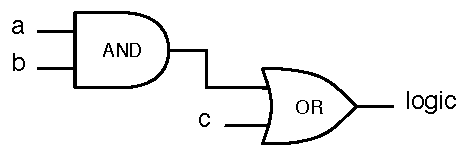
\includegraphics[scale=\scale]{figures/logic}
  \caption{Mạch logic cho biểu thức \code{(a \& b) | c}.
  Các đường nối dây có thể là bit đơn hoặc nhiều bit. Biểu thức trong Chisel, và bản vẽ mạch là như nhau.}
  \label{fig:logic}
\end{figure}


Hình~\ref{fig:logic} biểu diễn mạch điện của biểu thức mạch tổ hợp này.
Lưu ý rằng mạch điện này có thể dành cho vectơ các bit và không chỉ các dây đơn được kết hợp với các mạch AND và OR. 

Trong ví dụ này, chúng ta không định nghĩa kiểu dữ liệu, cũng không phải độ rộng của tín hiệu \code{logic}.
Cả hai đều được suy ra từ kiểu và độ rộng của biểu thức. 
Các phép toán logic chuẩn trong Chisel là:

\index{Phép toán logic}

\shortlist{code/bool_ops.txt}

\noindent Các phép toán số học sử dụng các toán tử chuẩn:

\index{Phép toán số học}

\shortlist{code/arith_ops.txt}

\noindent Độ rộng kết quả của phép toán là độ rộng tối đa của các toán tử cho phép cộng và phép trừ, 
tổng của hai độ rộng cho phép nhân và thường là độ rộng của tử số cho phép chia và phép toán chia lấy dư.\footnote{Chi tiết 
chính xác có trong \myref{https://github.com/freechipsproject/firrtl/blob/master/spec/spec.pdf}{Đặc tả FIRRTL}.}

Một tín hiệu ban đầu có thể được định nghĩa dưới dạng một số kiểu như \code{Wire}. Sau đó, chúng ta có thể gán
một giá trị với dây nối bởi toán tử cập nhật \code{:=}.

\shortlist{code/wire.txt}

Một bit đơn có thể được trích xuất như sau:
\shortlist{code/single_bit.txt}
\index{Bit!rút trích}

\noindent Một trường con có thể được trích xuất từ vị trí đầu đến cuối:
\shortlist{code/sub_field.txt}

\noindent Các trường bit được ghép nối bởi \code{Cat}.
\shortlist{code/concat.txt}
\index{Bit!ghép nối}

Bảng~\ref{tab:operators} trình bày danh sách đầy đủ của các toán tử
(xem thêm tại \myref{https://github.com/freechipsproject/chisel3/wiki/Builtin-Operators}{các toán tử nội tại}).
Mức độ ưu tiên của toán tử Chisel được xác định bởi thứ tự đánh giá của mạch, 
theo \myref{https://docs.scala-lang.org/tour/operators.html}{thứ tự ưu tiên của toán tử Scala}.
Nếu còn nghi ngờ, việc sử dụng dấu ngoặc đơn luôn là một phương pháp hay.\footnote{Độ ưu tiên toán tử trong Chisel
là một tác dụng phụ của việc chi tiết hóa phần cứng khi cấu trúc cây của các nút phần cứng 
được tạo ra bằng cách thực thi các toán tử Scala. Toán tử ưu tiên trong Scala tương tự nhưng không giống với Java/C. 
Verilog có cùng độ ưu tiên toán tử như C, nhưng VHDL lại có độ ưu tiên khác. Verilog có thứ tự ưu tiên cho các phép toán logic, 
nhưng trong VHDL các toán tử đó có cùng thứ tự ưu tiên và được đánh giá từ trái sang phải.}

Bảng~\ref{tab:functions} trình bày các hàm khác nhau được định nghĩa trên và cho các kiểu dữ liệu Chisel

\begin{table}
 \centering
 \label{tab:operators}
  \begin{tabular}{lll}
    \toprule
    Toán tử & Mô tả & Kiểu dữ liệu \\
    \midrule
    \code{* / \%} & nhân, chia, chia lấy dư & UInt, SInt \\
    \code{+ -} & cộng, trừ & UInt, SInt \\
    \code{=== =/=} & bằng, không bằng & UInt, SInt, returns Bool \\
    \code{> >= < <=} & so sánh & UInt, SInt, trả về Bool \\
    \code{<< >>} & dịch trái, dịch phải (mở rộng dấu cho SInt) & UInt, SInt \\
    \code{\~} & NOT & UInt, SInt, Bool \\
    \code{\& | \^} & AND, OR, XOR & UInt, SInt, Bool \\
    \code{!} & logic NOT & Bool \\
    \code{\&\& ||} & logic AND, OR & Bool \\
    \bottomrule 
  \end{tabular} 
  \caption{Các toán tử phần cứng được định nghĩa trên Chisel.}
\end{table}

\index{Toán tử}

\begin{table}
 \centering
 \label{tab:functions}
  \begin{tabular}{lll}
    \toprule
    Hàm & Mô tả & Kiểu dữ liệu \\
    \midrule
    \code{v.andR v.orR v.xorR} & AND, OR, XOR rút gọn & UInt, SInt, trả về Bool \\
    \code{v(n)} & trích xuất một bit đơn & UInt, SInt \\
    \code{v(end, start)} & trích xuất trường bit & UInt, SInt \\
    \code{Fill(n, v)} & sao chép chuỗi bit, n times & UInt, SInt \\
    \code{Cat(a, b, ...)} & ghép các trường bit & UInt, SInt \\
    \bottomrule 
  \end{tabular} 
  \caption{Các hàm phần cứng được định nghĩa trên Chisel, được gọi trên \code{v}.}
\end{table}

\index{Bit!rút gọn}
\index{Trường bit!rút trích}
\index{Trường bit!ghép nối}


\subsection{Mạch đa hợp}

\index{Mạch đa hợp}

\myref{https://en.wikipedia.org/wiki/Multiplexer}{Mạch đa hợp} là mạch chọn một trong nhiều ngõ vào đưa tới một ngõ ra (mạch đa hợp còn được gọi là mạch dồn kênh, mạch ghép kênh).
Ở dạng cơ bản nhất, mạch gồm có 2 ngõ vào. Hình~\ref{fig:mux} biểu diễn
mạch đa hợp 2:1, hay gọi là mux cho ngắn gọn. Tùy thuộc vào giá trị của
tín hiệu lựa chọn (tín hiệu \code{sel}), tín hiệu \code{y} sẽ biểu diễn tín hiệu \code{a} hoặc
tín hiệu \code{b}.

\begin{figure}
  \centering
  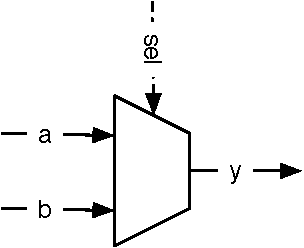
\includegraphics[scale=\scale]{figures/mux}
  \caption{Mạch đa hợp cơ bản 2:1.}
  \label{fig:mux}
\end{figure}

Mạch đa hợp có thể được hình thành từ các cổng logic.
Tuy nhiên, vì đa hợp là một phép toán chuẩn nên Chisel cung cấp mạch đa hợp,

\shortlist{code/mux.txt}

\noindent trong đó \code{a} được chọn khi \code{sel} là \code{true.B}, ngược lại \code{b}
sẽ được chọn. Kiểu dữ liệu \code{sel} là Chisel \code{Bool}; các ngõ vào \code{a} và \code{b}
có thể là bất kỳ kiểu cơ số Chisel hoặc kiểu tập hợp (bundles hoặc vectors) miễn là chúng cùng kiểu.

Với các phép toán logic và số học và đa hợp, mỗi một mạch đa hợp có thể được mô tả.
Tuy nhiên, Chisel cung cấp thêm các thành phần và điều khiển trừu tượng để mô tả một cách thanh thoát hơn về mạch tổ 
hợp, sẽ được mô tả trong chương sau.

Thành phần cơ bản thứ hai cẩn để mô tả mạch số là các thành phần trạng thái,
hay còn được gọi là thanh ghi, sẽ được mô tả ở phần tiếp theo.

\section{Các thanh ghi}

\index{Thanh ghi}
Chisel cung cấp thanh ghi, là tập hợp của các 
\myref{https://en.wikipedia.org/wiki/Flip-flop\_(electronics)\#D\_flip-flop}{flip-flop D}.
Thanh ghi được kết nối ngầm với xung clock toàn cục và được cập nhật trạng thái ở cạnh lên xung clock.
Khi giá trị khởi tạo được cung cấp lúc khai báo thanh ghi, nó sử dụng reset đồng bộ được nối với tín hiệu reset toàn cục.
Một thanh ghi ghi có thể là bất kỳ kiểu Chisel nào có thể được biểu diễn ở dạng tập hợp các bit.
Đoạn mã sau định nghĩa một thanh ghi 8-bit, được khởi tạo bằng 0 lúc reset:

\shortlist{code/register.txt}

\noindent Ngõ vào được nối với thanh ghi bởi toán tử cập nhật \code{:=} và
ngõ ra của thanh ghi có thể được sử dụng chỉ với tên trong biểu thức :

\shortlist{code/reg_con.txt}

\begin{figure}
  \centering
  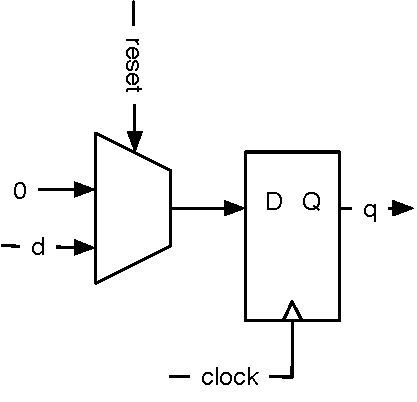
\includegraphics[scale=\scale]{figures/register-reset-0}
  \caption{Flip-flop D dựa trên thanh ghi với reset đồng bộ về 0.}
  \label{fig:register-reset-0}
\end{figure}

\noindent Một thanh ghi còn có thể được kết nối với chính ngõ vào của nó ở định nghĩa sau:

\shortlist{code/reg_next.txt}

Hình~\ref{fig:register-reset-0} biểu diễn mạch điện của định nghĩa thanh ghi với xung clock, tín hiệu reset đồng bộ với \code{0.U}, ngõ vào \code{d}, và ngõ ra \code{q}.
Các tín hiệu toàn cục \code{clock} và \code{reset} được kết nối ngầm với mỗi thanh ghi được định nghĩa.

\noindent Một thanh ghi còn có thể được kết nối với ngõ vào của nó và một hằng số như giá trị khởi tạo ở định nghĩa sau:

\shortlist{code/reg_both.txt}

\noindent Để phân biệt giữa các tín hiệu biểu diễn mạch logic tổ hợp và thanh ghi,
một thực tế phổ biến là đặt hậu tố các tên thanh ghi bởi \code{Reg}.
Một thực tế khác, đến từ Java và Scala, là sử dụng 
\myref{https://en.wikipedia.org/wiki/Camel_case}{camelCase} 
cho việc định danh bao gồm nhiều từ. Quy ước là bắt đầu các hàm 
và biến bằng chữ thường và bắt đầu các lớp (các kiểu) bằng chữ in hoa.

\subsection{Đếm}

\index{Đếm}

Đếm là một hoạt động cơ bản trong các hệ thống số. Nó có thể đếm các sự kiện. 
Tuy nhiên, đếm thường được sử dụng hơn để xác định một khoảng thời gian. 
Đếm chu kỳ xung clock và kích hoạt một hoạt động khi khoảng thời gian đã hết.

Một cách tiếp cận đơn giản là đếm lên một giá trị. Tuy nhiên, trong khoa học máy tính,
và thiết kế mạch số, việc đếm bắt đầu từ 0. Do đó, nếu chúng ta muốn đếm đến 10, 
thì chúng ta đếm từ 0 đến 9. Đoạn mã sau đây cho thấy một mạch đếm như vậy: đếm đến 9 và quay về 0 khi đạt đến 9.

\shortlist{code/counter.txt}

\section{Cấu trúc với Bundle và Vec}

\index{Cấu trúc}
\index{Mảng}
\index{Tập hợp}
\index{Véc-tơ}
\index{Bundle}

Chisel cung cấp hai cấu trúc để nhóm các tín hiệu liên quan với nhau: (1) \code{Bundle} để nhóm
các tín hiệu có kiểu khác nhau và (2) \code{Vec} để biểu diễn tập hợp các tín hiệu cùng kiểu có thể truy xuất được.
Các \code{Bundle} và \code{Vec} có thể được lồng vào nhau tùy ý.

Một bundle trong Chisel nhóm nhiều tín hiệu. Toàn thể bundle có thể được tham chiếu
toàn bộ chung, hoặc các trường riêng rẽ có thể được truy cập bởi tên của chúng.
Chúng ta có thể định nghĩa một bundle (tập hợp của các tín hiệu) bằng cách định nghĩa một lớp 
mở rộng \code{Bundle} và liệt kê các trường như \code{val}s trong khối cấu trúc.

\shortlist{code/bundle.txt}

\noindent Để sử dụng bundle, chúng ta tạo nó bởi từ khóa \code{new} và bọc (wrap) nó thành một kiểu \code{Wire}.
Các trường được truy cập bởi dấu chấm:

\shortlist{code/bundle_use.txt}

Ký hiệu dấu chấm phổ biến trong các ngôn ngữ hướng đối tượng, với \code{x.y} có nghĩa
\code{x} là một tham chiếu đến đối tượng và \code{y} là trường của đối tượng đó.
Vì Chisel là hướng đối tượng, nên chúng ta sử dụng ký hiệu dấu chấm để truy cập các trường trong bundle.
Bundle tương tự với \code{struct} trong C, \code{record} trong VHDL, hoặc
\code{struct} trong SystemVerilog.
Bundle cũng có thể được tham chiếu một cách tổng thể:

\shortlist{code/bundle_ref.txt}

\code{Vec} trong Chisel biểu diễn tập hợp các tín hiệu có cùng kiểu (véc-tơ).
Mỗi thành phần có thể được truy cập bởi một chỉ số. \code{Vec} trong Chisel tương tự với 
cấu trúc mảng dữ liệu trong các ngôn ngữ lập trình khác.\footnote{Tên \codefoot{Array}
đã được sử dụng trong Scala.}
\code{Vec} được tạo bằng cách gọi cấu trúc với hai tham số: số phần tử và kiểu phần tử. 
\code{Vec} tổ hợp cần được bọc thành kiểu \code{Wire.}

\shortlist{code/vec.txt}

\noindent Các thành phần riêng rẽ được truy cập bởi \code{(index)}.

\shortlist{code/vec_access.txt}

Một véc-tơ được bọc thành \code{Wire} là mạch đa hợp.
Chúng ta có thể bọc một véc-tơ thành một thanh ghi để định nghĩa một mảng các thanh ghi.
Ví dụ sau định nghĩa một tập thanh ghi cho một bộ xử lý; 32 thanh ghi, mỗi thanh ghi 32-bit
như trong bộ xử lý 32-bit \myref{https://en.wikipedia.org/wiki/Reduced_instruction_set_computer}{RISC}, giống 
phiên bản 32-bit của \myref{https://en.wikipedia.org/wiki/RISC-V}{RISC-V}.

\shortlist{code/reg_file.txt}

\noindent Một phần tử của tập thanh ghi đó được truy cập bằng một chỉ số và được sử dụng như một thanh ghi bình thường.

\shortlist{code/reg_file_access.txt}

Chúng ta có thể tự do trộn bundle và véc-tơ với nhau. Khi tạo một véc-tơ với kiểu 
bundle, chúng ta có thể chuyển một nguyên mẫu của các trường véc-tơ. Sử dụng 
\code{Channel}, đã được định nghĩa ở trên, chúng ta có thể tạo véc-tơ của các kênh với:

\shortlist{code/vec_bundle.txt}

\noindent Một bundle cũng có thể chứa một véc-tơ:

\shortlist{code/bundle_vec.txt}

Khi chúng ta muốn một thanh ghi của kiểu bundle cần một giá trị reset,
đầu tiên cần tạo \code{Wire} của bundle đó, đặt giá trị các trường riêng lẻ nếu cần, 
và sau đó chuyển bundle này thành \code{RegInit}:

\shortlist{code/bundle_reg_init.txt}

Với sự kết hợp của \code{Bundle}s và \code{Vec}s chúng ta có thể định nghĩa các cấu trúc dữ liệu riêng của mình,
đó là những sự trừu tượng mạnh mẽ.

\section{Chisel tạo phần cứng}

Sau khi tham khảo một số mã code ban đầu của Chisel, chúng ta thấy nó tương tự như các
ngôn ngữ lập trình cổ điển như Java hay C. Tuy nhiên, Chisel (hoặc bất kỳ các ngôn ngữ
mô tả phần cứng khác) định nghĩa các thành phần phần cứng. Trong một chương trình
phần mềm, một dòng code chỉ được thi hành sau khi dòng khác được thi hành, trong khi đó 
trong phần cứng tất cả các dòng code đều được \emph{thực thi song song}.

Điều quan trọng cần nhớ là mã Chisel tạo ra phần cứng. 
Hãy thử tưởng tượng, hoặc vẽ trên một tờ giấy, các khối riêng lẻ được 
tạo ra bởi mô tả mạch điện Chisel của các bạn. Mỗi lần tạo thành phần sẽ thêm phần cứng; 
mỗi câu lệnh gán tạo ra các cổng và/hoặc các flip-flop.

Về mặt kỹ thuật, khi Chisel thực thi mã của các bạn, nó sẽ chạy như một chương trình Scala,
và bằng cách thực thi các câu lệnh Chisel, nó \emph{thu thập} các thành phần phần cứng
và kết nối các nút đó lại với nhau. Mạng lưới các nút phần cứng này là phần cứng, 
có thể thành mã Verilog để tổng hợp ASIC hoặc FPGA hoặc có thể được kiểm tra bằng trình kiểm tra Chisel. 
Mạng các nút phần cứng được thực thi hoàn toàn song song.

Đối với một kỹ sư phần mềm, hãy tưởng tượng sự song song to lớn này có thể 
tạo ra trong phần cứng mà không cần phân vùng ứng dụng thành các luồng
và nhận khóa chính xác cho giao tiếp.

\section{Bài tập}

Trong phần giới thiệu, các bạn đã thực hiện đèn LED nhấp nháy trên bo mạch FPGA
(ở thư mục \myref{https://github.com/schoeberl/chisel-examples}{chisel-examples}), đó là một ví dụ \emph{Hello World} 
hợp lý về phần cứng. Nó chỉ sử dụng các trạng thái bên trong, một đèn LED ngõ ra, và không có ngõ vào.
Chép dự án này vào một thư mục mới và mở rộng nó bằng cách thêm một số ngõ vào ở \code{io} \code{Bundle}
với \code{val sw = Input(UInt(2.W))}.

\shortlist{code/basic_exercise.txt}

\noindent Với những công tắc này, các bạn còn cần gán tên chân cho bo mạch FPGA.
Các bạn có thể tìm ví dụ gán chân trên tập tin dự án Quartus qua dự án ALU
(Ví dụ: trên bo mạch \myref{https://github.com/schoeberl/chisel-examples/blob/master/quartus/altde2-115/alu.qsf}{FPGA DE2-115}).

Khi các bạn đã định nghĩa các ngõ vào đó và gán chân, hãy bắt đầu với một bài kiểm tra đơn giản: 
loại bỏ tất cả logic nhấp nháy khỏi thiết kế và kết nối một công tắc với ngõ ra LED; 
biên dịch và cấu hình thiết bị FPGA. Các bạn có thể gạt công tắc đèn LED bật hay tắt không? 
Nếu có, bạn đã có các ngõ vào có sẵn. Nếu không, bạn cần gỡ lỗi cấu hình FPGA của mình. 
Việc gán chân cũng có thể được thực hiện với phiên bản GUI của công cụ.

Bây giờ sử dụng hai công tắc và thực hiện một trong những hàm mạch tổ hợp cơ bản, 
ví dụ: hai công tắc cho hai ngõ vào AND và hiển thị kết quả trên đèn LED. Thay đổi chức năng. 
Bước tiếp theo liên quan đến ba công tắc ngõ vào để thực hiện mạch đa hợp: một công tắc hoạt động 
như tín hiệu chọn và hai công tắc còn lại là hai ngõ vào cho mạch đa hợp 2:1.

Bây giờ, các bạn đã có thể thực hiện các hàm của mạch tổ hợp đơn giản và kiểm tra chúng
trong phần cứng thực sự trên FPGA. Bước tiếp theo, chúng ta sẽ xem làm thế nào quá trình xây dựng hoạt động
để tạo cấu hình cho FPGA. Hơn nữa, chúng ta cũng sẽ khám phá một khung sườn kiểm tra đơn giản từ Chisel,
cho phép các bạn kiểm tra mạch điện mà không cần cấu hình FPGA và chuyển đổi công tắc.

\chapter{Xây dựng quy trình và kiểm tra}

Để bắt đầu với các đoạn mã Chisel thú vị hơn, trước tiên chúng ta cần học cách biên dịch
các chương trình Chisel, cách tạo mã Verilog để thực thi trong FPGA và cách viết 
các bài kiểm tra để gỡ lỗi và kiểm tra rằng các mạch điện của chúng ta có hoạt động đúng hay không.

Chisel được viết bằng Scala, vì vậy bất kỳ quá trình xây dựng nào hỗ trợ Scala đều có thể thực hiện
được với dự án Chisel. Một công cụ xây dựng phổ biến cho Scala là \myref{https://www.scala-sbt.org/}{sbt},
viết tắt của công cụ xây dựng tương tác Scala (Scala interactive Build Tool).
Bên cạnh việc thúc đẩy quá trình xây dựng và kiểm tra, \code{sbt} cũng sẽ tải xuống phiên bản đúng của thư viện Scala và Chisel.

\section{Xây dựng dự án với sbt}

\index{sbt}

Thư viện Scala đại diện cho Chisel và trình kiểm tra Chisel được tự động tải xuống 
trong quá trình xây dựng từ kho lưu trữ Maven. Các thư viện được 
tham chiếu bởi \code{build.sbt}. Có thể cấu hình \code{build.sbt} bằng \code{last.release} để luôn luôn sử dụng phiên bản Chisel cập nhật nhất. Tuy nhiên, điều này có nghĩa là trên mỗi lần build (xây dựng), phiên bản được tra cứu từ kho lưu trữ Maven. Việc tra cứu này cần có kết nối Internet để việc build thành công. Tốt hơn hãy sử dụng phiên bản Chisel chuyên dụng và tất cả các thư viện Scala khác trong \code{build.sbt} của bạn. Có lẽ đôi khi cũng tốt khi có thể viết mã code phần cứng và kiểm tra nó mà không cần kết nối Internet.
Ví dụ, thật tuyệt khi thiết kế phần cứng ở trên máy bay.

\subsection{Tổ chức nguồn}

\index{Tổ chức nguồn}

\code{sbt} kế thừa các quy ước nguồn từ công cụ build tự động \myref{https://maven.apache.org/}{Maven.}
Maven còn tổ chức các kho thư viện Java mã nguồn mở.\footnote{Đó cũng là nơi các bạn đã tải xuống thư viện Chisel 
trong lần build đầu tiên của mình:
\url{https://mvnrepository.com/artifact/edu.berkeley.cs/chisel3}.}

\begin{figure}
\dirtree{%
.1 project.
.2 src.
.3 main.
.4 scala.
.5 package.
.6 sub-package.
.3 test.
.4 scala.
.5 package.
.2 target.
.2 generated.
}
\caption{Cấu trúc cây nguồn của một dự án Chisel (sử dụng \code{sbt})}
\label{fig:folders}
\end{figure}

Hình~\ref{fig:folders} biểu diễn tổ chức của cấu trúc cây nguồn (source tree) của một dự án Chisel tiêu biểu.
Thư mục gốc của dự án là thư mục nhà (thư mục home) của dự án, chứa tập tin \code{build.sbt}.
Nó còn bao gồm tập tin \code{Makefile} cho quy trình build, tập tin README, và một tập tin LICENSE.
Thư mục \code{src} chứa tất cả mã nguồn. Từ đó, nó được tách giữa thư mục \code{main},
chứa nguồn phần cứng và thư mục \code{test} chứa trình kiểm tra.
Chisel thừa hưởng từ Scala, vốn kế thừa từ Java cấu trúc nguồn
trong \myref{https://en.wikipedia.org/wiki/Java_package}{các gói}.
Các gói tổ chức mã Chisel của bạn trong các không gian tên. Các gói còn có thể chứa các gói con.
Thư mục \code{target} chứa các tập tin lớp và các tập tin khác được tạo ra.
Tôi khuyên là cũng nên sử dụng một thư mục chứa các tập tin Verilog được tạo ra, thường gọi là thư mục \code{generated}.

Để sử dụng các phương diện trong không gian tên của Chisel, các bạn cần khai báo lớp/mô-đun
được định nghĩa trong gói, trong ví dụ này \code{mypack}:

\shortlist{code/mypack.txt}

\noindent Lưu ý rằng trong ví dụ này, chúng ta thấy việc nhập của gói \code{chisel3} 
để sử dụng các lớp Chisel.

Để sử dụng mô-đun \code{Abc} trong một ngữ cảnh khác (gói không gian tên),
các thành phần của gói \code{mypack} cần phải được nhập vào. Dấu gạch dưới
(\_) đóng vai trò là ký tự đại diện, nghĩa là tất cả các lớp của \code{mypack} được nhập.

\shortlist{code/usemypack.txt}

\noindent Cũng có khả năng là không nhập tất cả các kiểu từ \code{mypack},
nhưng sử sụng tên đủ điều kiện \code{mypack.Abc} để đưa đến mô-đun
\code{Abc} trong gói \code{mypack}.

\shortlist{code/usemypack2.txt}

\noindent Cũng có thể nhập vào chỉ một lớp duy nhất và tạo một thực thể của nó:

\shortlist{code/usemypack3.txt}

\subsection{Chạy chương trình sbt}

Một dự án Chisel có thể được biên dịch và thi hành với một lệnh \code{sbt} đơn giản:

\begin{verbatim}
$ sbt run
\end{verbatim}

Lệnh này sẽ biên dịch tất cả các mã Chisel của bạn từ cấu trúc cây nguồn và tìm kiếm các lớp chứa
\code{object} bao gồm phương pháp \code{main}, hoặc đơn giản hơn là mở rộng \code{App}. 
Nếu có nhiều hơn một đối tượng, thì tất cả các đối tượng được liệt kê và và một đối tượng có thể được chọn.
Các bạn còn có thể xác định trực tiếp đối tượng sẽ được thi hành như là một tham số đối với \code{sbt}:

\begin{verbatim}
$ sbt "runMain mypacket.MyObject"
\end{verbatim}

Theo mặc định, \code{sbt} chỉ tìm kiếm phần \code{main} của cấu trúc cây nguồn, chứ không tìm kiếm phần
\code{test}.\footnote{Đây là dạng quy ước của Java/Scala rằng thư mục test chứa 
các bài kiểm tra đơn vị chứ không phải các đối tượng với \codefoot{main}.} Tuy nhiên, các trình kiểm tra Chisel, 
như đã được mô tả ở đây, chứa \code{main}, nhưng sẽ được đặt trong phần \code{test} của source tree.
Để thực thi \code{main} trong cấu trúc cây của trình kiểm tra, sử dụng lệnh \code{sbt} sau:

\begin{verbatim}
$ sbt "test:runMain mypacket.MyTester"
\end{verbatim}

Bây giờ chúng ta biết được cấu trúc cơ bản của một dự án Chisel và cách để biên dịch và chạy nó
với \code{sbt}, chúng ta có thể tiếp tục với một khung sườn kiểm tra đơn giản.

\subsection{Quy trình công cụ}

\begin{figure}
  \centering
  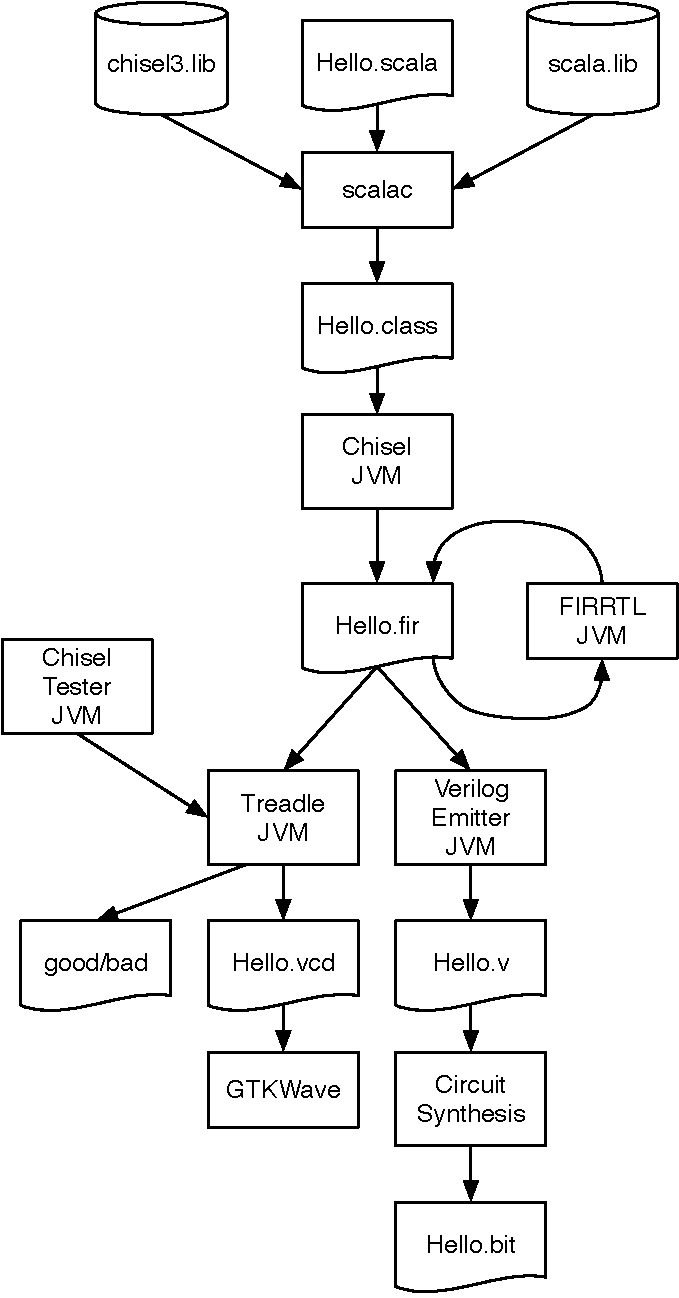
\includegraphics[scale=\scale]{figures/flow}
  \caption{Quy trình công cụ của hệ sinh thái Chisel.}
  \label{fig:flow}
\end{figure}

Hình~\ref{fig:flow} trình bày quy trình công cụ của Chisel. Mạch số được mô tả trong một lớp Chisel
được trình bày trong \code{Hello.scala}. Trình biên dịch Scala sẽ biên dịch lớp này, cùng với các thư viện Chisel và Scala,
và tạo ra lớp Java \code{Hello.class} có thể được thực thi bởi 
\myref{https://en.wikipedia.org/wiki/Java_virtual_machine}{Máy ảo Java (JVM)} chuẩn.

Việc thực thi lớp này với trình điều khiển Chisel tạo ra cái gọi là dạng biểu diễn trung gian linh hoạt cho RTL (FIRRTL), 
một dạng biểu diễn trung gian của các mạch số. Trong ví dụ, tập tin biểu diễn trung gian là \code{Hello.fir}. 
Trình biên dịch FIRRTL thực hiện các phép biến đổi trên mạch điện.

Treadle là một trình thông dịch FIRRTL để mô phỏng mạch điện. Cùng với trình kiểm tra Chisel, 
nó có thể được sử dụng để gỡ lỗi và kiểm tra các mạch điện của Chisel. Với các giá trị ngõ vào, chúng có thể đưa ra các
kết quả kiểm tra. Treadle cũng có thể tạo ra các tập tin dạng sóng (\code{Hello.vcd}), chúng có thể được xem bằng 
chương trình xem dạng sóng (Ví dụ: các chương trình xem miễn phí như GTKWave hoặc Modelsim).

Một phép biến đổi FIRRTL, hay bộ phát Verilog, sẽ tạo mã Verilog để tổng hợp mạch (\code{Hello.v}). 
Một công cụ tổng hợp mạch (Ví dụ: Intel Quartus, Xilinx Vivado hoặc một công cụ ASIC) sẽ tổng hợp mạch điện.
Trong quy trình thiết kế FPGA, công cụ tạo tập tin bitstream FPGA được sử dụng để cấu hình cho FPGA, ví dụ: \code{Hello.bit}.

\section{Kiểm tra với Chisel}

\index{Kiểm tra}

Các kiểm tra cho các thiết kế phần cứng thường được gọi là \myref{https://www.xilinx.com/support/documentation/sw_manuals/xilinx10/isehelp/ise_c_simulation_test_bench.htm}{testbench}.
Testbench khởi tạo các thiết kế cần được kiểm tra (Design under Test - DUT), điều khiển các ngõ vào, quan sát các ngõ ra,
và so sánh chúng với các giá trị mong đợi.

\subsection{PeekPokeTester}

Chisel cung cấp các testbench dưới dạng \code{PeekPokeTester}.
Một điểm mạnh của Chisel là nó có thể sử dụng toàn bộ sức mạnh của Scala để viết
các testbench đó. Ví dụ, một người có thể viết mã với chức năng mong đợi của phần cứng 
trong một chương trình mô phỏng phần mềm và so sánh kết quả mô phỏng của phần cứng với chương trình mô phỏng
phần mềm. Phương pháp này rất hiệu quả khi kiểm tra việc thực hiện một bộ xử lý~\cite{lipsi:arcs2018}.

Để sử dụng \code{PeekPokeTester}, các gói sau cần được nhập vào (import):

\shortlist{code/test_import.txt}

\noindent Việc kiểm tra một mạch điện có (ít nhất) ba thành phần: (1) thiết bị được kiểm tra (thường 
được gọi là DUT), (2) giá trị logic để kiểm tra, còn được gọi là testbench và (3) các đối tượng của trình kiểm tra 
có chứa \code{main} để bắt đầu việc kiểm tra.

Đoạn mã sau đây trình bày thiết kế đơn giản của chúng ta đang được thử nghiệm. Nó chứa hai 
cổng ngõ vào và một cổng ngõ ra, tất cả đều có độ rộng 2-bit. Mạch điện thực hiện phép toán AND bit-wise 
để trả về giá trị ngõ ra:

\shortlist{code/test_dut.txt}

\noindent Testbench cho DUT này mở rộng \code{PeekPokeTester} và có DUT như là tham số cho hàm tạo:

\shortlist{code/test_bench_simple.txt}

\noindent \code{PeekPokeTester} có thể đặt giá trị ngõ vào với \code{poke()} và
đọc ngược các giá trị ngõ ra với \code{peek()}. Trình kiểm tra tăng quá trình mô phỏng thêm
một bước (= một chu kỳ xung clock) với \code{step(1)}.
Chúng ta có thể in các giá trị ngõ ra bởi \code{println()}.

Kiểm tra được tạo và chạy với chương trình kiểm tra chính sau:

\shortlist{code/test_main_simple.txt}

\noindent Khi các bạn chạy kiểm tra, các bạn sẽ thấy kết quả được in ra ở terminal (bên cạnh các thông tin khác):

\begin{verbatim}
[info] [0.004] SEED 1544207645120
[info] [0.008] Result is: 0
[info] [0.009] Result is: 2
test DeviceUnderTest Success: 0 tests passed in 7 cycles
taking 0.021820 seconds
[info] [0.010] RAN 2 CYCLES PASSED
\end{verbatim}

\noindent Chúng ta thấy rằng 0 AND 1 cho kết quả là 0; 3 AND 2 cho kết quả là 2.
Bên cạnh việc đánh giá các kết quả xuất ra theo cách thủ công, vốn là một điểm khởi đầu tuyệt vời, chúng ta 
cũng có thể tbiểu diễn kết quả mong đợi của mình trong chính testbench với \code{expect()}, có cổng ngõ ra 
và giá trị mong đợi dưới dạng các tham số. Ví dụ sau trình bày việc kiểm tra với \code{expect()}:

\shortlist{code/test_bench.txt}

\noindent Thực thi việc kiểm tra này không xuất ra bất kỳ giá trị nào từ phần cứng,
nhưng tất cả bài kiểm tra đều được PASSED khi tất cả giá trị mong đợi đều đúng.

\begin{verbatim}
[info] [0.001] SEED 1544208437832
test DeviceUnderTest Success: 2 tests passed in 7 cycles
taking 0.018000 seconds
[info] [0.009] RAN 2 CYCLES PASSED
\end{verbatim}

\noindent Kiểm tra không thành công, khi DUT hoặc testbench có lỗi, sẽ tạo ra một thông báo 
lỗi mô tả sự sai biệt giữa giá trị kỳ vọng và giá trị thực tế. Trong phần sau, chúng ta 
thay đổi testbench để kỳ vọng kết quả là 4, đó là một lỗi:

\begin{verbatim}
[info] [0.002] SEED 1544208642263
[info] [0.011] EXPECT AT 2   io_out got 0 expected 4 FAIL
test DeviceUnderTest Success: 1 tests passed in 7 cycles
taking 0.022101 seconds
[info] [0.012] RAN 2 CYCLES FAILED FIRST AT CYCLE 2
\end{verbatim}

Trong phần này, chúng ta mô tả phương tiện kiểm tra cơ bản với Chisel cho các kiểm tra đơn giản.
Tuy nhiên, trong Chisel, toàn bộ sức mạnh của Scala có sẵn để viết các trình kiểm tra. 
\todo{Có một liên kết đến phần này chưa được viết: Chúng tôi sẽ trình bày sau.}

\subsection{Sử dụng ScalaTest}

\index{ScalaTest}

\myref{http://www.scalatest.org/}{ScalaTest} là một công cụ kiểm tra dành cho Scala (và Java),
mà chúng ta có thể sử dụng để chạy các chương trình kiểm tra Chisel.
Để sử dụng nó, bao gồm thư viện trong \code{build.sbt} của các bạn với dòng lệnh sau:

\begin{chisel}
libraryDependencies += "org.scalatest" %% "scalatest" % "3.0.5" % "test"
\end{chisel}

\noindent Các bài kiểm tra thường được tìm thấy trong \code{src/test/scala} và có thể được chạy bởi lệnh:

\begin{verbatim}
$ sbt test
\end{verbatim}

\noindent Một kiểm tra tối thiểu (kiểm tra Hello World) để kiểm tra cộng số nguyên trong Scala:

\shortlist{code/scalatest_hello_world.txt}

\noindent Mặc dù kiểm tra trên Chisel nặng nề hơn kiểm tra đơn vị của các chương trình Scala, 
chúng ta có thể kết hợp kiểm tra Chisel thành một lớp ScalaTest. Đối với \code{Tester} được hiển thị trước đây là:

\shortlist{code/scalatest_simple.txt}

Lợi ích chính của bài tập này là có thể chạy tất cả các trình kiểm tra với một lệnh \code{sbt test} 
đơn giản (thay vì chạy \code{main}). Các bạn có thể chạy chỉ một trình kiểm tra duy nhất với \code{sbt} như sau:

\begin{verbatim}
$ sbt "testOnly SimpleSpec"
\end{verbatim}

\subsection{Dạng sóng}

Các chương trình kiểm tra, như đã đề cập ở trên, làm việc tốt với các thiết kế nhỏ và
\myref{https://en.wikipedia.org/wiki/Unit_testing}{kiểm tra đơn vị}, vì nó phổ biến trong phát 
triển phần mềm. Một tập hợp các bài kiểm tra đơn vị cũng có thể dùng cho
\myref{https://en.wikipedia.org/wiki/Regression_testing}{kiểm tra hồi quy}.

Tuy nhiên, để gỡ lỗi các thiết kế phức tạp hơn, người ta muốn xét nhiều tín hiệu cùng lúc. 
Một cách tiếp cận cổ điển để gỡ lỗi các thiết kế mạch số là hiển thị 
các tín hiệu dưới dạng sóng. Ở dạng sóng, các tín hiệu được hiển thị theo thời gian.

Các chương trình kiểm tra có thể tạo ra một dạng sóng bao gồm tất cả các thanh ghi và tất cả các tín hiệu vào ra IO. 
Trong các ví dụ sau, chúng ta hiển thị chương trình kiểm tra dạng sóng cho \code{DeviceUnderTest} 
từ ví dụ trước (hàm AND 2-bit). Với ví dụ sau, chúng ta nhập các lớp sau:

\shortlist{code/test_import_wave.txt}

\noindent Chúng ta bắt đầu với một trình kiểm tra đơn giản, lấy giá trị của các ngõ vào và tăng xung clock 
bằng lệnh \code{step}. Chúng ta không đọc bất kỳ ngõ ra nào hoặc so sánh nó với \code{kết quả mong đợi}.

\shortlist{code/test_bench_wave.txt}

\noindent Thay vì chúng ta gọi \code{Driver.execute} với các tham số để tạo các tập tin dạng sóng (tập tin .vcd).

\shortlist{code/scalatest_wave.txt}

Các bạn có thể xem dạng sóng với các công cụ miễn phí như GTKWave hoặc ModelSim.
Chạy GTKWave và chọn \emph{File -- Open New Window} và chuyển đến thư mục mà trình kiểm tra
Chisel đặt tập tin \code{.vcd}. Theo mặc định, các tập tin được tạo ra ở trong 
thư mục \code{test\_run\_dir} sau đó tên của chương trình kiểm tra được đánh thêm số ở phía sau.
Ở trong thư mục này, các bạn có thể thấy tập tin \code{DeviceUnderTest.vcd}.
Các bạn có thể lựa chọn các tín hiệu từ bên trái và kéo chúng vào cửa sổ chính.
Nếu các bạn muốn lưu cấu hình của các tín hiệu, các bạn thực hiện bằng cách vào 
\emph{File -- Write Save File} và sau đó có thể mở chúng lại bằng cách vào \emph{File -- Read Save File}.

Liệt kê rõ ràng tất cả các giá trị ngõ vào không chia tỷ lệ. Do đó, chúng ta sử dụng một số 
mã Scala để điều khiển DUT. Trình kiểm tra sau liệt kê tất cả các giá trị có thể có cho 
2 tín hiệu ngõ vào 2-bit.

\shortlist{code/test_bench_wave_cnt.txt}

\noindent Chúng ta thêm đặc tả ScalaTest cho trình kiểm tra mới này

\shortlist{code/scalatest_wave_cnt.txt}

\noindent và thực thi với lệnh

\begin{verbatim}
sbt "testOnly WaveformCounterSpec"
\end{verbatim}

\subsection{Gỡ lỗi với printf}

Một hình thức gỡ lỗi khác là cái gọi là ``gỡ lỗi printf''. Hình thức này đơn giản chỉ là đặt 
các câu lệnh \code{printf} trong C để in ra giá trị các biến chúng ta quan tâm trong quá trình 
thực thi chương trình. Gỡ lỗi printf này cũng có sẵn trong quá trình kiểm tra các mạch điện Chisel. 
Việc in các giá trị xảy ra ở cạnh lên của xung clock. Câu lệnh \code{printf} có thể được chèn vào 
bất kỳ đâu trong định nghĩa mô-đun, như được trình bày trong phiên bản gỡ lỗi printf của DUT.

\shortlist{code/test_dut_printf.txt}

\noindent Khi kiểm tra mô-đun này với trình kiểm tra dựa trên mạch đếm, lặp lại trên tất cả các giá 
trị có thể, chúng ta nhận được kết quả ngõ ra sau, xác minh rằng hàm AND là đúng:

\begin{verbatim}
Circuit state created
[info] [0.001] SEED 1579707298694
dut: 0 0 0
dut: 0 1 0
dut: 0 2 0
dut: 0 3 0
dut: 1 0 0
dut: 1 1 1
dut: 1 2 0
dut: 1 3 1
dut: 2 0 0
dut: 2 1 0
dut: 2 2 2
dut: 2 3 2
dut: 3 0 0
dut: 3 1 1
dut: 3 2 2
dut: 3 3 3
test DeviceUnderTestPrintf Success: 0 tests passed in 21 cycles
  taking 0.036380 seconds
[info] [0.024] RAN 16 CYCLES PASSED
\end{verbatim}

Lệnh printf Chisel hỗ trợ 
\myref{https://github.com/freechipsproject/chisel3/wiki/Printing-in-Chisel}{định dạng như trong C và Scala}.


\section{Bài tập}

Với bài tập phần này, chúng ta sẽ xem lại bài đèn LED nhấp nháy từ
\myref{https://github.com/schoeberl/chisel-examples}{chisel-examples}
và phám khá kiểm tra Chisel. \todo{Cũng sử dụng ví dụ ALU.}

\subsection{Dự án tối thiểu}

Đầu tiên, chúng ta hãy cùng tìm hiểu dự án Chisel tối thiểu là gì. Khám phá các tập tin trong ví dụ
\myref{https://github.com/schoeberl/chisel-examples/tree/master/hello-world}{Hello World}.
\code{Hello.scala} là tập tin nguồn phần cứng duy nhất.
Nó chứa mô tả phần cứng của đèn LED nhấp nháy (\code{class Hello})
và \code{App} tạo mã Verilog.

Mỗi tập tin bắt đầu với việc nhập Chisel và các gói liên quan:

\shortlist{code/import.txt}

\noindent Sau đó theo mô tả phần cứng, như đã trình bày trong Listing~\ref{lst:chisel:hello}.
Để tạo mô tả Verilog, chúng ta cần một ứng dụng. Một đối tượng Scala \code{extends App}
là một ứng dụng ngầm tạo hàm chính nơi ứng dụng đó khởi động.
Hành động duy nhất của ứng dụng này là tạo ra một đối tượng \code{HelloWorld} mới và chuyển nó vào 
trình điều khiển Chisel \code{execute} hàm. Đối số đầu tiên là một mảng Strings,
nơi các tùy chọn cho việc build có thể được đặt (ví dụ, thư mục ngõ ra). Đoạn mã sau sẽ tạo ra
tập tin Verilog \code{Hello.v}.

\shortlist{code/generate.txt}

\noindent Chạy quá trình tạo ví dụ theo cách thủ công với lệnh

\begin{chisel}
$ sbt "runMain Hello"
\end{chisel}

và khám phá tập tin \code{Hello.v} được tạo ra với một trình soạn thảo. Mã Verilog được tạo ra có thể không đọc được 
nhưng chúng ta có thể tìm hiểu một số chi tiết. Tập tin bắt đầu với mô-đun \code{Hello},
có cùng tên với mô-đun Chisel của chúng ta. Chúng ta có thể xác định cổng LED là ngõ ra
\code{output io\_led}. Tên các chân là tên Chisel với \code{io\_} ở trước.
Bên cạnh chân LED, mô-đun còn chứa các tín hiệu ngõ vào là \code{clock} và \code{reset}.
Hai tín hiệu này được thêm vào tự động bởi Chisel.

Hơn nữa, chúng ta có thể xác định định nghĩa của hai thanh ghi \code{cntReg} và \code{blkReg}.
Chúng ta còn có thể thấy reset và cập nhật các thanh ghi này ở cuối định nghĩa của mô-đun.
Lưu ý rằng Chisel tạo reset đồng bộ.

Để \code{sbt} có thể gọi trình biên dịch Scala và thư viện Chisel đúng,
chúng ta cần lệnh \code{build.sbt} sau:

\begin{chisel}
scalaVersion := "2.12.12"

scalacOptions := Seq("-deprecation", "-Xsource:2.11")

resolvers ++= Seq(
  Resolver.sonatypeRepo("snapshots"),
  Resolver.sonatypeRepo("releases")
)

libraryDependencies += "edu.berkeley.cs" %% "chisel-iotesters" % "1.5.1"
libraryDependencies += "edu.berkeley.cs" %% "chiseltest" % "0.3.1"
// Chisel 3.4.1 is loaded as a dependency on the testers
\end{chisel}

\noindent Lưu ý rằng trong ví dụ này, chúng ta có số phiên bản Chisel cụ thể để tránh kiểm tra 
phiên bản mới ở mỗi lần chạy (sẽ không thực hiện được nếu không có kết nối với Internet, 
ví dụ: khi thiết kế phần cứng trên máy bay).
Thay đổi cấu hình \code{build.sbt} để sử dụng phiên bản Chisel mới nhất bằng cách thay đổi 
lệnh trong phần thư viện như sau
\begin{chisel}
libraryDependencies += "edu.berkeley.cs" %% "chisel3" % "latest.release"
\end{chisel}

\noindent và chạy lại build với lệnh \code{sbt}. Xem có phiên bản Chisel mới hơn không và 
nó có được tải xuống tự động không? 

Để thuận tiện, thư mục dự án cũng chứa một tập tin \code{Makefile}.
Trong tập tin này chỉ có lệnh \code{sbt}, vì vậy chúng ta không cần nhớ nó 
và có thể tạo mã Verilog với lệnh:

\begin{chisel}
make
\end{chisel}

%The project also contains a
%\myref{https://github.com/schoeberl/chisel-examples/blob/master/hello-world/verilog/hello_top.v}{Verilog top level},
%which wires the reset signal to 0.
%This works for our example in an FPGA, as registers usually power up 0.
Bên cạnh tập tin \code{README}, thư mục dự án cũng chứa các tập tin dự án cho bo mạch FPGA khác nhau.
Ví dụ, trong
\myref{https://github.com/schoeberl/chisel-examples/tree/master/hello-world/quartus/altde2-115}{quartus/altde2-115} 
các bạn có thể thấy hai tập tin dự án để định nghĩa một dự án Quartus cho bo mạch DE2-115. 
Các định nghĩa chính (tập tin nguồn, thiết bị, gán chân) có thể được tìm thấy trong tập tin văn bản
\myref{https://github.com/schoeberl/chisel-examples/blob/master/hello-world/quartus/altde2-115/hello.qsf}{hello.qsf}.
Khám phá tập tin và xem chân nào được nối với tín hiệu nào.
Nếu các bạn cần chuyển dự án sang một bo mạch khác, thì ở đó các thay đổi được cập nhật.
Nếu bạn có chương trình Quartus đã cài đặt, mở dự án đó, biên dịch với nút \emph{Play} xanh lá,
và sau đó cấu hình cho FPGA.

Lưu ý rằng \emph{Hello World} là dự án Chisel tối thiểu.
Các dự án thực tế hơn có các tập tin nguồn được tổ chức thành các gói và chứa các trình kiểm tra.
Bài tập tiếp theo sẽ khám phá một dự án như vậy.

\subsection{Bài tập kiểm tra}

Trong bài tập của chương trước, các bạn đã mở rộng ví dụ về đèn LED nhấp nháy với một số ngõ vào 
để build cổng AND và mạch đa hợp, và chạy phần cứng này trên FPGA. 
Bây giờ chúng ta sẽ sử dụng ví dụ này và kiểm tra chức năng bằng trình kiểm tra Chisel 
để tự động kiểm tra và cũng độc lập với FPGA. Sử dụng thiết kế của các bạn từ chương trước 
và thêm trình kiểm tra Chisel để kiểm tra chức năng. Cố gắng liệt kê tất cả các giá trị ngõ vào có thể 
và kiểm tra ngõ ra bằng \code{exception()}.

Kiểm tra trong Chisel có thể tăng tốc độ gỡ lỗi thiết kế của các bạn.
Tuy nhiên, các bạn nên tổng hợp thiết kế của mình cho FPGA và chạy kiểm tra với FPGA. 
Ở đó, các bạn có thể thực hiện kiểm tra thực tế về kích thước thiết kế của mình (thường là 
số lượng LUT và Flip-flop) và hiệu suất thiết kế của bạn ở tần số xung clock tối đa.
Như một điểm để tham khảo, một bộ xử lý RISC đường ống theo kiểu sách giáo khoa có thể chiếm 
khoảng 3000 LUT 4-bit và có thể hoạt động ở khoảng tần số 100~MHz trên FPGA có giá thành thấp 
(Intel Cyclone hoặc Xilinx Spartan).


\chapter{Các thành phần}

\index{Thành phần}
\index{Mô-đun}
\index{Cổng}

\begin{figure}
  \centering
  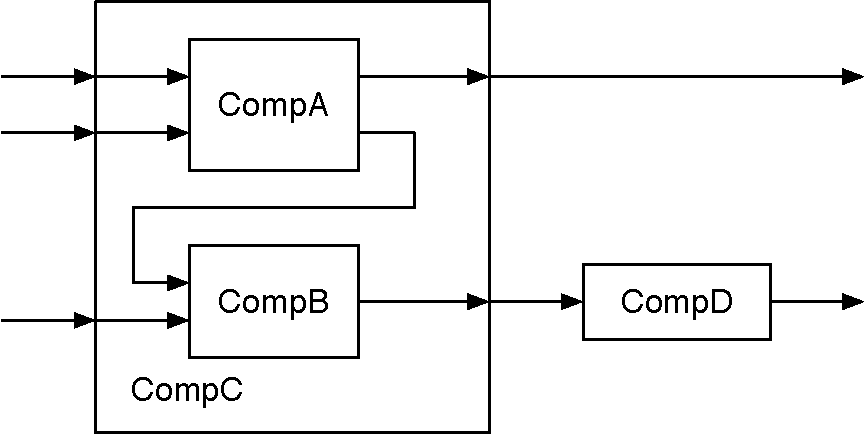
\includegraphics[scale=\scale]{figures/components}
  \caption{Một thiết kế gồm các thành phần phân cấp.}
  \label{fig:components}
\end{figure}

Một thiết kế mạch số lớn hơn được cấu trúc thành một tập hợp các thành phần, thường theo 
cách phân cấp. Mỗi thành phần có một giao tiếp với các dây ngõ vào và ngõ ra, thường được gọi là cổng. 
Chúng tương tự như các chân ngõ vào và ngõ ra trên mạch tích hợp (IC).
Các thành phần được kết nối với nhau bằng cách nối dây các ngõ vào và ngõ ra. 
Các thành phần có thể chứa các thành phần con để xây dựng hệ thống phân cấp.
Thành phần ngoài cùng, được kết nối với các chân vật lý trên chip, được gọi là thành phần cấp cao nhất (top-level).

Hình ~\ref{fig:components} biểu diễn một thiết kế ví dụ. Thành phần C có 
ba cổng ngõ vào và hai cổng ngõ ra. Bản thân thành phần này được ghép lại từ 
hai thành phần con: B và C, được kết nối với các ngõ vào và ngõ ra của C. 
Một ngõ ra của A được kết nối với ngõ vào của B. Thành phần D ở cùng cấp 
phân cấp với thành phần C và được kết nối với nó.

Trong chương này, chúng ta sẽ giải thích cách các thành phần được mô tả trong Chisel và 
cung cấp các ví dụ về các thành phần chuẩn. Các thành phần tiêu chuẩn đó phục vụ hai 
mục đích: (1) chúng cung cấp các ví dụ về mã Chisel và (2) chúng cung cấp một thư viện 
gồm các thành phần sẵn sàng được sử dụng lại trong thiết kế của các bạn.

\section{Các thành phần trong Chisel là mô-đun}

\index{Giao tiếp IO}

Các thành phần phần cứng được gọi là mô-đun trong Chisel. Mỗi mô-đun  mở rộng
lớp \code{Module} và chứa trường \code{io} cho việc giao tiếp.
Giao tiếp được định nghĩa bởi \code{Bundle} được gói thành một lệnh gọi đến \code{IO()}.
\code{Bundle} chứa các trường để biểu diễn các cổng ngõ vào và ngõ ra của mô-đun. 
Chỉ hướng vào ra được đưa ra bằng cách đưa một trường vào lệnh gọi \code{Input()} hoặc
\code{Output()}. Chỉ hướng là từ góc nhìn của chính thành phần đó.


\longlist{code/components_ab.txt}{Định nghĩa của thành phần A và B}{lst:comp:ab}

Listing~\ref{lst:comp:ab} biểu diễn định nghĩa của hai thành phần ví dụ A và B từ
Hình~\ref{fig:components}.
Thành phần A có hai ngõ vào, được đặt tên là \code{a} và \code{b}, và hai
ngõ ra, được đặt tên là \code{x} và \code{y}. Với những cổng của thành phần B
chúng ta chọn các tên là \code{in1}, \code{in2}, và \code{out}.
Tất cả các cổng sử dụng số nguyên không dấu (\code{UInt}) với độ rộng bit là 8.
Vì đoạn mã ví dụ này đề cập về kết nối các thành phần và xây dựng cấu trúc phân cấp, 
nên chúng ta không triển khai bất kỳ thực hiện nào trong các thành phần.
Việc triển khai thành phần được viết ở nơi các chú thích khai báo ``Hàm của X''.
Vì chúng ta không có hàm nào được liên kết với các thành phần của ví dụ này,
nên chúng ta sử dụng các tên cổng chung. Với một thiết kế thực sự, chúng ta sử dụng
các tên cổng mô tả, chẳng hạn như \code{data}, \code{valid}, hoặc \code{ready}.

Thành phần C, được biểu diễn trong Listing~\ref{lst:comp:c}, có ba cổng ngõ vào và hai ngõ ra.
Nó được xây dựng từ các thành phần A và B. Chúng ta chỉ ra cách A và B được kết nối với các cổng 
của C và cũng là kết nối giữa cổng ngõ ra của A và cổng ngõ vào của B.

\longlist{code/components_c.txt}{Thành phần C}{lst:comp:c}


Thành phần C được tạo bởi \code{new}, ví dụ: \code{new CompA()}, và cần được gói trong một lệnh
gọi tới \code{Module()}. Tham chiếu đến mô-đun đó được lưu trong biến cục bộ, trong ví dụ này là \code{val compA = Module(new CompA())}.

Với tham chiếu này, chúng ta có thể truy cập đến các cổng IO bằng cách xóa tham chiếu
trường \code{io} của mô-đun và các trường riêng lẻ của \code{Bundle} IO.

Thành phần đơn giản nhất trong thiết kế, như đã biểu diễn trong Listing~\ref{lst:comp:d},
chỉ có một cổng ngõ vào, được đặt tên là \code{in}, và một cổng ngõ ra được đặt tên là \code{out}.

\longlist{code/components_d.txt}{Thành phần D}{lst:comp:d}

Phần còn thiếu cuối cùng của thiết kế ví dụ là thành phần mức cao nhất (top-level), chính nó
được ghép nối từ các thành phần C và D, như được biểu diễn trong Listing~\ref{lst:comp:top}.

\longlist{code/components_top.txt}{Thành phần cao nhất}{lst:comp:top}

Thiết kế các thành phần tốt tương tự như việc thiết kế tốt các hàm hoặc phương pháp trong 
thiết kế phần mềm. Một trong những câu hỏi chính là chúng ta sẽ đưa bao nhiêu chức năng vào 
một thành phần và một thành phần phải lớn như thế nào. Có hai thái cực: các thành phần nhỏ chẳng hạn như mạch cộng 
và các thành phần khổng lồ chẳng hạn như một bộ vi xử lý đầy đủ.

Những người mới bắt đầu thiết kế phần cứng thường bắt đầu với các thành phần nhỏ. 
Vấn đề là sách thiết kế mạch số sử dụng các thành phần nhỏ để biểu diễn các nguyên lý. 
Nhưng kích thước của các ví dụ (trong những cuốn sách đó và cả trong cuốn sách này) nhỏ 
để vừa với một trang và không làm người đọc xao nhãng bởi quá nhiều chi tiết.

Với các thành phần nhỏ, như mạch đếm, Chisel cung cấp một cách nhẹ nhàng hơn 
để mô tả chúng như các hàm trả về phần cứng.

Giao tiếp với một thành phần hơi dài dòng một chút (với các kiểu, tên, 
hướng, cấu trúc IO). Theo nguyên tắc chung, tôi đề xuất rằng lõi của thành phần, 
của hàm, ít nhất phải dài bằng giao tiếp của thành phần.

\section{Đơn vị Logic số học}

Một trong những thành phần trung tâm của mạch điện tính toán, ví dụ như bộ vi xử lý, là
\myref{https://en.wikipedia.org/wiki/Arithmetic_logic_unit}{đơn vị logic số học},
hay ghi tắt là ALU. Hình~\ref{fig:alu} biểu diễn biểu tượng của một ALU.

\index{ALU}

\begin{figure}
  \centering
  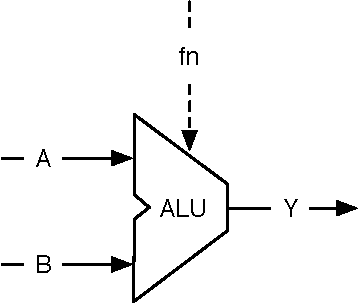
\includegraphics[scale=\scale]{figures/alu}
  \caption{Đơn vị logic số học, hoặc ghi tắt là ALU.}
  \label{fig:alu}
\end{figure}

ALU có hai ngõ vào, đặt nhãn là \code{A} và \code{B} như trong hình, một ngõ vào chức năng \code{fn},
và một ngõ ra, đặt nhãn là {Y}. ALU hoạt động dựa trên giá trị \code{A} và \code{B} và đưa kết quả ở ngõ ra. 
Ngõ vào \code{fn} chọn phép toán cho \code{A} và \code{B}.
Các phép toán thường là dạng số học, chẳng hạn như phép cộng và phép trừ, và một số phép toán
logic như and, or, xor. Đó là lý do tại sao nó được gọi là ALU.

Ngõ vào chức năng \code{fn} chọn phép toán. ALU thường là mạch tổ hợp không có bất kỳ phần tử trạng thái nào.
Một ALU còn có thể có ngõ ra bổ sung để báo hiệu các đặc tính của kết quả như cờ zero, cờ dấu.

Đoạn mã sau đây biểu diễn một ALU có ngõ vào và ngõ ra 16-bit hỗ trợ các phép toán: cộng, trừ, OR, AND và 
phép toán khác được chọn bởi tín hiệu \code{fn} 2-bit.

\shortlist{code/components_alu.txt}

\noindent Trong ví dụ này, chúng ta sử dụng một cấu trúc Chisel mới, cấu trúc \code{switch/is}, 
để mô tả bảng chọn ngõ ra của ALU. Để sử dụng chức năng tiện ích này, chúng ta cần nhập (import) một gói Chisel khác:

\shortlist{code/components_util.txt}

\section{Các kết nối khối}

\index{Kết nối khối}

Để kết nối các thành phần có nhiều cổng IO, Chisel cung cấp toán tử 
kết nối khối (bulk connection) \code{<>}. Toán tử này kết nối các phần của bundle theo cả hai hướng. 
Chisel sử dụng tên của các trường lá (leaf field) để kết nối. Nếu thiếu tên, nó không được kết nối.

Ví dụ, hãy giả sử chúng ta xây dựng một bộ xử lý đường ống (pipeline). Giai đoạn nạp lệnh có giao tiếp sau:

\shortlist{code/bundle_fetch.txt}

\noindent Giai đoạn tiếp theo là giai đoạn giải mã lệnh.
\shortlist{code/bundle_decode.txt}

\noindent Giai đoạn cuối cùng của bộ xử lý đơn giản của chúng ta là giai đoạn thực thi.
\shortlist{code/bundle_execute.txt}

Để kết nối tất cả ba giai đoạn, chúng ta cần hai toán tử \code{<>}.
Chúng ta cũng có thể kết nối cổng của mô-đun con với mô-đun mẹ.
\shortlist{code/bundle_connect.txt}


\section{Các thành phần nhẹ dùng các hàm}
\label{sec:functions}

\index{Các thành phần hàm}

Mô-đun là cách tổng quát để cấu trúc việc mô tả phần cứng của các bạn.
Tuy nhiên, có một số mã  code viết sẵn khi khai báo một mô-đun và khi khởi tạo và kết nối nó.
Một cách gọn nhẹ để cấu trúc phần cứng của các bạn là sử dụng các hàm.
Các hàm Scala có thể nhận các tham số Chisel (và Scala) và trả về phần cứng đã được tạo.
Với một ví dụ đơn giản, chúng ta tạo một mạch cộng:

\shortlist{code/components_fn_def.txt}

\noindent Chúng ta có thể tạo hai mạch cộng bằng cách đơn giản gọi hàm \code{adder}.

\shortlist{code/components_fn_use.txt}

\noindent Lưu ý rằng đây là \emph{bộ tạo phần cứng}. Các bạn không thực hiện bất kỳ thao tác thêm 
nào trong khi build, nhưng hãy tạo hai mạch cộng (thực thể phần cứng). Mạch cộng là một ví dụ nhân tạo đơn giản. 
Chisel đã có sẵn hàm tạo mạch cộng, chẳng hạn như \code{+(that: UInt)}.

Các hàm, như là bộ tạo phần cứng nhẹ, cũng có thể chứa trạng thái (bao gồm thanh ghi).
Ví dụ sau trả về một phần tử trễ một chu kỳ đồng hồ (một thanh ghi).
Nếu một hàm chỉ có một câu lệnh duy nhất, thì chúng ta có thể viết nó trong một dòng và bỏ qua dấu ngoặc ({}).

\shortlist{code/components_fn_delay.txt}

\noindent Bằng cách gọi hàm với chính hàm làm tham số, điều này tạo ra độ trễ hai chu kỳ xung clock.

\shortlist{code/components_fn_2delay.txt}

\noindent Một lần nữa, đây là một ví dụ rất ngắn nhưng hữu ích, vì \code{RegNext()} đã là hàm tạo thanh ghi cho độ trễ.

Các hàm có thể được khai báo như một phần của \code{Module}. Tuy nhiên, các hàm sẽ được 
sử dụng trong các mô-đun khác nhau  thì tốt hơn là được đặt trong một đối tượng Scala 
để lấy các hàm tiện ích.

\chapter{Các khối xây dựng mạch tổ hợp}

Trong chương này, chúng ta khám phá các mạch tổ hợp khác nhau, các khối xây dựng cơ bản mà 
chúng ta có thể sử dụng để xây dựng các hệ thống phức tạp hơn.
Về nguyên tắc, tất cả các mạch tổ hợp có thể được mô tả bằng phương trình đại số Boole.
Tuy nhiên, thông thường, mô tả dưới dạng bảng sẽ hiệu quả hơn.
Chúng ta sẽ để công cụ tổng hợp trích xuất và tối thiểu hóa các phương trình đại số Boole.
Hai mạch cơ bản, được mô tả tốt nhất dưới dạng bảng, là mạch giải mã và mạch mã hóa.

\section{Các mạch tổ hợp}

\index{Mạch tổ hợp}

Trước khi mô tả một số khối xây dựng mạch tổ hợp tiêu chuẩn, chúng ta sẽ khám phá 
cách các mạch tổ hợp có thể được biểu diễn trong Chisel.
Dạng đơn giản nhất là biểu thức đại số Boole, có thể được gán với một tên:

\shortlist{code/comb_bool.txt}

\noindent Biểu thức đại số Boole được đặt tên (\code{e}) bằng cách gán nó
với một giá trị Scala. Biểu thức có thể được tái sử dụng lại trong những biểu thức khác:

\shortlist{code/comb_use.txt}

Một biểu thức nhu vậy được xem như là cố định. Một phép gán lại cho \code{e}
bởi \code{=} sẽ dẫn đến lỗi trình biên dịch Scala: \code{reassignment to val}.
Chúng ta thử với toán tử Chisel \code{:=}, được biểu diễn như sau,

\shortlist{code/comb_error.txt}

\noindent sẽ dẫn đến một ngoại lệ runtime: \code{Cannot reassign to read-only}.

Chisel cũng hỗ trợ mô tả các mạch tổ hợp với các cập nhật có điều kiện.

Một mạch điện như vậy được khai báo là \code{Wire}. Sau đó, các bạn sử dụng các phép toán điều kiện,
như \code{when}, để mô tả logic của mạch điện.
Đoạn mã sau khai báo \code{Wire} \code{w} kiểu \code{UInt} và gán một giá trị mặc định 
\code{0}. Khối \code{when} kiểu \code{Bool} trong Chisel và gán lại giá trị
\code{3} cho \code{w} nếu giá trị của \code{cond} là \code{true.B}.

\shortlist{code/comb_wire.txt}

\noindent Logic mạch điện là mạch đa hợp, với hai ngõ vào là hằng số
\code{0} và \code{3} và tín hiệu chọn điều kiện \code{cond}.
Nên nhớ rằng chúng ta mô tả các mạch phần cứng chứ không phải chương trình phần mềm được thực thi có điều  kiện.

Cấu trúc điều kiện \code{when} trong Chisel còn có dạng \emph{else}, nó được gọi là
\code{otherwise}. Với việc gán giá trị trong bất kỳ điều kiện nào, chúng ta có thể bỏ qua việc gán giá trị mặc định:

\shortlist{code/comb_otherwise.txt}

\index{when}
\index{if/elseif/else}
\index{otherwise}
\index{elsewhen}

\begin{figure}
  \centering
  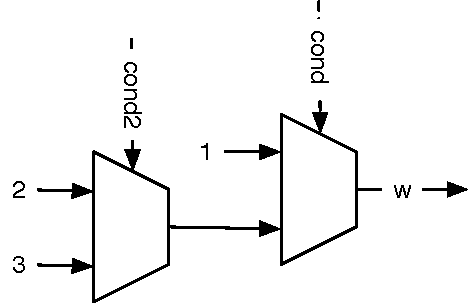
\includegraphics[scale=\scale]{figures/mux-chain}
  \caption{Chuỗi các mạch đa hợp.}
  \label{fig:mux-chain}
\end{figure}

Chisel còn hỗ trợ chuỗi các điều kiện (chuỗi if/elseif/else) với \code{.elsewhen}:

\shortlist{code/comb_elsewhen.txt}

\noindent Chuỗi \code{when}, \code{.elsewhen}, và \code{.otherwise}
tạo thành chuỗi các mạch đa hợp. Hình~\ref{fig:mux-chain} biểu diễn chuỗi các mạch đa hợp này.
Chuỗi đó đưa ra mức độ ưu tiên, ví dụ: khi \code{cond} là đúng, các điều kiện khác sẽ không được đánh giá.

Lưu ý `.' trong \code{.elsewhen} cần thiết với các phương pháp chuỗi trong Scala.
Những nhánh \code{.elsewhen} đó có thể dài ngẫu nhiên.
Tuy nhiên, nếu chuỗi điều kiện phụ thuộc vào một tín hiệu duy nhất, thì tốt hơn
là sử dụng lệnh \code{switch}, được giới thiệu trong phần sau với mạch giải mã. 

Đối với các mạch tổ hợp phức tạp hơn, thực tế là gán giá trị mặc định 
cho \code{Wire}. Phép gán mặc định có thể được kết hợp với khai báo đi dây với \code{WireDefault}.

\shortlist{code/comb_wiredefault.txt}

Người ta có thể đặt câu hỏi là tại sao lại sử dụng \code{when}, \code{.elsewhen} và \code{else} 
khi Scala có \code{if}, \code{else if} và \code{else}? Các câu lệnh đó là để thực thi 
có điều kiện mã Scala, không tạo ra phần cứng Chisel (mạch đa hợp).
Các điều kiện Scala đó có công dụng trong Chisel khi chúng ta viết các 
trình tạo mạch, lấy các tham số để tạo các thực thể phần cứng \emph{khác} một cách có điều kiện.

\section{Mạch giải mã}

\index{Mạch giải mã}

\myref{https://en.wikipedia.org/wiki/Binary_decoder}{Mạch giải mã}
đổi số nhị phân $n$ bits thành tín hiệu $m$-bit, với $m \leq 2^n$.
Ngõ ra được mã hóa one-hot (trong đó chính xác một bit bằng 1).

\begin{figure}
  \centering
  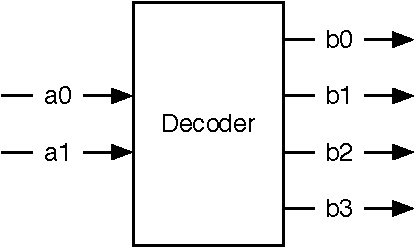
\includegraphics[scale=\scale]{figures/decoder}
  \caption{Mạch giải mã 2-bit ra 4-bit.}
  \label{fig:decoder}
\end{figure}

Hình~\ref{fig:decoder} biểu diễn mạch giải mã 2-bit ra 4-bit. Chúng ta có thể mô tả chức năng của 
mạch giải mã bằng bảng trạng thái, như Bảng~\ref{tab:decoder}.

\begin{table}
 \centering
 \label{tab:decoder}
  \begin{tabular}{rr}
    \toprule
    a & b \\
    \midrule
    00 & 0001 \\
    01 & 0010 \\
    10 & 0100 \\
    11 & 1000 \\
    \bottomrule 
  \end{tabular} 
  \caption{Bảng trạng thái cho mạch giải mã 2 ra 4.}
\end{table}

Câu lệnh Chisel \code{switch} mô tả logic dưới dạng bảng trạng thái.
Câu lệnh \code{switch} không phải là một phần của ngôn ngữ Chisel cốt lõi.
Vì vậy, chúng ta cần đưa vào các thành phần của gói \code{chisel.util}.

\shortlist{code/encdec_util.txt}

\noindent Đoạn mã sau giới thiệu lệnh \code{switch} của Chisel để mô tả mạch giải mã:

\index{switch}

\shortlist{code/encdec_dec.txt}

\noindent Câu lệnh \code{switch} ở trên liệt kê tất cả giá trị có thể có của tín hiệu \code{sel} 
và gán giá trị giải mã cho tín hiệu \code{result}.
Lưu ý rằng ngay cả khi chúng ta liệt kê tất cả các giá trị ngõ vào có thể có, Chisel vẫn cần 
chúng ta gán cho một giá trị mặc định, giống như chúng ta thực hiện bằng cách gán 0 cho \code{result}.
Việc gán này này sẽ không bao giờ kích hoạt và do đó được tối ưu hóa bởi công cụ đầu cuối (backend).
Nó nhằm tránh các tình huống có phép gán chưa hoàn tất cho các mạch tổ hợp 
(trong Chisel là \code{Wire}) sẽ dẫn đến các mạch chốt không mong muốn trong các ngôn ngữ mô tả 
phần cứng như VHDL và Verilog. Chisel không cho phép các phép gán chưa hoàn tất.

Trong ví dụ trước, chúng ta đã sử dụng số nguyên không dấu cho các tín hiệu. 
Một biểu diễn rõ ràng hơn của mạch mã hóa sử dụng ký hiệu nhị phân:

\shortlist{code/encdec_decbin.txt}

\todo{from Luca: for very small examples. What if the one-hot input is 256 wires? Can Chisel capture that? Or I need 256 lines? I would suggest to put an additional example. Maybe there is something like the for loop in VHDL.}

Một bảng cung cấp một biểu diễn rất dễ đọc của chức năng giải mã nhưng cũng hơi dài dòng.
Khi xem bảng, chúng ta thấy một cấu trúc thông thường: giá trị 1 được dịch sang trái bởi số được 
biểu diễn bởi \code{sel}. Do đó, chúng ta có thể biểu diễn một mạch giải mã bằng phép toán dịch trong Chisel \code{<<}.

\shortlist{code/encdec_shift.txt}

Mạch giải mã được sử dụng như một khối xây dựng cho mạch đa hợp bằng cách sử dụng ngõ ra 
là tín hiệu điều khiển với cổng AND cho ngõ vào dữ liệu của mạch đa hợp. Tuy nhiên, trong Chisel, 
chúng ta không cần phải xây dựng một mạch đa hợp, vì \code{Mux} có sẵn trong thư viện lõi.
Mạch giải mã cũng có thể được sử dụng để giải mã địa chỉ và sau đó các ngõ ra được sử dụng 
như các tín hiệu chọn, ví dụ: các linh kiện IO khác nhau được kết nối với bộ vi xử lý.

\section{Mạch giải mã}
\index{Mạch giải mã}

\myref{https://en.wikipedia.org/wiki/Encoder_(digital)}{Mạch mã hóa}
đổi tín hiệu ngõ vào one-hot thành tín hiệu ngõ ra được mã hóa nhị phân.
Mạch mã hóa hoạt động ngược lại với mạch giải mã.

\begin{figure}
  \centering
  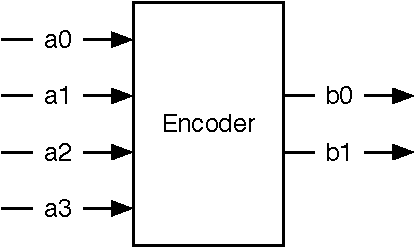
\includegraphics[scale=\scale]{figures/encoder}
  \caption{Mạch mã hóa 4-bit thành 2-bit.}
  \label{fig:encoder}
\end{figure}


\begin{table}
 \centering
 \label{tab:encoder}
  \begin{tabular}{rr}
    \toprule
    a & b \\
    \midrule
    0001 & 00 \\
    0010 & 01 \\
    0100 & 10 \\
    1000 & 11 \\
    ???? & ?? \\
    \bottomrule 
  \end{tabular} 
  \caption{Bảng trạng thái cho mạch mã hóa 4 thành 2.}
\end{table}

Hình~\ref{fig:encoder} biểu diễn mạch mã hóa ngõ vào 4-bit one-hot thành ngõ ra nhị phân 2-bit, 
và Bảng~\ref{tab:encoder} biểu diễn bảng trạng thái chức năng mã hóa. Tuy nhiên, mạch mã hóa chỉ 
hoạt động như mong đợi khi tín hiệu ngõ vào được mã hóa one-hot. Đối với tất cả các giá trị ngõ vào khác, 
giá trị ngõ ra là không xác định. Vì chúng ta không thể mô tả một hàm có ngõ ra không xác định, 
nên chúng ta sử dụng một phép gán mặc định để bắt tất cả các mẫu ngõ vào không xác định.

Mã Chisel sau gán giá trị mặc định là 00 và sau đó sử dụng câu lệnh switch cho các giá trị ngõ vào hợp lệ.

\shortlist{code/encdec_enc.txt}

\section{Bài tập}

Mô tả mạch tổ hợp để chuyển đổi ngõ vào nhị phân 4-bit thành giá trị mã hóa 
\myref{https://en.wikipedia.org/wiki/Seven-segment_display}{hiển thị LED 7-đoạn}.
Các bạn có thể định nghĩa mã cho các chữ số thập phân, đây là cách sử dụng để khởi tạo ban đầu của hiển thị 
LED 7-đoạn, hoặc bổ sung thêm định nghĩa mã cho các bit còn lại để có thể hiển thị tất cả 
16 giá trị của chữ số trong \myref{https://en.wikipedia.org/wiki/Hexadecimal}{hệ thập lục phân}.
Nếu bo mạch FPGA của các bạn có LED 7-đoạn, hãy kết nối ngõ vào của mạch với 4 công tắc gạt hoặc nút nhấn 
và nối ngõ ra với LED 7-đoạn.

\chapter{Các khối xây dựng mạch tuần tự}

Mạch tuần tự là mạch điện mà giá trị ngõ ra phụ thuộc vào giá trị ngõ vào \emph{và}
giá trị trước đó. Vì chúng ta quan tâm đến thiết kế đồng bộ (thiết kế có xung clock),
nên chúng ta muốn nói đến mạch tuần tự đồng bộ khi chúng ta nói về mạch tuần 
tự.\footnote{Chúng ta cũng có thể xây dựng các mạch tuần tự với logic và hồi tiếp 
bất đồng bộ, nhưng đây là một chủ đề cụ thể và không thể diễn đạt bằng Chisel.}
Để xây dựng các mạch tuần tự, chúng ta cần các phần tử có thể lưu trữ trạng thái: được gọi là thanh ghi.

\section{Các thanh ghi}

\index{Thanh ghi}
\index{Flip-flop}

\begin{figure}
  \centering
  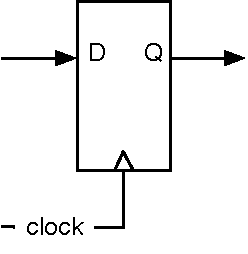
\includegraphics[scale=\scale]{figures/register}
  \caption{Thanh ghi dựa trên Flip-flop D.}
  \label{fig:register}
\end{figure}

Các thành phần cơ bản để xây dựng các mạch tuần tự là thanh ghi. Một thanh ghi là tập hợp gồm 
nhiều \myref{https://en.wikipedia.org/wiki/Flip-flop_(electronics)\#D_flip-flop}{flip-flop D}.
Một flip-flop D giữ lại giá trị ngõ vào của nó ở cạnh lên của xung clock và lưu trữ nó ở ngõ ra. 
Ngoài ra, nói cách khác: thanh ghi cập nhật giá trị ngõ ra của nó với giá trị của ngõ vào ở cạnh lên của xung clock.

\index{Xung clock}
Hình~\ref{fig:register} biểu diễn biểu tượng trong sơ đồ mạch điện của thanh ghi. Nó chứa ngõ vào
\code{D} và ngõ ra \code{Q}. Mỗi thanh ghi còn chứa tín hiệu ngõ vào \code{clock}.
Vì tín hiệu xung clock toàn cục này được kết nối với tất cả các thanh ghi trong mạch đồng bộ, nên nó thường 
không được vẽ trong sơ đồ mạch điện. Hình tam giác nhỏ ở dưới tượng trưng cho ngõ vào xung clock và 
cho chúng ta biết rằng đây là một thanh ghi. Chúng ta bỏ qua tín hiệu xung clock trong các sơ đồ mạch điện sau.
Việc bỏ qua tín hiệu xung clock toàn cục cũng được phản ánh trong Chisel khi không cần có kết nối rõ ràng tín hiệu với 
ngõ vào xung clock của thanh ghi.

Trong Chisel, một thanh ghi với ngõ vào \code{d} và ngõ ra \code{q} được định nghĩa bởi:

\shortlist{code/sequ_reg.txt}

\noindent Lưu ý rằng chúng ta không cần kết nối xung clock với thanh ghi, Chisel đã 
ngầm thực hiện điều này. Ngõ vào và ngõ ra của thanh ghi có thể là các kiểu phức tạp 
tùy ý được tạo ra từ sự kết hợp của các véc-tơ và các bundle.

Một thanh ghi cũng có thể được định nghĩa và sử dụng theo hai bước:

\shortlist{code/sequ_reg2.txt}

Đầu tiên, chúng ta định nghĩa thanh ghi và cho nó một cái tên. Thứ hai, chúng ta kết 
nối tín hiệu \code{delayIn} với ngõ vào của thanh ghi. Cũng lưu ý rằng tên của thanh ghi 
chứa chuỗi \code{Reg}. Để dễ dàng phân biệt giữa mạch tổ hợp và mạch tuần tự, thông thường 
chúng ta sử dụng nhãn \code{Reg} như một phần của tên. Ngoài ra, lưu ý rằng các tên 
trong Scala (và do đó cũng trong Chisel) thường ở là
\myref{https://en.wikipedia.org/wiki/Camel_case}{CamelCase}.
Tên biến bắt đầu bằng chữ thường và các lớp bắt đầu bằng chữ hoa.

\index{Reset}
\index{Khởi tạo}
Một thanh ghi cũng có thể được khởi tạo khi reset. Tín hiệu \code{reset}, giống như tín hiệu \code{clock}, 
ẩn chứa trong Chisel. Chúng ta cung cấp giá trị cho reset, ví dụ là 0, như là tham số cho bộ 
tạo thanh ghi \code{RegInit}. Ngõ vào cho thanh ghi được kết nối với một lệnh gán trong Chisel.

\shortlist{code/sequ_reg_init.txt}

Việc thực hiện mặc định reset trong Chisel là reset đồng bộ\footnote{Hỗ trợ cho reset bất đồng bộ 
hiện đang được phát triển}. Với reset đồng bộ, không cần thay đổi trên flip-flop D, chỉ cần thêm mạch đa 
hợp\footnote{Các flip-flop trong FPGA hiện tại chứa ngõ vào reset đồng bộ.
Do đó, không cần thêm tài nguyên nào cho mạch đa hợp.} vào ngõ vào để chọn 
giữa giá trị khởi tạo khi reset và giá trị dữ liệu.

\begin{figure}
  \centering
  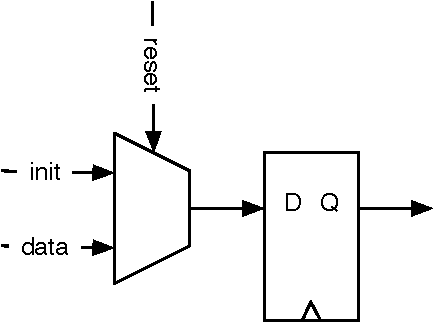
\includegraphics[scale=\scale]{figures/register-reset}
  \caption{Thanh ghi dựa trên flip-flop D với reset đồng bộ.}
  \label{fig:register-reset}
\end{figure}

Hình~\ref{fig:register-reset} biểu diễn sơ đồ mạch điện của một thanh ghi với reset đồng bộ 
trong đó reset sẽ điều khiển mạch đa hợp. Tuy nhiên, vì reset đồng bộ được sử dụng khá thường 
xuyên, nên các flip-flop FPGA hiện đại chứa ngõ vào reset (và set) đồng bộ để không lãng phí tài 
nguyên LUT cho mạch đa hợp.

Các mạch tuần tự thay đổi giá trị của chúng theo thời gian. Do đó, hành vi của chúng có thể được 
mô tả bằng một biểu đồ hiển thị các tín hiệu theo thời gian. Biểu đồ như vậy được gọi là dạng sóng 
\myref{https://en.wikipedia.org/wiki/Digital_timing_diagram}{biểu đồ thời gian}.

\index{Biểu đồ thời gian}
\index{Biểu đồ dạng sóng}

\todo{from Luca: Do readers know about timing diagrams?}

\begin{figure}
  \centering
  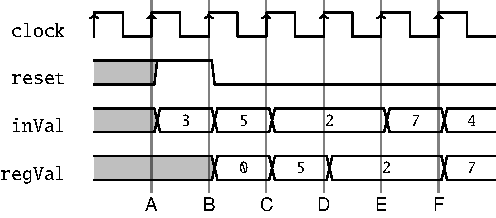
\includegraphics[scale=1]{figures/reg_wave}
  \caption{Dạng sóng của thanh ghi với tín hiệu reset.}
  \label{fig:register-wave}
\end{figure}

Hình~\ref{fig:register-wave} biểu diễn dạng sóng của thanh ghi với tín hiệu reset
và một số dữ liệu ngõ vào được áp vào nó.
Thời gian tăng dần từ trái sang phải. Ở phía trên hình, chúng ta thấy xung clock điều khiển mạch điện. 
Trong chu kỳ xung clock đầu tiên, trước khi reset, nội dung thanh ghi là không xác định. Trong chu kỳ đồng hồ thứ hai, 
reset được đưa lên ở mức cao và ở cạnh lên của chu kỳ xung clock này (được gán nhãn B), thanh ghi nhận giá trị 
ban đầu \code{0}. Ngõ vào \code{inVal} bị bỏ qua. Trong chu kỳ xung clock tiếp theo, \code{reset} 
bằng \code{0} và giá trị của \code{inVal} được ghi lại ở cạnh lên tiếp theo (được gán nhãn C). 
Từ đó trở đi \code{reset} vẫn giữ nguyên giá trị là \code{0}, và ngõ ra thanh ghi đi sau tín hiệu ngõ vào với độ trễ một chu kỳ xung clock.

Dạng sóng là một công cụ tuyệt vời để xác định hành vi của mạch bằng đồ họa. 
Đặc biệt là trong các mạch phức tạp hơn, nơi nhiều phép toán tiến hành song song và 
dữ liệu di chuyển theo đường ống (pipeline) xuyên suốt mạch, biểu đồ thời gian trở nên thuận tiện.
Các trình kiểm tra Chisel cũng có thể tạo ra các dạng sóng trong quá trình kiểm tra, dạng sóng có 
thể được hiển thị bằng công cụ xem dạng sóng và được sử dụng để gỡ lỗi.

Một mẫu thiết kế tiêu biểu là một thanh ghi có tín hiệu cho phép. Chỉ khi tín hiệu 
cho phép là \code{true} (mức cao), thanh ghi mới giữ lại giá trị ngõ vào; ngược lại, nó vẫn giữ nguyên giá trị cũ.
Tín hiệu cho phép có thể được thực hiện, tương tự như tín hiệu reset đồng bộ, với một mạch đa hợp ở ngõ 
vào của thanh ghi. Một ngõ vào cho mạch đa hợp là hồi tiếp ngõ ra của thanh ghi.
\index{Thanh ghi!tín hiệu cho phép}

\begin{figure}
  \centering
  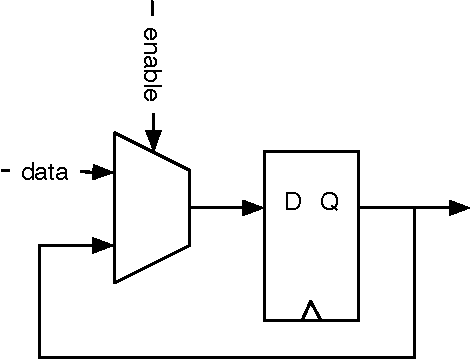
\includegraphics[scale=\scale]{figures/register-enable}
  \caption{Thanh ghi dựa trên flip-flop D vói tín hiệu cho phép.}
  \label{fig:register-enable}
\end{figure}

Hình~\ref{fig:register-enable} biểu diễn sơ đồ mạch điện của một thanh ghi có tín hiệu cho phép.
Vì đây cũng là một mẫu thiết kế phổ biến, các flip-flop trong FPGA hiện đại chứa ngõ vào cho phép 
dành riêng và không cần thêm tài nguyên.

\begin{figure}
  \centering
  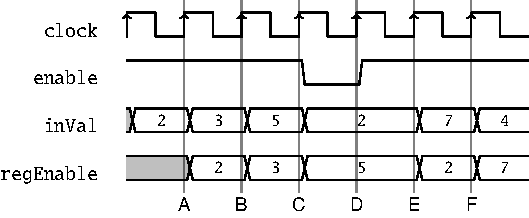
\includegraphics[scale=1]{figures/reg_en_wave}
  \caption{Biểu đồ dạng sóng của thanh ghi với tín hiệu cho phép.}
  \label{fig:register-en-wave}
\end{figure}

Hình~\ref{fig:register-en-wave} biểu diễn một dạng sóng ví dụ cho thanh ghi có tín hiệu cho phép. 
Hầu hết thời gian, bật tín hiệu cho phép ở mức cao (\code{true}) và thanh ghi 
đi sau ngõ vào với độ trễ một chu kỳ xung clock. Chỉ trong chu kỳ xung clock thứ tư, \code{enable} ở 
mức thấp, và thanh ghi giữ giá trị của nó (giá trị bằng 5) ở cạnh lên của nhãn D.

Thanh ghi với tín hiệu cho phép có thể được mô tả trong một vài dòng của mã Chisel với bản cập nhật có điều kiện:

\shortlist{code/sequ_reg_ena.txt}

\noindent Thanh ghi với tín hiệu cho phép có thể được reset:

\shortlist{code/sequ_reg_init_ena.txt}

Thanh ghi cũng có thể là một phần của một biểu thức. Mạch điện sau đây dò cạnh lên của tín hiệu 
bằng cách so sánh giá trị hiện tại của nó với giá trị từ chu kỳ xung clock sau cùng.

\shortlist{code/sequ_reg_rising.txt}

Bây giờ chúng ta đã khám phá tất cả các cách sử dụng cơ bản của một thanh ghi, chúng ta sử dụng tốt các thanh ghi đó 
và xây dựng các mạch tuần tự thú vị hơn.

\section{Mạch đếm}
\label{sec:counter}
\index{Mạch đếm}

\begin{figure}
  \centering
  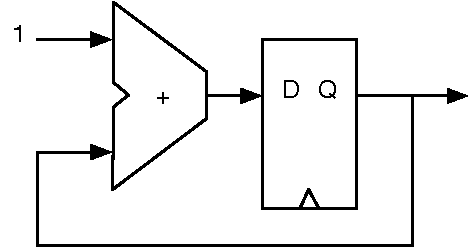
\includegraphics[scale=\scale]{figures/counter}
  \caption{Mạch cộng và kết quả thanh ghi trong mạch đếm.}
  \label{fig:counter}
\end{figure}

Một trong những mạch tuần tự cơ bản nhất là mạch đếm. Ở dạng đơn giản nhất, mạch đếm là một thanh ghi 
nơi mà ngõ ra được kết nối với một mạch cộng và ngõ ra của mạch cộng được kết nối với ngõ vào của thanh 
ghi. Hình~\ref{fig:counter} biểu diễn một mạch đếm chạy tự do (free-running counter).

Mạch đếm chạy tự do có một thanh ghi 4-bit đếm từ 0 đến 15 và sau đó lại quay về 0 chạy tiếp. 
Một mạch đếm cũng phải được reset về một giá trị đã biết.

\shortlist{code/sequ_free_counter.txt}

\begin{figure}
  \centering
  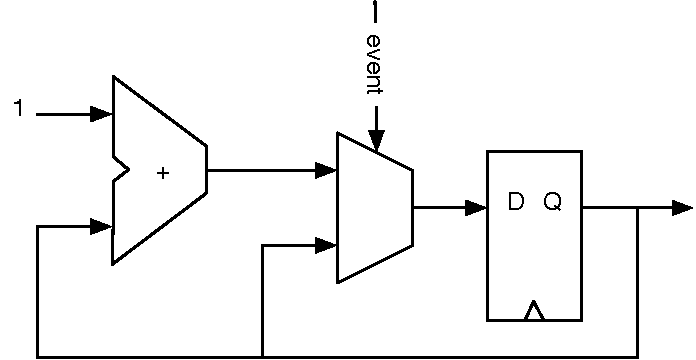
\includegraphics[scale=\scale]{figures/event-counter}
  \caption{Các sự kiện đếm.}
  \label{fig:event-counter}
\end{figure}

\noindent Khi chúng ta muốn đếm các sự kiện, chúng ta sử dụng một điều kiện để tăng giá trị cho mạch đếm, 
như trong Hình~\ref{fig:event-counter} và trong đoạn mã sau.

\shortlist{code/sequ_event_counter.txt}

\subsection{Đếm lên và đếm xuống}

Để đếm lên một giá trị và sau đó khởi động lại với giá trị \code{0}, chúng ta cần so sánh 
giá trị mạch đếm với một giá trị hằng số tối đa, ví dụ: với câu lệnh điều kiện \code{when}.

\shortlist{code/when_counter.txt}

\noindent Chúng ta còn có thể sử sụng mạch đa hợp cho mạch đếm:

\shortlist{code/mux_counter.txt}

\noindent Nếu đang ở trạng thái đếm xuống, thì chúng ta bắt đầu bằng cách đặt lại thanh ghi mạch đếm với giá trị cực đại và reset mạch đếm về giá trị đó khi đạt giá trị 0.

\shortlist{code/down_counter.txt}

\noindent Khi chúng ta đang viết mã code và sử dụng nhiều mạch đếm hơn, chúng ta có thể định nghĩa một hàm với một tham số để sinh tạo mạch đếm cho chúng ta. 

\shortlist{code/function_counter.txt}

\noindent Câu lệnh cuối cùng của hàm \code{genCounter} là giá trị trả về 
của hàm, trong ví dụ này là thanh ghi đếm \code{cntReg}.

Lưu ý rằng trong tất cả các ví dụ, mạch đếm có các giá trị giữa \code{0} và
\code{N}, bao gồm \code{N}. Nếu chúng ta muốn đếm 10 chu kỳ xung clock, chúng ta cần
đặt \code{N} là 9. Đặt \code{N} bằng 10 là ví dụ cổ điển về
\myref{https://en.wikipedia.org/wiki/Off-by-one_error}{lỗi logic off-by-one}.

\subsection{Tạo thời gian với mạch đếm}
\label{sec:gen:timing}

\index{Tạo thời gian}

Bên cạnh việc đếm các sự kiện, mạch đếm thường được sử dụng để tạo ra khái niệm về thời gian (thời gian giống như thời gian trên đồng hồ treo tường).
Mạch điện đồng bộ chạy với xung clock đồng hồ có tần số cố định.
Mạch sẽ hoạt động trong những thời điểm ứng với chu kỳ xung clock này. Không có khái niệm thời gian trong mạch số ngoài việc đếm các thời điểm với xung clock. Nếu chúng ta biết tần số xung clock, chúng ta có thể sinh ra các mạch tạo các sự kiện định thời, chẳng hạn như nhấp nháy đèn LED ở một số tần số như đã trình bày trong ví dụ ``Hello World''. 

Một thực tế phổ biến là để tạo một chu kỳ đơn \emph{tick} với tần số $f_{tick}$ mà chúng ta cần nó trong mạch của mình. Tín hiệu tick đó xảy ra sau mỗi $n$ chu kỳ xung clock, trong đó $n = f_{clock}/f_{tick}$ và tick có độ dài chính xác một chu kỳ xung clock.
Tín hiệu tick này \emph{không} được sử dụng như một xung clock được dẫn xuất, nhưng là một tín hiệu cho phép các thanh ghi trong mạch sẽ hoạt động hợp lý ở tần số $f_{tick}$.
Hình~\ref{fig:tick-wave} biểu diễn một ví dụ về một tín hiệu tick được tạo ra sau mỗi 3 chu kỳ xung clock. 

\begin{figure}
  \centering
  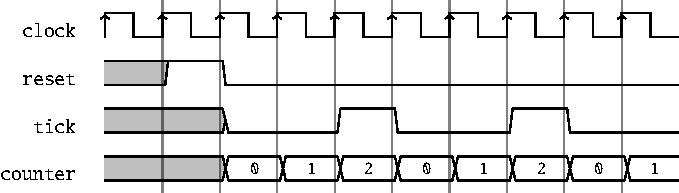
\includegraphics[scale=1]{figures/tick_wave}
  \caption{Sơ đồ dạng sóng để tạo một tick tần số chậm.}
  \label{fig:tick-wave}
\end{figure}


Trong mạch điện sau, chúng ta mô tả một mạch đếm sẽ đếm từ \code{0}
đến giá trị cực đại \code{N - 1}. Khi đạt đến giá trị cực đại,
\code{tick} là \code{true} cho một chu kỳ đơn, và mạch đếm được reset về \code{0}.
Khi chúng ta đếm từ \code{0} đến \code{N - 1}, chúng ta tạo một tick hợp lý mỗi chu kỳ xung clock \code{N}.

\shortlist{code/sequ_tick_gen.txt}

\index{Tick}
\noindent Thời gian logic của một tick với mỗi $n$ chu kỳ xung clock sau đó có thể được sử dụng để cải tiến các phần khác của mạch với xung clock logic chậm hơn này. Trong đoạn mã sau, chúng ta chỉ sử dụng một mạch đếm khác tăng dần lên \code{1} sau mỗi $n$ chu kỳ xung clock. 

\shortlist{code/sequ_tick_counter.txt}

\begin{figure}
  \centering
  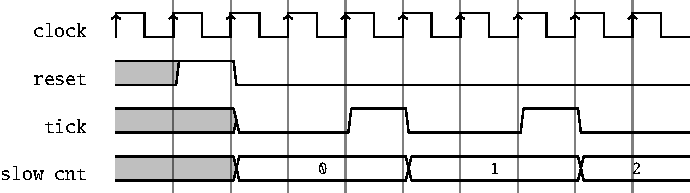
\includegraphics[scale=1]{figures/tick_count_wave}
  \caption{Sử dụng tick tần số chậm.}
  \label{fig:tick-count-wave}
\end{figure}

\noindent Hình~\ref{fig:tick-count-wave} biểu diễn dạng sóng của tín hiệu tick và mạch đếm chậm tăng lên mỗi tick ($n$ clock cycles).

\index{Xung clock logic}
Ví dụ về việc sử dụng xung clock \emph{logic} chậm hơn này là: nhấp nháy đèn LED, tạo tốc độ baud (baud rate) cho bus nối tiếp, tạo tín hiệu cho đa hợp hiển thị LED 7 đoạn và lấy mẫu con các giá trị ngõ vào để chống dội các nút và công tắc.

Mặc dù suy luận về giá trị độ rộng sẽ hình thành kích thước các thanh ghi, nhưng tốt hơn nên chỉ định rõ ràng giá trị độ rộng với kiểu khi định nghĩa thanh ghi hoặc với giá trị khởi tạo. Định nghĩa giá trị độ rộng rõ ràng có thể tránh được những bất ngờ khi giá trị reset của \code {0.U} dẫn đến kết quả mạch đếm có độ rộng là một bit. 

\subsection{Mạch đếm Nerd}

Đôi khi, nhiều người trong chúng ta cảm thấy mình giống như một \myref{https://en.wikipedia.org/wiki/Nerd}{người chú tâm về một vấn đề nào đó (nerd)}.
Ví dụ: chúng ta muốn thiết kế một phiên bản tối ưu hóa cao cho việc tạo mạch đếm/tick.
Một mạch đếm chuẩn cần các tài nguyên sau: một thanh ghi, một mạch cộng (hoặc mạch trừ) và một mạch so sánh. Chúng ta không thể làm gì nhiều về thanh ghi hoặc mạch cộng. Nếu đếm lên, chúng ta cần so sánh với một số, đó là một chuỗi bit. Mạch so sánh có thể được xây dựng từ các cổng đảo cho các số 0 trong chuỗi bit và một cổng AND lớn.
Khi đếm xuống đến 0, mạch so sánh là một cổng NOR lớn, có thể đơn giản hơn mạch so sánh một chút với một hằng số trong ASIC.
Trong FPGA, nơi cổng logic được xây dựng từ các bảng tra, không có sự khác biệt giữa việc so sánh với 0 hoặc 1. Yêu cầu về tài nguyên là như nhau đối với mạch đếm lên và đếm xuống.

Tuy nhiên, vẫn còn một mẹo nữa mà một nhà thiết kế phần cứng thông minh có thể thực hiện.
Cho đến nay, đếm lên hoặc đếm xuống cần phải so sánh với tất cả các bit đếm.
Điều gì sẽ xảy ra nếu chúng ta đếm từ N-2 xuống -1? Một số âm có bit MSB (Most Significant Bit) được đặt thành 1 và một số dương với bit này được đặt thành 0. Chúng ta chỉ cần kiểm tra bit này để phát hiện rằng mạch đếm của chúng ta đạt đến -1 hay chưa. Ở đây, mạch đếm được tạo bởi một nerd: 

\shortlist{code/nerd_counter.txt}


\subsection{Bộ định thời}

Một dạng định thời khác mà chúng ta có thể tạo, là bộ định thời one-shot. Bộ định thời one-shot cũng giống như bộ định thời trong nhà bếp: các bạn đặt số phút và nhấn nút bắt đầu. Khi hết khoảng thời gian được chỉ định, âm báo sẽ phát ra.
Bộ định thời kỹ thuật số được nạp với thời gian theo chu kỳ xung clock.
Sau đó, nó đếm xuống cho đến khi đạt đến giá trị 0. Ở giá trị 0, bộ định thời xác nhận với tín hiệu \emph{done}. 

Hình~\ref{fig:timer} biểu diễn sơ đồ khối của một bộ định thời. Thanh ghi có thể được nạp với
giá trị \code{din} bởi tín hiệu xác nhận \code{load}. Khi tín hiệu \code{load} không được xác nhận,
việc đếm xuống được lựa chọn (bằng cách chọn \code{cntReg - 1} như ngõ vào cho thanh ghi).
Khi mạch đếm đạt giá trị \code{0}, tín hiệu \code{done} được xác nhận và mạch đếm dừng đếm
bằng cách chọn ngõ vào của mạch đa hợp cung cấp giá trị \code{0}.

\begin{figure}
  \centering
  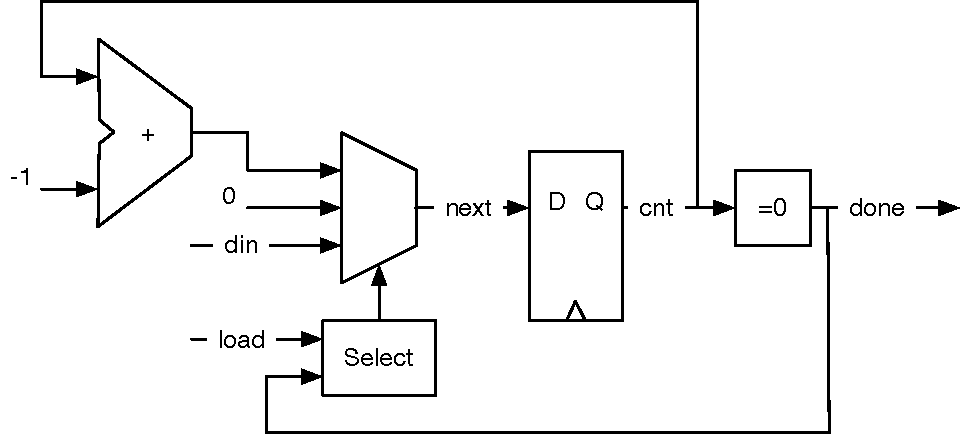
\includegraphics[scale=\scale]{figures/timer}
  \caption{Bộ định thời one-shot.}
  \label{fig:timer}
\end{figure}

Listing~\ref{lst:timer} biểu diễn mã Chisel cho bộ định thời. Chúng ta sử dụng một thanh ghi 8-bit \code{reg},
được reset về \code{0}. Giá trị boolean \code{done} là kết quả của việc so sánh \code{reg}
với \code{0}. Đối với mạch đa hợp ngõ vào, chúng ta đưa vào dây nối trung gian \code{next} với giá trị 
mặc định là \code{0}. Khối \code{when/elsewhen} đưa vào hai ngõ vào khác với chức năng lựa chọn tín hiệu. 
Tín hiệu \code{load} có mức độ ưu tiên qua độ lựa chọn giảm dần.
Dòng cuối cùng kết nối mạch đa hợp, được biểu diễn bởi \code{next}, với ngõ vào của thanh ghi \code{reg}. 

\longlist{code/timer.txt}{Bộ định thời one-shot}{lst:timer}

Nếu chúng ta nhắm đến mã chương trình ngắn gọn hơn một chút, thì chúng ta có thể gán trực tiếp các 
giá trị của mạch đa hợp cho thanh ghi \code{reg}, thay vì sử dụng dây trung gian \code{next}. 

\subsection{Điều biến độ rộng xung}

\myref{https://en.wikipedia.org/wiki/Pulse-width_Modulation}{Điều biến độ rộng xung} (Pulse-width modulation - PWM)
là tín hiệu có chu kỳ không đổi và điều biến thời gian tín hiệu là \emph{mức cao} trong chu kỳ đó.

\begin{figure}
  \centering
  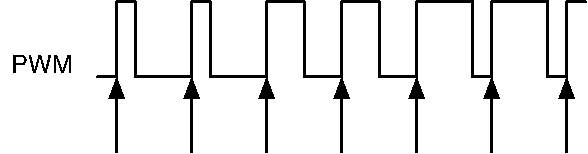
\includegraphics[scale=\scale]{figures/pwm}
  \caption{Điều biến độ rộng xung.}
  \label{fig:pwm}
\end{figure}

Hình~\ref{fig:pwm} biểu diễn một tín hiệu PWM. Các mũi tên trỏ đến điểm bắt đầu các 
khoảng thời gian của tín hiệu. Phần trăm thời gian tín hiệu ở mức cao, còn được gọi là 
chu kỳ nhiệm vụ (duty cycle). Trong hai chu kỳ đầu tiên, chu kỳ nhiệm vụ là 25\,\%, 
trong hai chu kỳ tiếp theo 50\,\%, và trong hai chu kỳ cuối là 75\,\%. Độ rộng xung được 
điều biến giữa 25\,\% và 75\,\%.

Thêm một \myref{https://en.wikipedia.org/wiki/Low-pass_filter}{mạch lọc thấp qua} vào tín hiệu PWM
sẽ cho ra một 
\myref{https://en.wikipedia.org/wiki/Digital-to-analog_converter}{bộ chuyển đổi số sang tương tự} đơn giản.
Mạch lọc thấp qua có thể ở dạng đơn giản chỉ với điện trở và tụ điện.

Ví dụ đoạn mã chương trình sau sẽ tạo dạng sóng 3 chu kỳ xung clock mức cao mỗi 10 chu kỳ xung clock.

\shortlist{code/pwm.txt}

\noindent Chúng ta sử dụng hàm cho bộ tạo PWM để cung cấp một thành phần nhẹ, tái sử dụng được.
Hàm có hai tham số: một số nguyên Scala cấu hình PWM với số chu kỳ xung clock (\code{nrCycles}), 
và một dây nối Chisel (\code{din}) để cung cấp giá trị chu kỳ nhiệm vụ (pulswidth) cho 
tín hiệu ngõ ra PWM. Chúng ta sử dụng một mạch đa hợp trong ví dụ này để biểu diễn mạch đếm.
Dòng cuối cùng của hàm: so sánh giá trị mạch đếm với giá trị ngõ vào \code{din} để trả về tín hiệu PWM. 
Biểu thức cuối cùng trong hàm là giá trị trả về, trong trường hợp của chúng ta, dây được nối với hàm so sánh.

Chúng ta sử dụng hàm \code{unsignedBitLength(n)} để xác định số bit cho mạch đếm
\code{cntReg} cần để biểu diễn các số không dấu lên đến (và bao gồm)
\code{n}.\footnote{Số bit để biểu diễn một số không dấu $n$ ở dạng nhị phân là $\lfloor log_2(n) \rfloor + 1$.}
Chisel còn có hàm \code{signedBitLength} để cung cấp số bit nhằm biểu diễn cho một số có dấu.


Một ứng dụng khác là sử dụng PWM để làm mờ đèn LED. Trong trường hợp đó, mắt đóng vai trò 
như bộ lọc thông thấp. Chúng ta mở rộng ví dụ trên để hướng quá trình tạo PWM bằng một hàm 
tam giác. Kết quả là một đèn LED có cường độ sáng thay đổi liên tục. 

\shortlist{code/pwm_modulate.txt}

Chúng ta sử dụng hai thanh ghi cho điều biến: (1) \code{modulationReg} để đếm lên và đếm xuống
và (2) \code{upReg} như cờ để xác định là đếm lên hay đếm xuống. Chúng ta đếm lên tần số
ngõ vào xung clock (100\,MHz trong ví dụ), cho ra kết quả tín hiệu
0.5\,Hz. Độ dài biểu thức \code{when/.elsewhen/.otherwise} xử lý việc đếm lên hay đếm xuống 
và chuyển hướng.

Vì PWM chỉ đếm lên đến phần 1000 của tần số để tạo ra tín hiệu 1\,kHz, 
chúng ta cần chia tín hiệu điều biến cho 1000. Vì phép chia số thực rất tốn kém trong phần cứng, 
chúng ta chỉ đơn giản dịch 10 lần sang phải, điều này tương đương một phép chia cho $2^{10} = 1024$.
Vì chúng ta đã định nghĩa mạch điện PWM như một hàm, nên có thể đơn giản khởi tạo mạch điện đó bằng cách 
gọi hàm. Dây nối \code{sig} biểu diễn tín hiệu PWM đã được điều biến. 

\section{Thanh ghi dịch}

\begin{figure}
  \centering
  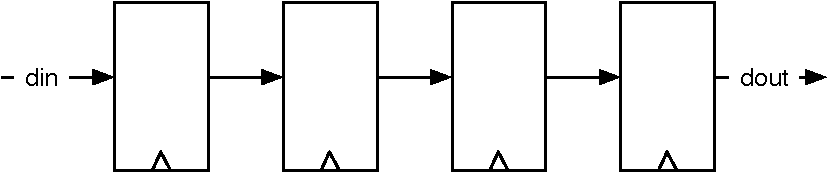
\includegraphics[scale=\scale]{figures/shiftregister}
  \caption{Thanh ghi dịch 4 tầng.}
  \label{fig:shiftregister}
\end{figure}


\myref{https://en.wikipedia.org/wiki/Shift_register}{Thanh ghi dịch} là tập hợp của các flip-flop
được kết nối thành một chuỗi. Mỗi ngõ ra của một thanh ghi (flip-flop) được nối với ngõ vào của 
thanh ghi kế tiếp. Hình~\ref{fig:shiftregister} biểu diễn thanh ghi dịch 4 tầng.
Mạch điện \emph{dịch} dữ liệu từ trái sang phải ở mỗi tick xung clock. Trong dạng đơn giản này,
mạch điện thực hiện độ trễ 4 lần từ \code{din} đến \code{dout}.

Mã Chisel cho thanh ghi dịch đơn giản này thực hiện: (1) tạo một thanh ghi 4-bit \code{shiftReg}, 
(2) ghép nối 3-bit thấp của thanh ghi dịch với ngõ vào \code{din} cho ngõ vào tiếp theo vào thanh ghi 
và (3) sử dụng bit MSB (Most Significant Bit) của thanh ghi làm ngõ ra \code{dout}. 

\shortlist{code/shift_register.txt}

Thanh ghi dịch thường được sử dụng để chuyển đổi dữ liệu từ nối tiếp sang song song hoặc dữ liệu từ song song sang nối tiếp. Phần~\ref{sec:uart} trình bày cổng nối tiếp sử dụng các thanh ghi dịch dùng cho chức năng nhận và gửi dữ liệu.

\subsection{Thanh ghi dịch với ngõ ra song song}

Cấu hình vào-nối-tiếp ra-song-song của thanh ghi dịch chuyển đổi dòng dữ liệu ngõ vào nối tiếp thành các từ song song. 
Điều này có thể được sử dụng trong cổng nối tiếp (UART) cho chức năng nhận dữ liệu. 
Hình~\ref{fig:shiftreg-paraout} biểu diễn thanh ghi dịch 4-bit, trong đó mỗi ngõ ra flip-flop
được nối với một bit ngõ ra. Sau 4 chu kỳ xong clock, mạch điện chuyển một từ (word) với 4-bit dữ liệu nối tiếp
thành một từ với 4-bit dữ liệu song song có sẵn trong \code{q}. Trong ví dụ này, chúng ta giả sử bit 0
(LSB) được gửi trước và do đó nó đến ở tầng cuối cùng khi chúng ta muốn đọc toàn bộ từ.

Trong đoạn mã Chisel sau, chúng ta khởi tạo thanh ghi dịch \code{outReg} với giá trị 0. Sau đó chúng ta dịch vào từ bit
MSB, có nghĩa là dịch phải. Kết quả song song, \code{q}, chỉ là việc đọc giá trị thanh ghi \code{outReg}.

\shortlist{code/shift_paraout.txt}

\begin{figure}
  \centering
  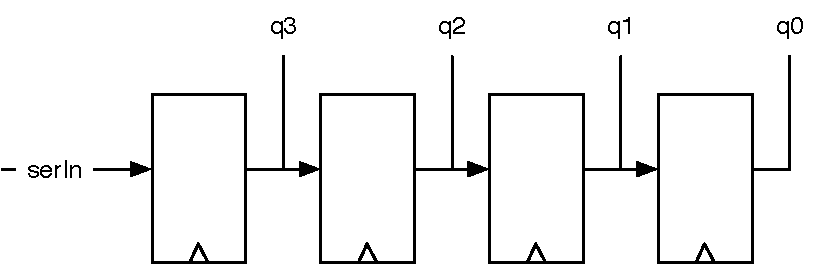
\includegraphics[scale=\scale]{figures/shiftreg-paraout}
  \caption{Thanh ghi dịch 4-bit với ngõ ra song song.}
  \label{fig:shiftreg-paraout}
\end{figure}

\noindent Hình~\ref{fig:shiftreg-paraout} biểu diễn thanh ghi dịch 4-bit với hàm ngõ ra song song.

\subsection{Thanh ghi dịch với tải song song}

Cấu hình vào-song-song ra-nối-tiếp của thanh ghi dịch chuyển đổi dòng dữ liệu các từ (bytes) ngõ vào song song thành dòng dữ liệu ngõ ra nối tiếp. 
Điều này có thể được sử dụng trong cổng nối tiếp (UART) cho chức năng gửi dữ liệu. 

\begin{figure}
  \centering
  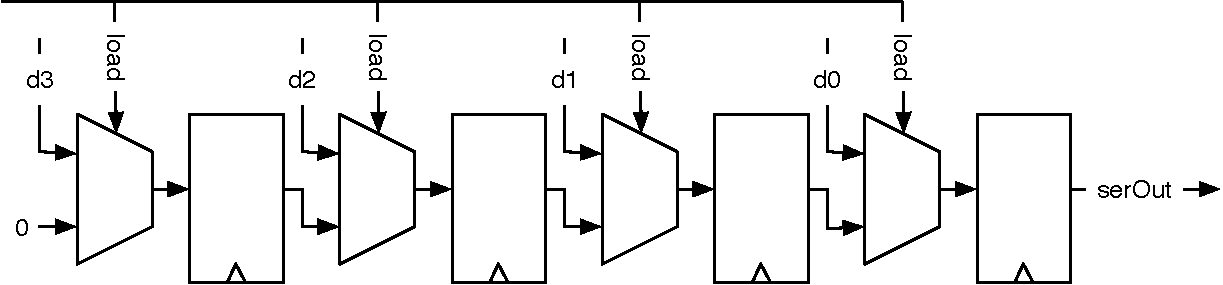
\includegraphics[scale=0.6]{figures/shiftreg-paraload}
  \caption{Thanh ghi dịch 4-bit với tải song song.}
  \label{fig:shiftreg-paraload}
\end{figure}

Hình~\ref{fig:shiftreg-paraload} biểu diễn thanh ghi dịch 4-bit với chức năng tải song song.
Mô tả Chisel của chức năng đó tương đối dễ hiểu như sau:

\shortlist{code/shift_paraload.txt}

Lưu ý rằng bây giờ chúng đang dịch sang bên phải, nên điền vào các số 0 ở MSB. 

\section{Bộ nhớ}
\index{Bộ nhớ}
\index{RAM}
\index{SRAM}

Một bộ nhớ có thể được tạo ra từ một tập hợp các thanh ghi, trong Chisel, một \code{Reg} của \code{Vec}.
Tuy nhiên, điều này là tốn kém về phần cứng và cấu trúc bộ nhớ lớn hơn được xây dựng dưới 
dạng \myref{https://en.wikipedia.org/wiki/Static_random-access_memory}{SRAM}.
Đối với ASIC, một trình biên dịch bộ nhớ dùng để xây dựng các bộ nhớ.
FPGA chứa các khối bộ nhớ trên chip, còn được gọi là các RAM khối.
Các khối bộ nhớ trên chip đó có thể được kết hợp để tạo ra các bộ nhớ lớn hơn.
Các bộ nhớ trong FPGA thường có một cổng đọc và một cổng ghi hoặc hai cổng có thể 
được chuyển đổi giữa đọc và ghi trong thời gian chạy. 

\index{Bộ nhớ đồng bộ}
FPGA (và cả ASIC) thường hỗ trợ bộ nhớ đồng bộ.
Bộ nhớ đồng bộ có các thanh ghi ở ngõ vào (địa chỉ đọc và ghi, dữ liệu ghi và cho phép ghi). 
Điều đó có nghĩa là dữ liệu đọc có sẵn trong một chu kỳ xung clock sau khi thiết lập địa chỉ. 

\begin{figure}
  \centering
  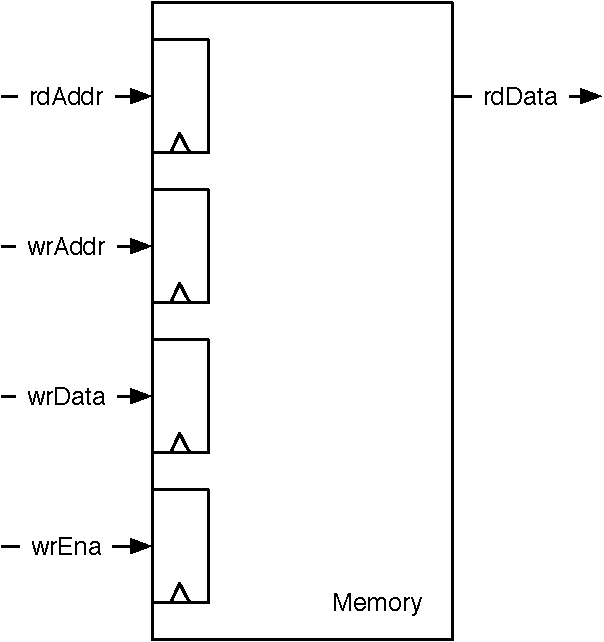
\includegraphics[scale=\scale]{figures/memory}
  \caption{Bộ nhớ đồng bộ.}
  \label{fig:memory}
\end{figure}

Hình~\ref{fig:memory} biểu diễn sơ đồ mạch của một bộ nhớ đồng bộ.
Bộ nhớ có hai cổng với một cổng đọc và một cổng ghi dữ liệu.
Cổng đọc có một ngõ vào duy nhất, địa chỉ đọc (\code{rdAddr}) và
một ngõ ra, dữ liệu đọc (\code{rdData}).
Cổng ghi có ba ngõ vào: địa chỉ (\code{wrAddr}), dữ liệu 
được ghi (\code{wrData}), và chân cho phép ghi (\code{wrEna}).
Lưu ý rằng đối với tất cả các ngõ vào, có một thanh ghi trong bộ nhớ hiển thị hành vi đồng bộ.


Để hỗ trợ bộ nhớ trên chip, Chisel cung cấp hàm tạo bộ nhớ \code{SyncReadMem}.
Listing~\ref{lst:memory} biểu diễn một thành phần \code{bộ nhớ} thực thi
1~KiB bộ nhớ với dữ liệu ngõ vào và ngõ ra có độ rộng 1 byte (8-bit) và một chân cho phép ghi.

\longlist{code/memory.txt}{1\,KiB bộ nhớ đồng bộ.}{lst:memory}

Một câu hỏi thú vị là giá trị nào được trả về từ một lần đọc khi trong cùng một 
chu kỳ xung clock, một giá trị mới được ghi vào ở cùng địa chỉ được đọc ra.
Chúng ta quan tâm đến hành vi đọc-trong-quá-trình-ghi của bộ nhớ.
Có ba khả năng: giá trị được ghi mới, giá trị cũ hoặc không xác định 
(có thể là sự kết hợp của một số bit từ giá trị cũ và một số dữ liệu được ghi mới).
Khả năng nào khả dụng trong FPGA phụ thuộc vào loại FPGA và đôi khi có thể được xác định.
Ở các tài liệu Chisel, dữ liệu đọc là không xác định. 

\begin{figure}
  \centering
  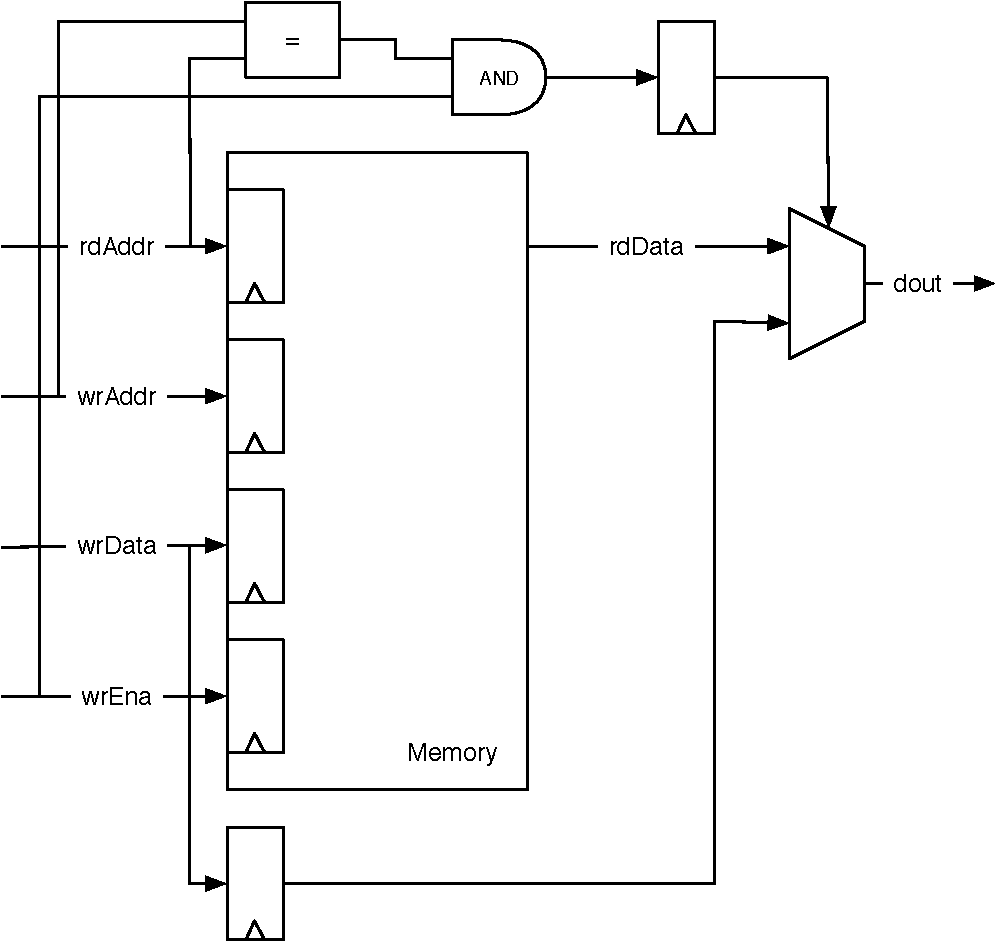
\includegraphics[scale=\scale]{figures/memory-forwarding}
  \caption{Bộ nhớ đồng bộ với chuyển tiếp cho một hành vi đọc-trong-quá-trình-ghi đã được định nghĩa.}
  \label{fig:memory:forwarding}
\end{figure}

\index{Chuyển tiếp dữ liệu}
Nếu muốn đọc ra giá trị được ghi mới, chúng ta có thể xây dựng một mạch điện 
chuyển tiếp để phát hiện rằng các địa chỉ bằng nhau và \emph{chuyển tiếp} dữ liệu ghi. 
Hình~\ref{fig:memory:forwarding} biểu diễn bộ nhớ với mạch chuyển tiếp. 
Địa chỉ đọc và ghi được so sánh và kiểm soát với chân cho phép ghi để chọn giữa 
đường chuyển tiếp của dữ liệu ghi hoặc dữ liệu đọc trong bộ nhớ. 
Dữ liệu ghi bị trễ một chu kỳ xung clock với một thanh ghi. 

Listing~\ref{lst:memory:forward} biểu diễn mã Chisel cho bộ nhớ đồng bộ
bao gồm mạch điện chuyển tiếp. Chúng ta cần lưu trữ dữ liệu ghi vào một thanh ghi
(\code{wrDataReg}) khả dụng trong chu kỳ xung clock tiếp theo để phù hợp với
bộ nhớ đồng bộ, thanh ghi đó cũng sẽ cung cấp giá trị đọc trong chu kỳ xung clock tiếp theo.
Chúng ta so sánh hai địa chỉ ngõ vào (\code{wrAddr} và \code{rdAddr})
và kiểm tra \code{wrEna} là đúng với điều kiện chuyển tiếp hay không.
Điều kiện này cũng bị trễ một chu kỳ xung clock.
Mạch đa hợp sẽ lựa chọn giữa dữ liệu (ghi) chuyển tiếp hoặc dữ liệu đọc từ bộ nhớ. 

\longlist{code/memory_forwarding.txt}{Bộ nhớ với mạch chuyển tiếp.}{lst:memory:forward}

Chisel còn cung cấp \code{Mem} để biểu diễn bộ nhớ với hoạt động ghi đồng bộ và đọc bất đồng bộ. 
Vì loại bộ nhớ này thường không khả dụng trực tiếp trong FPGA, nên công cụ tổng hợp sẽ xây dựng nó 
mà không dùng các flip-flop. Do đó, lời khuyên là các bạn nên sử dụng \code{SyncReadMem}. 

\section{Bài tập}

Sử dụng mạch mã hóa LED 7-đoạn từ bài tập trước và thêm mạch đếm 4-bit làm ngõ vào 
để hiển thị lần lượt từ \code{0} đến \code{F}. Khi kết nối trực tiếp mạch đếm 
này với tín hiệu xung clock của bo mạch FPGA, các bạn sẽ thấy tất cả 16 số chồng 
lên nhau (tất cả 7 đoạn sẽ sáng lên). Do đó, bạn cần phải làm chậm mạch đếm lại. 
Tạo một mạch đếm khác có thể tạo ra một tín hiệu \emph{tick} chu kỳ đơn có chu kỳ mỗi 500 mili-giây.
Sử dụng tín hiệu đó làm tín hiệu điều khiển cho mạch đếm 4-bit. 

Xây dựng dạng sóng PWM với hàm sinh tạo và đặt giá trị ngưỡng với hàm (hàm tam giác hoặc hàm sin).
Một hàm tam giác có thể được tạo ra bằng cách đếm lên và đếm xuống. Một hàm sin với 
việc sử dụng bảng tra mà các bạn có thể tạo ra với vài dòng mã Scala (xem Phần~\ref{sec:gen:comb:logic}).
Điều khiển đèn LED trên bo mạch FPGA với hàm PWM đã được điều biến đó. 
Tín hiệu PWM của các bạn sẽ là tần số nào? Bộ điều khiển đang chạy với tần số nào? 

Các thiết kế mạch số thường được phác thảo dưới dạng một mạch điện trên giấy. Không phải tất cả các chi tiết cần phải được hiển thị.
Chúng ta sử dụng sơ đồ khối, giống như trong các hình trong cuốn sách này. Đó là một kỹ năng quan trọng để có thể dịch trôi chảy giữa biểu diễn sơ đồ bản vẽ mạch điện và mô tả Chisel.
Vẽ sơ đồ khối cho các mạch sau: 

\shortlist{code/draw_mux6.txt}

\noindent Đây là một mạch phức tạp hơn một chút, chứa một thanh ghi:

\shortlist{code/draw_acc.txt}

\todo{Luca: More exercises would be nice. Maybe in the future?}

\chapter{Xử lý ngõ vào}

Các tín hiệu ngõ vào từ thế giới bên ngoài vào mạch đồng bộ thường không đồng bộ với xung clock; chúng bất đồng bộ. Một tín hiệu ngõ vào có thể đến từ một nguồn không có quá trình chuyển tiếp rõ ràng từ 0 sang 1 hoặc 1 sang 0. Một ví dụ là nút bật hoặc công tắc gạt. Tín hiệu ngõ vào có thể bị nhiễu với các xung nhọn có thể kích hoạt quá trình chuyển tiếp trong mạch đồng bộ. Chương này mô tả các mạch điện xử lý các điều kiện ngõ vào như vậy.

Hai vấn đề sau, công tắc chống dội và lọc nhiễu, cũng có thể được giải quyết bởi các thành phần tương tự, bên ngoài. Tuy nhiên, sẽ hiệu quả hơn (chi phí) để xử lý những vấn đề đó trong miền kỹ thuật số. 

\section{Ngõ vào bất đồng bộ}
\index{Ngõ vào bất đồng bộ}
\index{Trạng thái bất ổn định}


\todo{read Dally on this topic to check for correct wording and facts.}

Tín hiệu ngõ vào không đồng bộ với xung clock hệ thống được gọi là tín hiệu bất đồng bộ. Những tín hiệu đó có thể vi phạm thời gian thiết lập (setup time) và lưu giữ (hold time) của ngõ vào flip-flop. Vi phạm này có thể dẫn đến \myref{https://en.wikipedia.org/wiki/Metastability_(electronics)}{sự bất ổn định (Metastability)} của flip-flop. Sự bất ổn định có thể dẫn đến giá trị ngõ ra từ 0 đến 1 hoặc nó có thể tạo ra dao động. Tuy nhiên, sau một thời gian, flip-flop sẽ ổn định ở mức 0 hoặc 1.

Chúng ta không thể tránh được sự bất ổn định, nhưng chúng ta có thể ngăn chặn những ảnh hưởng của nó. Một giải pháp cổ điển là sử dụng hai flip-flop ở ngõ vào. Giả định là: khi flip-flop đầu tiên trở nên bất ổn định, nó sẽ phân giải thành trạng thái ổn định trong chu kỳ xung clock để thời gian thiết lập và thời gian lưu giữ của flip-flop thứ hai sẽ không bị vi phạm. 


\begin{figure}
  \centering
  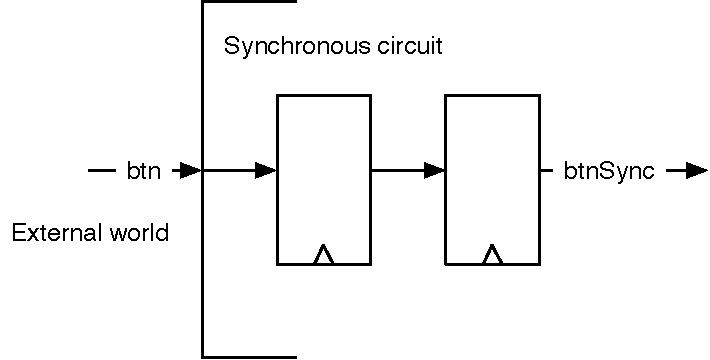
\includegraphics[scale=\scale]{figures/synchronizer}
  \caption{Mạch đồng bộ ngõ vào.}
  \label{fig:synchronizer}
\end{figure}

Hình~\ref{fig:synchronizer} thể hiện ranh giới giữa mạch đồng bộ và thế giới bên ngoài. Mạch đồng bộ hóa ngõ vào bao gồm hai flip-flop. Mã Chisel cho mạch đồng bộ ngõ vào là một dòng duy nhất tạo ra hai thanh ghi.

\shortlist{code/input_sync.txt}

Tất cả các tín hiệu bên ngoài bất đồng bộ cần một bộ đồng bộ ngõ vào.\footnote{Trường hợp ngoại lệ là khi tín hiệu ngõ vào phụ thuộc vào tín hiệu ngõ ra đồng bộ và chúng ta biết độ trễ đường truyền cực đại. Một ví dụ cổ điển là giao tiếp một SRAM bất đồng bộ với một mạch đồng bộ, ví dụ: bởi bộ vi xử lý.} Chúng ta cũng cần đồng bộ hóa một tín hiệu reset bên ngoài. Tín hiệu reset phải đi qua hai flip-flop trước khi nó được sử dụng làm tín hiệu reset cho các flip-flop khác trong mạch. Việc hủy xác nhận của tín hiệu reset cần đồng bộ với xung clock. 

\section{Chống dội}
\index{Chống dội}

Các công tắc và nút nhấn có thể cần một khoảng thời gian để chuyển đổi giữa bật và tắt. Trong quá trình chuyển đổi, công tắc có thể bị dội giữa hai trạng thái đó. Nếu chúng ta sử dụng một tín hiệu như vậy mà không xử lý thêm, chúng ta có thể phát hiện nhiều sự kiện chuyển tiếp hơn chúng ta mong muốn. Một giải pháp là sử dụng thời gian để lọc bỏ sự dội này. Giả sử thời gian dội tối đa là $t_{bounce}$, chúng ta sẽ lấy mẫu tín hiệu đầu vào với khoảng thời gian $T>t_{bounce}$. Chúng ta sẽ chỉ sử dụng tín hiệu được lấy mẫu thêm ở luồng xuống.

Khi lấy mẫu ngõ vào với khoảng thời gian dài này, chúng ta biết rằng, khi chuyển từ 0 sang 1, chỉ một mẫu có thể rơi vào vùng dội. Mẫu trước đó sẽ đọc an toàn 0 và mẫu sau vùng dội sẽ đọc an toàn 1. Mẫu trong vùng dội sẽ là 0 hoặc 1. Tuy nhiên, điều này không quan trọng vì sau đó nó thuộc về hoặc vẫn là các mẫu 0 hoặc các mẫu 1 có sẵn. Điểm mấu chốt là chúng ta chỉ có một lần chuyển đổi từ 0 sang 1. 

\begin{figure}
  \centering
  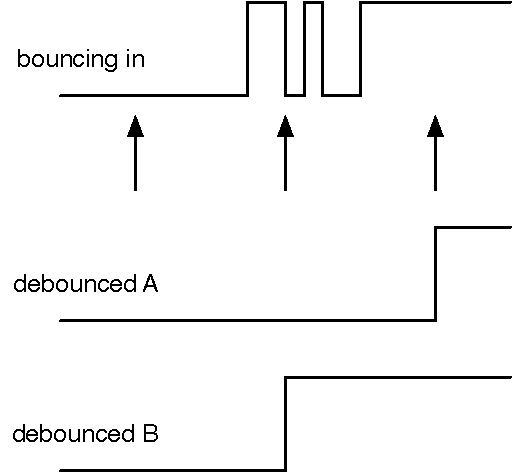
\includegraphics[scale=\scale]{figures/debounce}
  \caption{Chống dội tín hiệu ngõ vào.}
  \label{fig:debounce}
\end{figure}

Hình ~\ref{fig:debounce} biểu diễn quá trình hoạt động lấy mẫu để chống dội. Tín hiệu trên cùng biểu diễn ngõ vào bị dội và các mũi tên bên dưới biểu diễn các điểm lấy mẫu. Khoảng cách giữa các điểm lấy mẫu đó cần phải dài hơn thời gian dội tối đa. Mẫu đầu tiên lấy mẫu an toàn 0, và mẫu sau trong hình lấy mẫu 1. Mẫu giữa rơi vào thời gian dội. Nó có thể là 0 hoặc 1. Hai kết quả có thể xảy ra được hiển thị là \code{debounce A} và \code{debounce B}. Cả hai đều có một lần chuyển đổi duy nhất từ 0 sang 1. Sự khác biệt duy nhất giữa hai kết quả này là quá trình chuyển đổi trong phiên bản B muộn hơn một chu kỳ mẫu. Tuy nhiên, đây thường không phải là vấn đề.

Mã Chisel cho việc chống dội được phát triển hơn một chút so với mã cho mạch đồng bộ. Chúng ta tạo ra thời gian mẫu bằng một mạch đếm cung cấp một tín hiệu chu kỳ đơn \code{tick}, như chúng ta đã thực hiện trong Phần ~\ref{sec:gen:timing}. 

\shortlist{code/input_fac.txt}
\shortlist{code/input_debounce.txt}

Đầu tiên, chúng ta cần quyết định tần số lấy mẫu. Ví dụ trên giả định xung clock 100~MHz và suy ra tần số lấy mẫu là 100~Hz (giả sử rằng thời gian dội là dưới 10~ms). Giá trị mạch đếm cực đại là \code{FAC}, hệ số chia. Chúng ta định nghĩa thanh ghi \code{btnDebReg} cho tín hiệu chống dội, không có giá trị reset. Thanh ghi \code{cntReg} đóng vai trò là mạch đếm, và tín hiệu \code{tick} là đúng khi mạch đếm đạt đến giá trị lớn nhất. Trong trường hợp đó, điều kiện \code{when} là \code{true} và (1) mạch đếm được reset về 0 và (2) thanh ghi chống dội lưu trữ mẫu ngõ vào. Trong ví dụ, tín hiệu ngõ vào được đặt tên là \code{btnSync} vì nó là ngõ ra từ mạch đồng bộ ngõ vào đã được trình bày trong phần trước.

Mạch chống dội đi sau mạch đồng bộ. Đầu tiên, chúng ta cần đồng bộ hóa trong tín hiệu bất đồng bộ, sau đó chúng ta có thể xử lý thêm nó trong miền kỹ thuật số. 

\section{Lọc tín hiệu ngõ vào}

\index{Biểu quyết đa số}

Đôi khi tín hiệu ngõ vào có thể bị nhiễu, có thể nó chứa các xung nhọn mà chúng ta có thể lấy mẫu không chủ ý với mạch đồng bộ ngõ vào và bộ chống dội. Một tùy chọn để lọc các xung đột biến ngõ vào đó là sử dụng mạch biểu quyết đa số. Trong trường hợp đơn giản nhất, chúng ta lấy ba mẫu và thực hiện biểu quyết đa số. \myref{https://en.wikipedia.org/wiki/Majority_function}{Hàm đa số}, có liên quan đến hàm trung vị, cho ra giá trị của đa số. Trong trường hợp này, khi chúng ta sử dụng lấy mẫu để chống dội, chúng ta thực hiện biểu quyết đa số đối với tín hiệu được lấy mẫu. Biểu quyết đa số đảm bảo rằng tín hiệu ổn định lâu hơn chu kỳ lấy mẫu. 

\begin{figure}
  \centering
  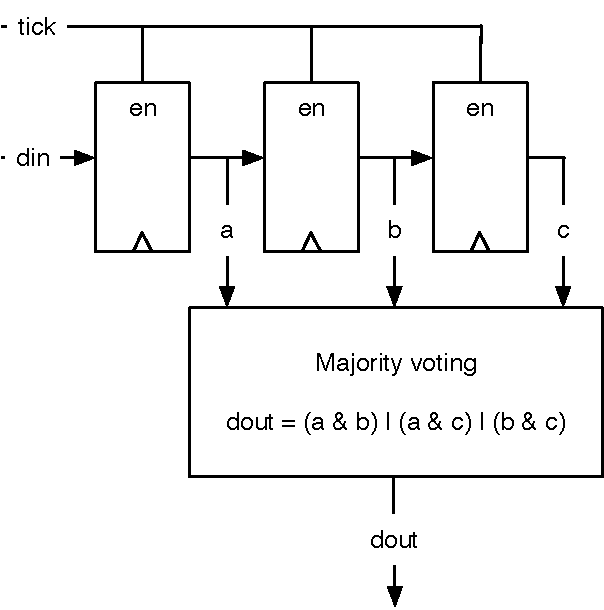
\includegraphics[scale=\scale]{figures/majority}
  \caption{Biểu quyết đa số trên tín hiệu ngõ vào lấy mẫu.}
  \label{fig:majority}
\end{figure}

Hình~\ref{fig:majority} biểu diễn mạch biểu quyết đa số. Nó bao gồm một thanh ghi dịch 3-bit được điều khiển bởi tín hiệu \code{tick} mà chúng ta đã sử dụng để lấy mẫu chống dội. Ngõ ra của ba thanh ghi được đưa vào mạch biểu quyết đa số. Chức năng biểu quyết đa số lọc bất kỳ sự thay đổi tín hiệu nào ngắn hơn chu kỳ lấy mẫu.

Mã Chisel sau đây trình bày thanh ghi dịch 3-bit, được điều khiển bởi tín hiệu \code{tick} và hàm biểu quyết, kết quả ở tín hiệu \code{btnClean}.

Lưu ý rằng rất ít khi cần đến biểu quyết đa số. 

\shortlist{code/input_majority.txt}

Để sử dụng đầu ra của tín hiệu đầu vào đã được xử lý cẩn thận, trước tiên chúng ta dò cạnh lên bởi thành phần trì hoãn \code{RegNext} và sau đó so sánh tín hiệu này với giá trị hiện tại của \code{btnClean} để điều khiển mạch đếm tăng lên. 

\index{Dò cạnh}

\shortlist{code/input_usage.txt}

\section{Kết hợp xử lý ngõ vào với các hàm}

Để tóm tắt phần xử lý đầu vào, chúng ta biểu diễn thêm một số mã Chisel. Vì các mạch điện đã được trình bày có thể là nhỏ, nhưng là các khối xây dựng có thể tái sử dụng, chúng ta gói gọn chúng trong các hàm. Phần ~\ref{sec:functions} đã chỉ ra cách chúng ta có thể trừu tượng hóa các khối xây dựng nhỏ trong các hàm Chisel nhẹ thay vì dùng các mô-đun đầy đủ. Các hàm Chisel đó tạo ra các thực thể phần cứng, ví dụ: hàm \code{sync} tạo hai flip-flop kết nối với ngõ vào và kết nối với nhau. Hàm trả về ngõ ra của flip-flop thứ hai. Nếu hữu ích, các hàm đó có thể được nâng lên thành một số đối tượng lớp tiện ích. 

\longlist{code/input_func.txt}{Tóm tắt xử lý ngõ vào với các hàm.}{lst:input:func}

\section{Bài tập}

Xây dựng một mạch đếm được đếm lên bởi một nút nhấn ở ngõ vào. Hiển thị giá trị của mạch đếm ở dạng nhị phân trên các đèn LED của bo mạch FPGA. Xây dựng chuỗi xử lý đầu vào hoàn chỉnh với: (1) mạch đồng bộ hóa ngõ vào, (2) mạch chống dội, (3) mạch biểu quyết đa số để khử nhiễu, và (4) mạch dò cạnh để kích hoạt tăng mạch đếm.

Vì không có gì đảm bảo rằng nút nhấn hiện đại sẽ luôn bị dội, các bạn có thể mô phỏng độ dội và xung nhọn bằng cách nhấn nút theo cách thủ công liên tiếp nhanh và sử dụng tần số lấy mẫu thấp. Chọn, ví dụ: một giây làm tần số mẫu, tức là nếu xung clock ngõ vào hoạt động ở 100~MHz, thì hãy chia nó cho 100.000.000. Mô phỏng một nút dội bằng cách nhấn nhiều lần liên tiếp trước khi chuyển sang nhấn ổn định. Kiểm tra mạch của các bạn khi không có và khi có mạch chống dội lấy mẫu ở 1~Hz. Với biểu quyết đa số, các bạn cần nhấn từ một đến hai giây để đảm bảo mạch đếm tăng lên. Ngoài ra, việc nhả nút nhấn được tính là biểu quyết đa số. Do đó, mạch chỉ nhận ra việc nhả nút khi nó dài hơn 1-2 giây. 

\chapter{Máy trạng thái hữu hạn}
\index{Máy trạng thái hữu hạn}
\index{FSM}
\index{Mạch tuần tự đồng bộ}

Máy trạng thái hữu hạn (Finite-State Machine - FSM) là một khối xây dựng cơ bản trong thiết kế mạch số. FSM có thể được mô tả như một tập hợp \emph{các trạng thái} và các \emph{chuyển tiếp trạng thái} có điều kiện (được bảo vệ) giữa các trạng thái. Một FSM có trạng thái ban đầu, trạng thái này được đặt khi reset. FSM còn được gọi là mạch tuần tự đồng bộ.

Việc triển khai FSM bao gồm ba phần: (1) thanh ghi lưu giữ trạng thái hiện tại, (2) mạch logic tổ hợp tính toán trạng thái kế tiếp phụ thuộc vào trạng thái hiện tại và ngõ vào, và (3) mạch logic tổ hợp tính toán ngõ ra của FSM.

Về nguyên tắc, mọi mạch số có chứa một thanh ghi hoặc các phần tử bộ nhớ khác để lưu trữ trạng thái đều có thể được mô tả như một FSM đơn lẻ. Tuy nhiên, điều này có thể không thực tế, ví dụ: hãy thử mô tả máy tính xách tay của các bạn như một FSM đơn lẻ. Trong chương tiếp theo, chúng ta sẽ mô tả cách xây dựng các hệ thống lớn hơn từ các FSM nhỏ hơn bằng cách kết hợp chúng thành các FSM giao tiếp. 

\section{Máy trạng thái hữu hạn cơ bản}

\begin{figure}
  \centering
  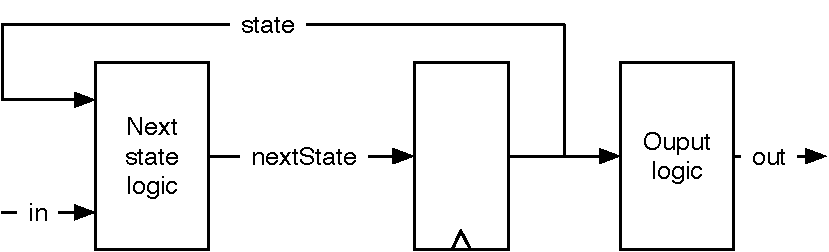
\includegraphics[scale=\scale]{figures/fsm}
  \caption{Máy trạng thái hữu hạn (kiểu Moore).}
  \label{fig:fsm}
\end{figure}

Hình ~\ref{fig:fsm} biểu diễn sơ đồ mạch điện của một FSM. Thanh ghi chứa \code{trạng thái} hiện tại.
Mạch logic trạng thái kế tiếp sẽ tính toán giá trị của trạng thái kế tiếp (\code{next\_state}) từ trạng thái hiện tại \code{state} và ngõ vào (\code{in}).
Ở chu kỳ xung clock tiếp theo, \code{state} trở thành \code{next\_state}.
Mạch logic ngõ ra tính toán ngõ ra (\code{out}). Vì ngõ ra chỉ phụ thuộc vào trạng thái hiện tại nên máy trạng thái này được gọi là
\myref{https://en.wikipedia.org/wiki/Moore_machine}{Máy trạng thái kiểu Moore}.
\index{Máy trạng thái hữu hạn!Moore}


\myref{https://en.wikipedia.org/wiki/State_diagram}{Lưu đồ trạng thái} mô tả hoạt động của FSM một cách trực quan.
Trong lưu đồ trạng thái, các trạng thái riêng lẻ được mô tả dưới dạng các vòng tròn được gắn nhãn với tên trạng thái. Các chuyển đổi trạng thái được biểu diễn bằng các mũi tên giữa các trạng thái. Bảo vệ (hoặc điều kiện), khi chuyển đổi này được thực hiện, được vẽ như một nhãn cho mũi tên. 

\index{Lưu đồ trạng thái}

Hình~\ref{fig:diag-moore} biểu diển lưu đồ trạng thái của một ví dụ FSM đơn giản.
FSM có ba trạng thái: \emph{green}, \emph{orange}, and \emph{red},
chỉ thị mức độ báo động. FSM bắt đầu ở mức \emph{green}.
Khi có một \emph{sự kiện xấu} xảy ra mức báo động được chuyển sang \emph{orange}.
Trong sự kiện xấu thứ hai, mức báo động được chuyển sang \emph{red}.
Trong trường hợp đó, chuông sẽ reo; \emph{ring bell} là ngõ ra duy nhất của FSM này.
Chúng ta thêm ngõ ra vào trạng thái \emph{red}.
Báo động có thể được reset bởi tín hiệu \emph{clear}.

\begin{figure}
  \centering
  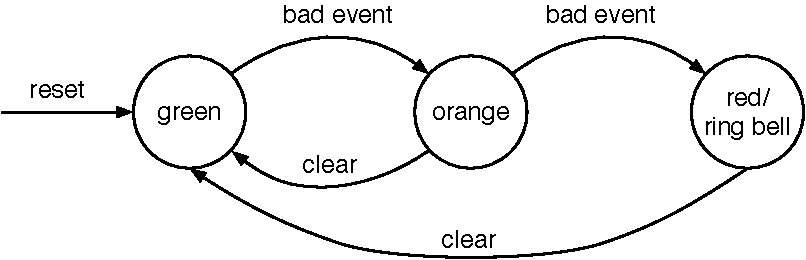
\includegraphics[scale=\scale]{figures/state-diag-moore}
  \caption{Lưu đồ trạng thái của một FSM báo động.}
  \label{fig:diag-moore}
\end{figure}

Mặc dù một lưu đồ trạng thái trực quan và chức năng của FSM có thể được nắm bắt nhanh chóng, nhưng một bảng trạng thái có thể được ghi xuống nhanh hơn. Bảng ~\ref{tab:state:table} hiển thị bảng trạng thái cho FSM báo động. Chúng ta liệt kê trạng thái hiện tại, các giá trị ngõ vào, kết quả trạng thái kế tiếp và giá trị ngõ ra cho trạng thái hiện tại. Về nguyên tắc, chúng ta sẽ cần xác định tất cả các ngõ vào có thể có cho tất cả các trạng thái có thể. Bảng này sẽ có $3 \times 4 = 12$ hàng. Chúng ta đơn giản hóa bảng bằng cách chỉ ra rằng ngõ vào \emph{clear} là tín hiệu don't care (không quan tâm) khi \emph{sự kiện xấu} xảy ra. Điều đó có nghĩa là \emph{sự kiện xấu} được ưu tiên hơn tín hiệu \emph{clear}. Cột ngõ ra có một số lần lặp lại. Nếu chúng ta có FSM lớn hơn và/hoặc nhiều ngõ ra hơn, thì chúng ta có thể chia bảng thành hai, một cho logic trạng thái kế tiếp theo và một cho logic ngõ ra. 

\begin{table}
\centering
\caption{Bảng trạng thái của FSM báo động.}
\begin{tabular}{ccccc}
\toprule
& \multicolumn{2}{c}{Ngõ vào} \\
\cmidrule{2-3}
Trạng thái &  Sự kiện xấu & Xóa & Trạng thái kế tiếp & Chuông reo \\
\midrule
green & 0 & 0 & green & 0 \\
green & 1 & - & orange & 0 \\
orange & 0 & 0 & orange & 0 \\
orange & 1 & - & red & 0 \\
orange & 0 & 1 & green & 0 \\
red & 0 & 0 & red & 1 \\
red & 0 & 1 & green & 1 \\
\bottomrule
\end{tabular}
\label{tab:state:table}
\end{table}

Cuối cùng, sau khi tất cả thiết kế của FSM mức báo động, chúng ta sẽ lập trình nó trong Chisel. Listing~\ref{lst:fsm:alarm} trình bày mã Chisel cho FSM báo động. Lưu ý kiểu \code{Bool} trong Chisel cho các ngõ vào và ngõ ra của FSM. Để dùng \code{Enum} và lệnh điều khiển \code{switch}, chúng ta cần nhập \code{chisel3.util.\_}.

\longlist{code/simple_fsm.txt}{Mã Chisel cho FSM báo động.}{lst:fsm:alarm}

Mã Chisel hoàn chỉnh cho FSM đơn giản này nằm gọn trong một trang.
Chúng ta hãy lướt qua các phần riêng lẻ.
FSM có hai tín hiệu ngõ vào và một tín hiệu ngõ ra, được ghi trong một \code{Bundle} Chisel:
%
\shortlist{code/simple_fsm_io.txt}

\noindent Khá nhiều công việc đã được dành để mã hóa trạng thái tối ưu. Hai tùy chọn phổ biến là mã hóa nhị phân hoặc mã hóa one-hot. Tuy nhiên, chúng ta để những quyết định mức-thấp đó cho công cụ tổng hợp và hướng tới mã code có thể đọc được.\footnote{Trong phiên bản hiện tại của Chisel, kiểu \code{Enum} biểu diễn các trạng thái trong mã hóa nhị phân. Nếu chúng ta muốn một dạng mã hóa khác, ví dụ: mã hóa one-hot, chúng ta có thể định nghĩa hằng số Chisel cho tên trạng thái.} Do đó, chúng ta sử dụng kiểu liệt kê với tên tượng trưng cho các trạng thái: 

\shortlist{code/simple_fsm_states.txt}

\noindent Các giá trị trạng thái riêng lẻ như trong danh sách, trong đó các phần tử riêng lẻ được ghép nối bởi toán tử \code{::}; \code{Nil} biểu diễn phần kết thúc của danh sách. Một thực thể \code{Enum} được \emph{gán} cho danh sách các trạng thái.
Thanh ghi giữ trạng thái được định nghĩa với trạng thái \emph{green} như giá trị reset:

\shortlist{code/simple_fsm_register.txt}

\noindent Phần quan trọng của FSM là ở logic trạng thái tiếp theo. Chúng ta sử dụng công tắc Chisel trên thanh ghi trạng thái để bao gồm tất cả các trạng thái. Trong mỗi trạng thái \code{là} nhánh mà chúng ta sẽ lập trình cho logic trạng thái tiếp theo, tùy thuộc vào các ngõ vào, bằng cách gán một giá trị mới cho thanh ghi trạng thái: 

\shortlist{code/simple_fsm_next.txt}

\noindent Cuối cùng, nhưng không phải sau cùng, chúng ta lập trình ngõ ra \emph{ring bell} là giá trị đúng (true) khi trạng thái là \emph{red}.

\shortlist{code/simple_fsm_output.txt}

Lưu ý rằng chúng ta đã \emph{không} đưa vào tín hiệu \code{next\_state} cho ngõ vào thanh ghi, vì đây là bài thực hành phổ biến trong Verilog hoặc VHDL. Các thanh ghi trong Verilog và VHDL được mô tả theo một cú pháp đặc biệt và không thể được gán (và không được gán lại) trong một khối mạch tổ hợp. Do đó, tín hiệu bổ sung, được tính toán trong một khối mạch tổ hợp, được đưa vào và kết nối với ngõ vào thanh ghi. Trong Chisel, một thanh ghi là một kiểu cơ sở và có thể được sử dụng tự do trong một khối mạch tổ hợp. 

\section{Ngõ ra nhanh hơn với FSM Mealy}

Với FSM Moore, ngõ ra chỉ phụ thuộc vào trạng thái hiện tại. Điều đó có nghĩa là sự thay đổi của ngõ vào có thể được xem như là thay đổi của ngõ ra \emph{sớm nhất} trong chu kỳ xung clock tiếp theo. Nếu chúng ta muốn quan sát sự thay đổi tức thời, chúng ta cần một đường dẫn tổ hợp từ ngõ vào đến ngõ ra. Chúng ta hãy cùng xem xét một ví dụ tối thiểu, một mạch dò cạnh. Chúng ta đã thấy lệnh Chisel theo kiểu một dòng duy nhất này trước đây:

\shortlist{code/sequ_reg_rising.txt}

\begin{figure}
  \centering
  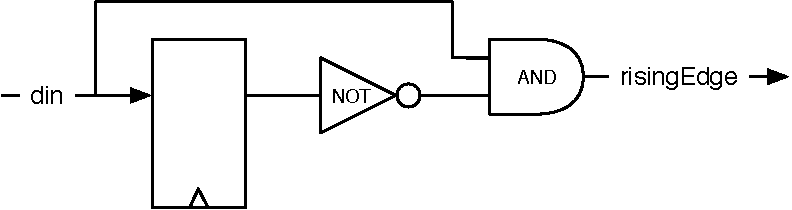
\includegraphics[scale=\scale]{figures/fsm-rising}
  \caption{Mạch dò cạnh lên (FSM kiểu Mealy).}
  \label{fig:fsm-rising}
\end{figure}

Hình ~\ref{fig:fsm-rising} biểu diễn sơ đồ mạch điện của mạch dò cạnh lên. Ngõ ra trở thành 1 trong một chu kỳ xung clock khi giá trị ngõ vào hiện tại là 1 và ngõ vào trong chu kỳ xung clock cuối cùng là 0. Thanh ghi trạng thái chỉ là một flip-flop D duy nhất trong đó trạng thái tiếp theo chỉ là ngõ vào. Chúng ta cũng có thể coi đây là phần tử trễ của một chu kỳ xong clock. Logic ngõ ra \emph{so sánh} ngõ vào hiện tại với trạng thái hiện tại. 

Khi ngõ ra cũng phụ thuộc vào ngõ vào, tức là, có một đường tổ hợp giữa ngõ vào của FSM và ngõ ra, điều này được gọi là 
\myref{https://en.wikipedia.org/wiki/Mealy_machine}{máy Mealy}.
\index{Máy trạng thái hữu hạn!Mealy}

\begin{figure}
  \centering
  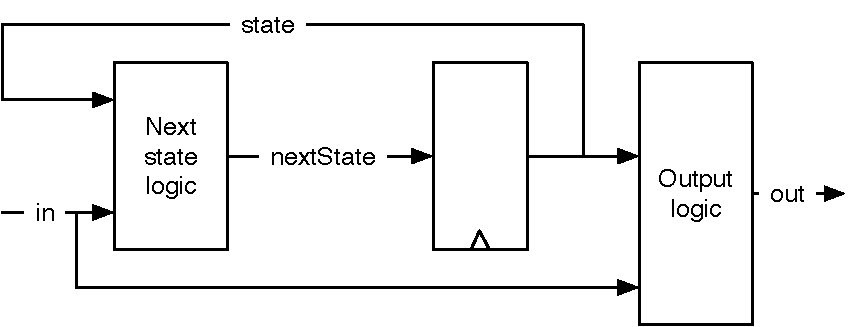
\includegraphics[scale=\scale]{figures/mealy}
  \caption{Máy trạng thái hữu hạn kiểu Mealy.}
  \label{fig:mealy}
\end{figure}

Hình ~\ref{fig:mealy} biểu diễn sơ đồ mạch của FSM kiểu Mealy. Tương tự như FSM kiểu Moore, thanh ghi chứa \code {trạng thái} hiện tại và logic trạng thái tiếp theo tính toán giá trị trạng thái tiếp theo (\code{next\_state}) từ \code{trạng thái} hiện tại và ngõ vào (\code{in}). Vào chu  kỳ xung clock tiếp theo, \code{state} trở thành \code{next\_state}. Logic ngõ ra tính toán ngõ ra (\code{out}) từ trạng thái hiện tại \emph{và} ngõ vào cho FSM. 

\begin{figure}
  \centering
  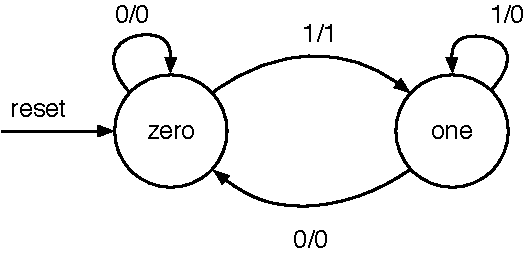
\includegraphics[scale=\scale]{figures/state-diag-mealy}
  \caption{Lưu đồ trạng thái của mạch dò cạnh lên trong FSM kiểu Mealy.}
  \label{fig:diag:mealy}
\end{figure}

Hình ~\ref{fig:diag:mealy} biểu diễn lưu đồ trạng thái của FSM Mealy cho mạch dò cạnh. Vì thanh ghi trạng thái chỉ bao gồm một flip-flop D duy nhất, nên chỉ có thể có hai trạng thái đặt tên là \code{zero} và \code{one} trong ví dụ này. Vì ngõ ra của FSM Mealy không chỉ phụ thuộc vào trạng thái mà còn phụ thuộc vào ngõ vào, nên chúng ta không thể mô tả ngõ ra như một phần của vòng tròn trạng thái. Thay vào đó, các chuyển đổi giữa các trạng thái được gắn nhãn với giá trị ngõ vào (điều kiện) \emph{và} ngõ ra (sau dấu gạch chéo). Cũng lưu ý rằng, chúng ta vẽ các trạng thái tự chuyển đổi, ví dụ: ở trạng thái \code{zero} khi ngõ vào là \code{0}, FSM vẫn ở trạng thái \code{zero} và ngõ ra là {0}. Ở cạnh lên, FSM chỉ tạo ra ngõ ra \code{1} khi chuyển đổi từ trạng thái \code{zero} sang trạng thái \code{one}. Trong trạng thái \code{one}, biểu diễn rằng ngõ vào bây giờ là \code{1}, ngõ ra là \code{0}. Chúng ta chỉ muốn một xung (chu kỳ) duy nhất cho mỗi cạnh lên của ngõ vào. 

\longlist{code/rising_fsm.txt}{Dò cạnh lên với FSM Mealy.}{lst:fsm:rising}

Listing~\ref{lst:fsm:rising} trình bày mã Chisel cho dò cạnh lên với máy Mealy.
Như ở ví dụ trước, chúng ta sử dụng kiểu \code{Bool} trong Chisel cho ngõ vào và ngõ ra đơn bit.
Logic ngõ ra bây giờ là một phần của logic trạng thái tiếp theo; trên chuyển tiếp từ
\code{zero} sang \code{one}, ngõ ra được đặt là \code{true.B}. Nếu không,
giá trị gán mặc định cho đếm ngõ ra là (\code{false.B}).

Người ta có thể hỏi liệu FSM toàn diện có phải là giải pháp tốt nhất cho mạch dò cạnh hay không, đặc biệt như chúng ta đã thấy cú pháp một dòng lệnh duy nhất trong Chisel cho cùng một chức năng. Việc tiêu thụ phần cứng cũng tương tự. Cả hai giải pháp đều cần một flip-flop D duy nhất cho trạng thái. Mạch logic tổ hợp cho FSM có lẽ phức tạp hơn một chút, do sự thay đổi trạng thái phụ thuộc vào trạng thái hiện tại và giá trị ngõ vào. Với chức năng này, điều quan trọng là kiểu viết một dòng lệnh duy nhất dễ viết và dễ đọc hơn. Do đó, kiểu viết một dòng lệnh duy nhất là giải pháp được ưa thích hơn.

Chúng ta đã sử dụng ví dụ này để biểu diễn một trong những FSM Mealy nhỏ nhất có thể. FSM sẽ được sử dụng cho các mạch điện phức tạp hơn với ba trạng thái trở lên. 

\section{So sánh Moore với Mealy}

Để chỉ ra sự khác biệt giữa FSM Moore và Mealy, chúng ta thực hiện lại việc dò cạnh bằng FSM Moore. 

\begin{figure}
  \centering
  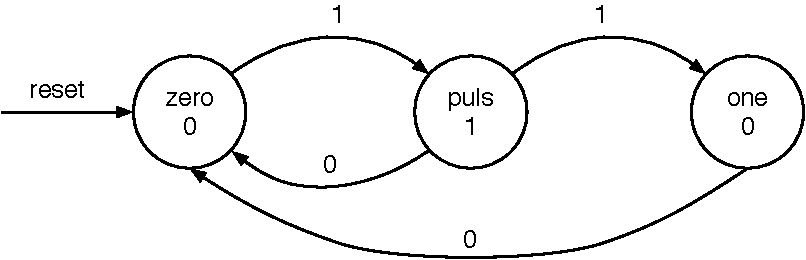
\includegraphics[scale=\scale]{figures/state-diag-rising-moore}
  \caption{Lưu đồ trạng thái mạch dò cạnh lên của FSM Moore.}
  \label{fig:diag:rising:moore}
\end{figure}

Hình ~\ref{fig:diag:rising:moore} biểu diễn lưu đồ trạng thái để dò cạnh lên với FSM Moore. Điều đầu tiên cần chú ý là FSM Moore cần ba trạng thái, so với hai trạng thái trong FSM Mealy. Trạng thái \code{puls} là cần thiết để tạo ra các xung chu kỳ đơn. FSM trong trạng thái \code{puls} chỉ cần một chu kỳ xung clock và sau đó tiếp tục trở lại trạng thái bắt đầu \code{zero} hoặc thành trạng thái \code{one}, chờ ngõ vào trở lại 0 lần nữa. Chúng ta biểu diễn điều kiện ngõ vào ở trên các mũi tên chuyển đổi trạng thái và ngõ ra FSM trong các vòng tròn biểu diễn trạng thái. 

\longlist{code/rising_moore_fsm.txt}{Dò cạnh lên với FSM Moore.}{lst:fsm:rising:moore}

Listing~\ref{lst:fsm:rising:moore} trình bày phiên bản Moore của mạch dò cạnh lên. Nó sử dụng gấp đôi số flip-flop D so với phiên bản Mealy hoặc được lập trình trực tiếp. Do đó, kết quả logic trạng thái tiếp theo cũng lớn hơn phiên bản Mealy hoặc được lập trình trực tiếp. 

\begin{figure}
  \centering
  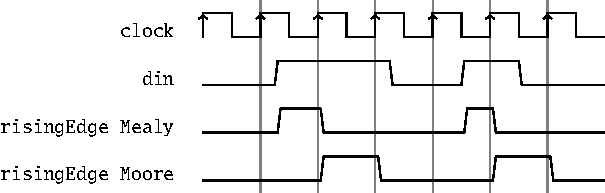
\includegraphics[scale=1]{figures/rising}
  \caption{Dạng sóng FSM Moore và Mealy cho dò cạnh lên.}
  \label{fig:rising}
\end{figure}

Hình ~\ref{fig:rising} biểu diễn dạng sóng của phiên bản Mealy và Moore của FSM dò cạnh lên. Chúng ta có thể thấy rằng ngõ ra Mealy theo sát cạnh lên ngõ vào, trong khi ngõ ra Moore tăng sau tick xung clock. Chúng ta cũng có thể thấy rằng ngõ ra Moore có độ rộng một chu kỳ xung clock, trong khi đó ngõ ra Mealy thường nhỏ hơn một chu kỳ xung clock.

Từ ví dụ trên, người ta muốn tìm FSM Mealy. FSM \emph{tốt hơn} vì chúng cần ít trạng thái hơn (và đó là logic) và đáp ứng nhanh hơn FSM Moore. Tuy nhiên, đường tổ hợp bên trong máy Mealy có thể gây ra rắc rối trong các thiết kế lớn hơn. Đầu tiên, với một chuỗi FSM giao tiếp (xem chương tiếp theo), đường tổ hợp này có thể trở nên dài. Thứ hai, nếu các FSM giao tiếp xây dựng một vòng tròn, kết quả là một vòng lặp tổ hợp, đây là một lỗi trong thiết kế đồng bộ. Do sự đứt đoạn trong đường tổ hợp với thanh ghi trạng thái trong FSM Moore, nên tất cả các vấn đề trên không tồn tại đối với FSM Moore giao tiếp.

Tóm lại, các FSM Moore kết hợp với nhau tốt hơn để giao tiếp các máy trạng thái; chúng \emph{mạnh mẽ hơn} so với FSM Mealy. Chỉ sử dụng các FSM Mealy khi yếu tố đáp ứng trong cùng một chu kỳ được xem là quan trọng nhất. Các mạch nhỏ như dò cạnh lên, thực tế là máy Mealy, cũng tốt. 

\section{Bài tập}

% This is a boring example, maybe I can find something more interesting
Trong chương này, các bạn đã thấy nhiều ví dụ về các FSM rất nhỏ. Bây giờ đã đến lúc viết một số mã FSM \emph{thực sự}. Chọn một ví dụ phức tạp hơn một chút, thực hiện FSM và viết testbench cho nó.

Một ví dụ cổ điển cho FSM là mạch điều khiển đèn giao thông (xem~\cite[Phần~14.3]{dally:vhdl:2016}). Mạch điều khiển đèn giao thông phải đảm bảo rằng quá trình chuyển đổi từ màu đỏ sang màu xanh lá cây có một pha ở giữa hai con đường trong giao lộ đều có đèn cấm đi (đỏ và cam). Để làm cho ví dụ này thú vị hơn một chút, hãy xem xét một đường ưu tiên. Đường phụ có hai mạch dò xe (trên cả hai lối vào giao lộ). Chỉ chuyển sang màu xanh cho đường phụ khi phát hiện có xe và sau đó chuyển về màu xanh cho đường ưu tiên. 

\todo{Luca: Greatest common divisor with Euclide algorithm can be also a nice exercise.
Martin: but this is shown at the Chisel homepage without an FSM.}

\todo{Here a more interesting exercise. And not one from Dally.}

\chapter{Máy trạng thái giao tiếp}
\index{Máy trạng thái giao tiếp}

Một vấn đề thường quá phức tạp để mô tả nó bằng một FSM duy nhất. Trong trường hợp đó, vấn đề có thể được chia thành hai hoặc nhiều FSM nhỏ hơn và đơn giản hơn. Các FSM đó sau đó giao tiếp với các tín hiệu. Một ngõ ra FSM này là một ngõ vào FSM khác và FSM theo dõi ngõ ra của FSM khác. Khi chúng ta chia một FSM lớn thành những FSM đơn giản hơn, điều này được gọi là các FSM phân số. Tuy nhiên, thường các FSM giao tiếp được thiết kế trực tiếp từ đặc tả kỹ thuật, vì thường một FSM đơn lẻ sẽ không khả thi. 

\section{Ví dụ mạch chớp đèn}

Để thảo luận các FSM giao tiếp, chúng ta sử dụng ví dụ từ ~\cite[Chương~17]{dally:vhdl:2016}, mạch chớp đèn.
Mạch chớp đèn có một ngõ vào \code{start} và một ngõ ra \code{light}. Đặc tả của mạch chớp đèn như sau:
\begin{itemize}
\item khi tín hiệu \code{start} lên cao trong một chu kỳ xung clock, quy trình chớp nháy bắt đầu;
\item quy trình nhấp nháy ba lần;
\item tín hiệu \code{light} sẽ \emph{bật} trong 6 chu kỳ xung clock, và \code{light} sẽ \emph{tắt} trong 4 chu kỳ xung clock giữa những lần chớp;
\item sau quy trình, FSM chuyển tín hiệu \code{light} \emph{tắt} và chờ đợi lần bắt đầu kế tiếp.
\end{itemize}

Thực hiện trực tiếp FSM\footnote{Lưu đồ trạng thái được biểu diễn trong ~\cite[p.~376]{dally:vhdl:2016}.} có 27 trạng thái:
trạng thái đầu tiên chờ giá trị ngõ vào, $3 \times 6$ trạng thái cho ba trạng thái \emph{on} và $2 \times 4$ trạng thái cho các trạng thái \emph{off}.
Mã code cho việc thực hiện mạch đèn chớp sáng đơn giản này không được trình bày. 

Vấn đề có thể được giải quyết một cách thanh thoát hơn bằng cách phân tách FSM lớn này thành hai FSM nhỏ hơn: FSM chủ (Master FSM) thực hiện logic nhấp nháy và FSM định thời (Timer FSM) thực hiện việc chờ. Hình~\ref{fig:flasher} biểu diễn thành phần của hai FSM. 

\begin{figure}
  \centering
  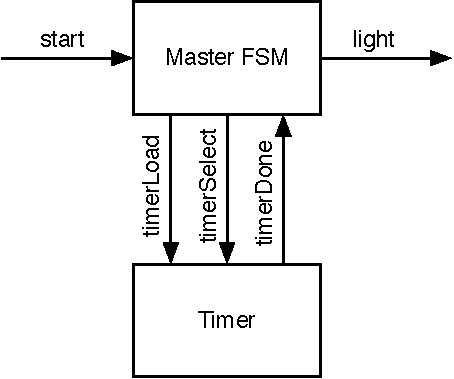
\includegraphics[scale=\scale]{figures/flasher}
  \caption{Mạch chớp đèn tách thành Master FSM và Timer FSM.}
  \label{fig:flasher}
\end{figure}

FSM định thời đếm xuống trong 6 hoặc 4 chu kỳ xung clock để tạo ra thời gian mong muốn. Đặc tả kỹ thuật bộ định thời như sau: 

\begin{itemize}
\item khi \code{timerLoad} được xác nhận, bộ định thời nạp giá trị vào mạch đếm xuống;
\item \code{timerSelect} chọn giữa 5 hoặc 3 để nạp;
\item \code{timerDone} được xác nhận khi mạch đếm hoàn thành đếm xuống và vẫn duy trì xác nhận;
\item nếu không, bộ định thời đếm xuống.
\end{itemize}

\noindent Đoạn mã sau trình bày FSM định thời của mạch chớp đèn:

\shortlist{code/flasher_timer.txt}

\noindent Listing~\ref{lst:flasher:master} trình bày Master FSM.

\longlist{code/flasher_fsm.txt}{Master FSM mạch chớp đèn.}{lst:flasher:master}

\begin{figure}
  \centering
  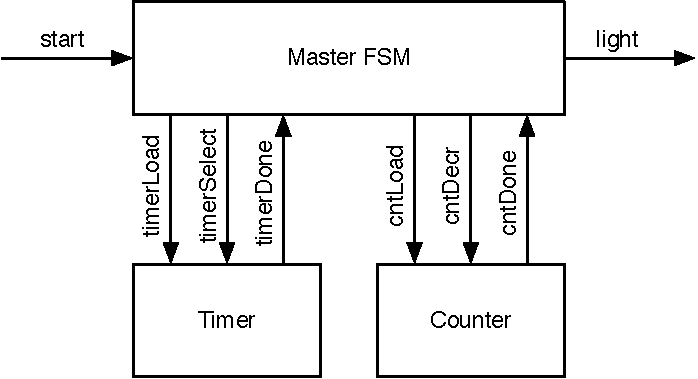
\includegraphics[scale=\scale]{figures/flasher2}
  \caption{Mạch chớp đèn tách thành Master FSM, Timer FSM, và Counter FSM.}
  \label{fig:flasher2}
\end{figure}

Giải pháp này với FSM chủ và một bộ định thời vẫn có sự dư thừa trong mã của FSM chủ. Các trạng thái \code{flash1}, \code{flash2} và \code{flash3} đều đang thực hiện cùng một chức năng, các trạng thái \code{space1} và \code{space2} cũng vậy. Chúng ta có thể phân số lần chớp nháy còn lại vào mạch đếm thứ hai. Sau đó, FSM chủ được giảm xuống còn ba trạng thái: \code{off}, \code{flash} và \code{space}. 

Hình~\ref{fig:flasher2} biểu diễn thiết kế với Master FSM  và hai FSM để đếm: một FSM đếm chu kỳ xung clock trong khoảng thời gian \emph{on} và \emph{off}; FSM thứ hai để đếm số lần chớp nháy còn lại.

Đoạn mã sau trình bày FSM mạch đếm xuống:

\shortlist{code/flasher2_counter.txt}

\noindent Lưu ý rằng bộ đếm được nạp với giá trị 2 cho 3 lần chớp nháy, vì nó đếm số lần nhấp nháy \emph{còn lại} và được giảm dần trong \emph{không gian} trạng thái khi bộ định thời được thực hiện. Listing~\ref{lst:flasher2:master} hiển thị FSM chủ cho mạch chớp nháy tái cấu trúc kép.

\longlist{code/flasher2_fsm.txt}{Master FSM của mạch chớp đèn tái cấu trúc kép.}{lst:flasher2:master}

Bên cạnh việc FSM chủ được giảm xuống chỉ còn ba trạng thái, giải pháp hiện tại của chúng ta cũng có thể cấu hình tốt hơn. Không cần thay đổi FSM nếu chúng ta muốn thay đổi độ dài của khoảng thời gian \emph{on} hoặc \emph{off} hoặc số lần chớp nháy.

Trong phần này, chúng ta đã tìm hiểu các mạch giao tiếp, đặc biệt là FSM, chỉ trao đổi tín hiệu điều khiển. Tuy nhiên, các mạch còn có thể trao đổi dữ liệu. Để trao đổi dữ liệu phối hợp, chúng ta sử dụng tín hiệu bắt tay. Phần tiếp theo mô tả giao tiếp sẵn-sàng-hợp-lệ để kiểm soát luồng trao đổi dữ liệu một chiều. 

\section{Máy trạng thái với đường dữ liệu}
\index{Máy trạng thái với đường dữ liệu}
\index{FSMD}

Một ví dụ tiêu biểu về máy trạng thái giao tiếp là máy trạng thái kết hợp với một đường dữ liệu. Sự kết hợp này thường được gọi là máy trạng thái hữu hạn với đường dữ liệu (Finite State Machine with Datapath - FSMD). Máy trạng thái kiểm soát đường dữ liệu và đường dữ liệu thực hiện tính toán. Ngõ vào FSM là ngõ vào từ môi trường và ngõ vào từ đường dữ liệu. Dữ liệu từ môi trường được đưa vào đường dữ liệu và ngõ ra dữ liệu đến từ đường dữ liệu. Hình~\ref{fig:popcnt-fsmd} biểu diễn một ví dụ về sự kết hợp của FSM với đường dữ liệu. 

\begin{figure}
  \centering
  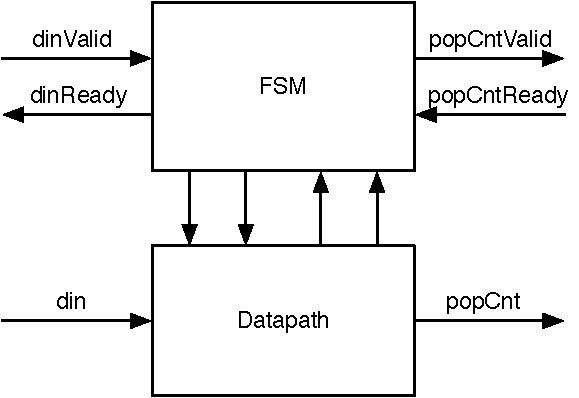
\includegraphics[scale=\scale]{figures/popcnt-fsmd}
  \caption{Máy trạng thái với đường dữ liệu.}
  \label{fig:popcnt-fsmd}
\end{figure}

\subsection{Ví dụ về Popcount}

FSMD được biểu diễn trong Hình~\ref{fig:popcnt-fsmd} đóng vai trò là một ví dụ tính toán Popcount, còn được gọi là \myref{https://en.wikipedia.org/wiki/Hamming_weight}{trọng số Hamming}. Trọng số Hamming là số các ký hiệu khác với ký hiệu số 0. Đối với một chuỗi nhị phân, đây là số lần của số `1'. 

Đơn vị Popcount chứa ngõ vào dữ liệu \code{din} và ngõ ra kết quả \code{popCount}, cả hai đều được kết nối với đường dữ liệu. Đối với ngõ vào và ngõ ra, chúng ta sử dụng một tín hiệu bắt tay sẵn-sàng-hợp-lệ. Khi dữ liệu có sẵn, xác nhận hợp lệ. Khi bộ thu có thể chấp nhận dữ liệu, nó xác nhận rằng nó đã sẵn sàng. Khi cả hai tín hiệu được xác nhận, quá trình chuyển dữ liệu sẽ diễn ra. Các tín hiệu bắt tay được kết nối với FSM. FSM được kết nối với đường dữ liệu với các tín hiệu điều khiển hướng tới đường dữ liệu và với các tín hiệu trạng thái từ đường dữ liệu. 

\index{Đường dữ liệu}

\begin{figure}
  \centering
  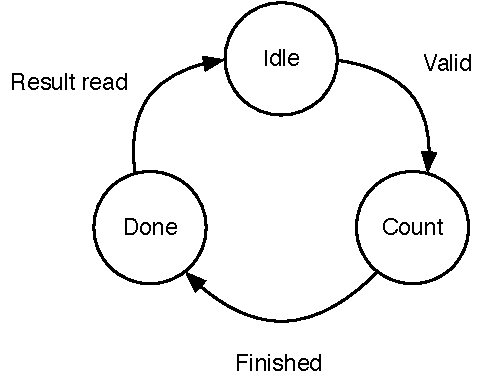
\includegraphics[scale=\scale]{figures/popcnt-states}
  \caption{Lưu đồ trạng thái cho FSM Popcount.}
  \label{fig:popcnt-states}
\end{figure}

Bước tiếp theo, chúng ta có thể thiết kế FSM, bắt đầu với lưu đồ trạng thái, được biểu diễn trong Hình~\ref{fig:popcnt-states}. Chúng ta bắt đầu ở trạng thái \code{Idle}, nơi FSM chờ ở ngõ vào. Khi dữ liệu đến, được báo hiệu bằng tín hiệu hợp lệ, FSM sẽ chuyển sang trạng thái \code{Load} để nạp thanh ghi dịch. FSM chuyển sang trạng thái tiếp theo \code{Count}, số lượng của số `1' được đếm tuần tự. Chúng ta sử dụng một thanh ghi dịch, một mạch cộng, một thanh ghi tích lũy và một mạch đếm xuống để thực hiện tính toán. Khi mạch đếm xuống bằng 0, quá trình hoàn tất và FSM chuyển sang trạng thái \code{Done}. Tại đó FSM báo hiệu bằng một tín hiệu hợp lệ rằng giá trị Popcount đã sẵn sàng được sử dụng. Khi có tín hiệu sẵn sàng từ bộ thu, FSM sẽ chuyển trở lại trạng thái \code{Idle}, sẵn sàng tính toán số lượng Popcount tiếp theo.

Thành phần mức cao nhất (top-level), được hiển thị trong Listing~\ref{lst:pop:top}, khởi tạo FSM và các thành phần của đường dữ liệu và kết nối chúng bởi các kết nối khối. 

\longlist{code/popcnt_main.txt}{Mức top-level của mạch Popcount.
\todo{Bulk connection should be used here (and tested).}}{lst:pop:top}

\begin{figure}
  \centering
  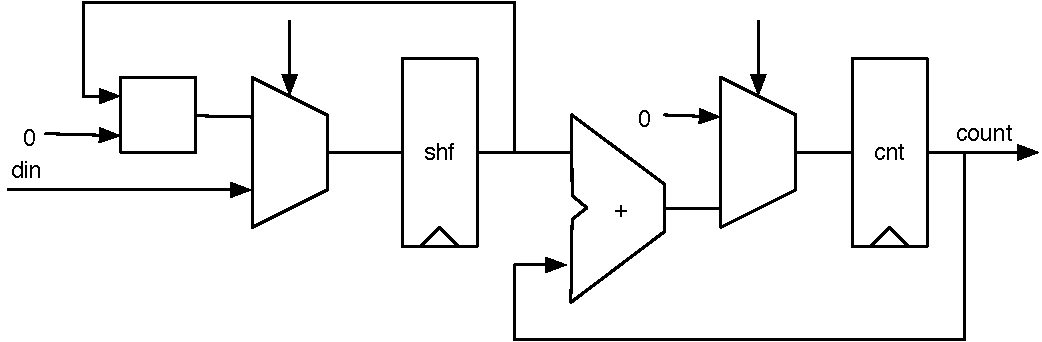
\includegraphics[scale=\scale]{figures/popcnt-data}
  \caption{Đường dữ liệu mạch Popcount.}
  \label{fig:popcnt-data}
\end{figure}

Hình ~\ref{fig:popcnt-data} biểu diễn đường dẫn dữ liệu cho mạch Popcount. Dữ liệu được nạp vào thanh ghi \code{shf}. Khi nạp, thanh ghi \code{cnt} cũng được reset về 0. Để đếm số lượng số `1', thanh ghi \code{shf} được dịch sang phải và bit LSB được thêm vào \code{cnt} mỗi xung clock. Mạch đếm, không được hiển thị trong hình, đếm xuống cho đến khi tất cả các bit được dịch chuyển qua bit LSB. Khi mạch đếm về 0, số lượng Popcount đã hoàn tất. FSM chuyển sang trạng thái \code{Done} và báo hiệu kết quả bằng tín hiệu xác nhận \code{popCntReady}. Khi kết quả được đọc, nó được báo hiệu bằng tín hiệu xác nhận \code{popCntValid}, FSM sẽ chuyển về trạng thái \code{Idle}.

Trên tín hiệu \code{load}, thanh ghi \code{regData} được nạp với giá trị ngõ vào, thanh ghi \code{regPopCount} được reset về 0 và giá trị thanh ghi mạch đếm \code{regCount} được đặt thành số lần dịch đã được thực hiện. 

\longlist{code/popcnt_data.txt}{Đường dữ liệu của mạch Popcount.}{lst:pop:data}
\longlist{code/popcnt_fsm.txt}{FSM của mạch Popcount.}{lst:pop:fsm}

Mặt khác, thanh ghi \code{regData} được dịch sang phải, bit LSB của thanh ghi \code{regData} sẽ được thêm vào thanh ghi \code{regPopCount} và mạch đếm giảm dần cho đến khi nó bằng 0. Khi mạch đếm bằng 0, ngõ ra chứa giá trị Popcount. Listing~\ref{lst:pop:data} trình bày mã Chisel cho đường dữ liệu của mạch Popcount.

FSM bắt đầu ở trạng thái \code{idle}. Với tín hiệu hợp lệ cho dữ liệu ngõ vào (\code{dinValid}), nó sẽ chuyển sang trạng thái \code{count} và đợi đến khi đường dữ liệu hoàn tất việc đếm. Khi Popcount hợp lệ, FSM sẽ chuyển sang trạng thái \code{done} và đợi đến khi giá trị Popcount được đọc (được báo hiệu bằng tín hiệu \code{popCntReady}). Listing~\ref{lst:pop:fsm} trình bày mã code của FSM. 

\section{Giao tiếp sẵn-sàng-hợp-lệ}
\index{Giao tiếp sẵn-sàng-hợp-lệ}

Giao tiếp của các hệ thống con có thể được khái quát hóa thành chuyển động của dữ liệu và bắt tay để điều khiển luồng. Trong ví dụ về Popcount, chúng ta đã thấy một giao diện bắt tay cho dữ liệu ngõ vào và ngõ ra sử dụng các tín hiệu sẵn sàng và hợp lệ. 

\begin{figure}
  \centering
  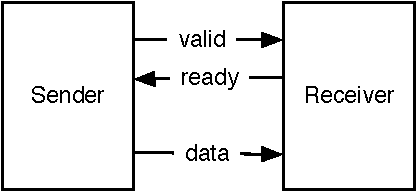
\includegraphics[scale=\scale]{figures/readyvalid}
  \caption{Điều khiển luồng sẵn-sàng-hợp-lệ.}
  \label{fig:readyvalid}
\end{figure}

Giao tiếp sẵn-sàng-hợp-lệ~\cite[p.~480]{dally:vhdl:2016} là một giao tiếp điều khiển luồng đơn giản bao gồm tín hiệu \code{data} và \code{valid} ở phía người gửi (nhà sản xuất) và tín hiệu \code{ready} ở phía người nhận (người tiêu dùng). Hình~\ref{fig:readyvalid} cho thấy kết nối sẵn-sàng-hợp-lệ. Người gửi xác nhận tín hiệu \code{valid} khi \code{data} khả dụng và người nhận xác nhận tín hiệu \code{ready} khi sẵn sàng nhận một word dữ liệu. Việc truyền dữ liệu xảy ra khi cả hai tín hiệu, \code{valid} và \code{ready}, được xác nhận. Nếu một trong hai tín hiệu không được xác nhận, sẽ không có quá trình chuyển dữ liệu nào diễn ra. 

\begin{figure}
  \centering
  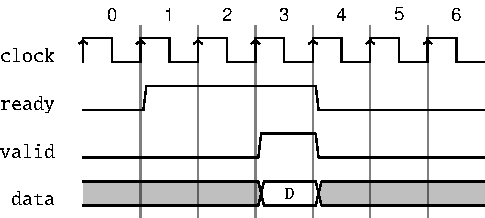
\includegraphics[scale=1]{figures/ready_valid1}
  \caption{Truyền dữ liệu với giao tiếp sẵn-sàng-hợp-lệ, sẵn sàng sớm.}
  \label{fig:ready_valid1}
\end{figure}

Hình~\ref{fig:ready_valid1} biểu diễn sơ đồ thời gian của giao dịch sẵn-sàng-hợp-lệ trong đó bên nhận báo hiệu \code{ready} (từ chu kỳ xung clock 1 trở đi) trước khi bên gửi có dữ liệu. Việc truyền dữ liệu xảy ra trong chu kỳ xung clock 3. Từ chu kỳ xung clock 4 trở đi, cả bên gửi không có dữ liệu và bên nhận không sẵn sàng cho lần truyền tiếp theo. Khi bên nhận có thể nhận dữ liệu trong mọi chu kỳ xung clock, nó được gọi là giao diện ``luôn sẵn sàng'' và tín hiệu \code {ready} có thể được lập trình cố định thành \code{true}. 

\begin{figure}
  \centering
  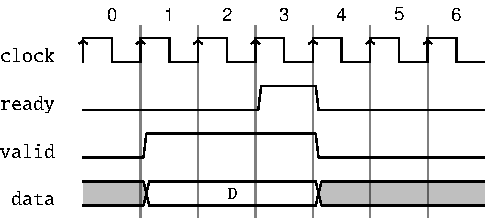
\includegraphics[scale=1]{figures/ready_valid2}
  \caption{Truyền dữ liệu với giao tiếp sẵn-sàng-hợp-lệ, sẵn sàng trễ.}
  \label{fig:ready_valid2}
\end{figure}

Hình~\ref{fig:ready_valid2} biểu diễn sơ đồ thời gian của giao dịch sẵn sàng hợp lệ trong đó bên gửi báo hiệu \code{valid} (từ chu kỳ xung clock 1 trở đi) trước khi bên nhận sẵn sàng. Việc truyền dữ liệu xảy ra trong chu kỳ xung clock 3. Từ chu kỳ xung clock 4 trở đi, cả bên gửi không có dữ liệu và bên nhận không sẵn sàng cho lần truyền tiếp theo. Tương tự như giao tiếp ``luôn sẵn sàng'', chúng ta có thể hình dung và giao tiếp luôn hợp lệ. Tuy nhiên, trong trường hợp đó, dữ liệu có thể sẽ không thay đổi trên tín hiệu \code{ready} và chúng ta sẽ đơn giản bỏ các tín hiệu bắt tay. 

\begin{figure}
  \centering
  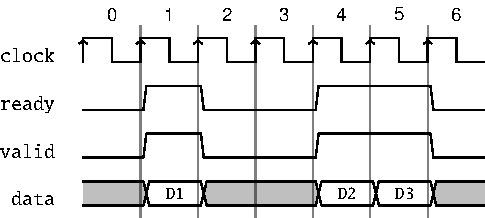
\includegraphics[scale=1]{figures/ready_valid3}
  \caption{Chu kỳ đơn sẵn sàng/hợp lệ và truyền liên tục (back-to-back).}
  \label{fig:ready_valid3}
\end{figure}

Hình~\ref{fig:ready_valid3} biểu diễn các biến thể khác của giao tiếp sẵn-sàng-hợp-lệ. Trong chu kỳ xung clock 1, cả hai tín hiệu (\code{ready} và \code{valid} đều được xác nhận chỉ trong một chu kỳ xung clock duy nhất và quá trình truyền dữ liệu của \code{D1} xảy ra. Dữ liệu có thể được truyền liên tục (trong mọi chu kỳ đồng hồ) như được trình bày trong chu kỳ xung clock 4 và 5 với việc truyền \code{D2} và \code{D3}.

Để làm cho giao tiếp này có thể soạn thảo được, cả tín hiệu \code {ready} và \code{valid} không được phép phụ thuộc vào tổ hợp của tín hiệu khác. Vì giao tiếp này rất phổ biến, nên Chisel định nghĩa \code{DecoupledIO} theo Bundle, tương tự như đoạn mã sau: 

\shortlist{code/fifo_decoupled.txt}

\noindent \code{DecoupledIO} theo Bundle được tham số hóa với kiểu cho \code{data}. Giao tiếp được định nghĩa bởi Chisel sử dụng trường \code{bit} cho dữ liệu.

Vẫn còn một câu hỏi là nếu tín hiệu \code{ready} hoặc \code{valid} có thể bị hủy xác nhận sau khi đang hoạt động và \emph{không} có quá trình truyền dữ liệu nào xảy ra hay không. Ví dụ, một lúc nào đó bên nhận có thể sẵn sàng và không nhận dữ liệu, nhưng do một số sự kiện khác có thể trở nên không sẵn sàng. Điều tương tự có thể được hình dung với bên gửi, dữ liệu chỉ có giá trị hợp lệ trong một số chu kỳ xung clock và trở nên không hợp lệ mà không có truyền dữ liệu. Hành vi này có được phép hay không thì không phải là một phần của giao tiếp sẵn-sàng-hợp-lệ, mà cần được định nghĩa bằng cách sử dụng giao tiếp cụ thể.

Chisel không đặt ra yêu cầu nào về tín hiệu \code{ready} và \code{valid} khi sử dụng lớp \code{DecoupledIO}. Tuy nhiên, lớp \code{IrrevocableIO} đặt ra các hạn chế sau đối với bên gửi:

\begin{quote}
Một lớp con cụ thể của \code{ReadyValidIO} hứa hẹn sẽ không thay đổi giá trị của \code{các bit} sau một chu kỳ, trong đó tín hiệu \code{valid} ở mức cao và tín hiệu \code{ready} ở mức thấp. Ngoài ra, một khi tín hiệu \code{valid} được nâng lên, nó sẽ không bao giờ bị hạ xuống cho đến khi tín hiệu \code{ready} cũng được nâng lên. 
\end{quote}

\noindent Lưu ý rằng, đây là quy ước không thể được thực thi bằng cách sử dụng lớp \code{IrrevocableIO}.

AXI sử dụng một giao tiếp sẵn-sàng-hợp-lệ cho một trong các phần sau của bus: đọc địa chỉ, đọc dữ liệu, ghi địa chỉ và ghi dữ liệu. AXI hạn chế giao tiếp khi tín hiệu \code{ready} hoặc \code{valid} được xác nhận, nó sẽ không được phép hủy xác nhận cho đến khi quá trình truyền dữ liệu diễn ra. 

\todo{Read and cite AXI, and check if the above is true}

\todo{Reconsider writing the testing chapter}

%\chapter{Debugging, Testing, and Verification}
%\index{Debugging}
%\index{Testing}
%\index{Verification}
%
%During your design and coding phase you often debug your design.
%\myref{https://en.wikipedia.org/wiki/Debugging}{Debugging} is the process of
%finding defects in your code. Those defects are called
%\myref{https://en.wikipedia.org/wiki/Software_bug}{bugs}.
%Debugging is often performed in parallel with writing new code.
%
%Testing and verification have slightly different meaning in software development
%and digital design.
%
%\section{Debugging}
%
%One can debug a program by using a debugger or simply by printing interesting
%values to the terminal, called \myref{https://en.wikipedia.org/wiki/Debugging\#printf\_debugging}{printf debugging}.
%In hardware elements are \emph{executing} in parallel. Therefore a common form of hardware
%debugging is generating waveforms and watching how interesting signals evolve over time.
%We call this \emph{waveform debugging}.\footnote{There is no entry in Wikipedia for this,
%we should create one.}
%
%A Chisel tester can generate waveforms, which can be viewed e.g., with \myref{http://gtkwave.sourceforge.net/}{GTKWave}.
%However, for quick checks it is also possible to print signal values during simulation of the circuit.
%Values are printed at the rising edge of the clock.
%
%
%\section{Testing in Chisel}
%
%
%\subsection{Verilator}


\chapter{Bộ tạo phần cứng}
\index{Bộ tạo phần cứng}

Điểm mạnh của Chisel là nó cho phép chúng ta viết cái gọi là bộ tạo phần cứng. Với các ngôn ngữ mô tả phần cứng cũ hơn, chẳng hạn như VHDL và Verilog, chúng ta thường sử dụng một ngôn ngữ khác, ví dụ: Java hoặc Python, để tạo phần cứng. Tác giả thường viết các chương trình Java nhỏ để tạo các bảng VHDL. Trong Chisel, toàn bộ sức mạnh của Scala (và các thư viện Java) là có sẵn khi xây dựng phần cứng. Vì vậy, chúng ta có thể viết các bộ tạo phần cứng của mình ở cùng một ngôn ngữ và thực thi chúng như một phần của quá trình tạo mạch Chisel. 

\section{Một chút tản mạn về Scala}
\index{Scala}

Mục này giới thiệu rất ngắn gọn về Scala. Nó sẽ đủ để viết bộ tạo phần cứng cho Chisel. Để có phần giới thiệu chuyên sâu về Scala, tôi giới thiệu sách của Odersky và cộng sự~\cite{Scala}.

Scala có hai loại biến: \code{val} và \code{var}. Biến \code{val} cung cấp tên cho một biểu thức và không thể gán lại giá trị. Đoạn mã sau đây trình bày định nghĩa của một giá trị số nguyên được gọi là \code{zero}. Nếu chúng ta cố gắng gán lại một giá trị về \code{zero}, chúng ta sẽ gặp lỗi biên dịch. 

\shortlist{code/scala_val.txt}

\noindent Trong Chisel, chúng ta chỉ sử dụng \code{val} để đặt tên các thành phần phần cứng. Lưu ý rằng toán tử \code{:=} là toán tử Chisel và không phải là toán tử Scala.

Scala cũng cung cấp phiên bản cổ điển hơn của một biến như \code{var}. Đoạn mã sau định nghĩa một biến số nguyên và gán lại cho nó một giá trị mới: 

\shortlist{code/scala_var.txt}

\noindent Chúng ta sẽ cần \code{var} trong Scala để viết \emph{các bộ tạo} phần cứng, nhưng không bao giờ cần dùng nó để đặt tên cho một \emph{thành phần} phần cứng.

Các bạn có thể đã tự hỏi xem các biến đó có kiểu gì. Như chúng ta đã gán một hằng số là số nguyên trong ví dụ trên, kiểu của biến được \emph{suy luận ra}; nó là kiểu Scala \code{Int}. Trong hầu hết các trường hợp, trình biên dịch Scala có thể suy ra kiểu. Tuy nhiên, nếu chúng ta muốn rõ ràng hơn, chúng ta có thể khai báo kiểu như sau: 

\shortlist{code/scala_int_type.txt}

Các vòng lặp cơ bản được viết như sau:

\shortlist{code/scala_loop.txt}

Chúng ta sử dụng một vòng lặp cho bộ tạo mạch. Vòng lặp sau kết nối các bit riêng lẻ của một thanh ghi dịch. 

\shortlist{code/scala_loop_gen.txt}

Các lệnh điều kiện được biểu diễn bởi \code{if} và \code{else}. Lưu ý rằng điều kiện này được đánh giá tại thời gian chạy Scala trong quá trình tạo mạch. Cấu trúc này \emph{không} tạo ra mạch đa hợp.

\shortlist{code/scala_condition.txt}

\section{Cấu hình với các tham số}
\index{Các tham số}

Các thành phần và chức năng của Chisel có thể được cấu hình với các tham số. Các tham số có thể đơn giản như một hằng số nguyên, nhưng cũng có thể là một kiểu phần cứng Chisel. 

\subsection{Các tham số đơn giản}

Cách cơ bản để tham số hóa một mạch là định nghĩa độ rộng bit như một tham số. Các tham số có thể được truyền dưới dạng đối số cho bộ tạo cấu trúc của mô-đun Chisel. Ví dụ sau là một ví dụ về một mô-đun thực hiện một mạch cộng với độ rộng bit có thể được cấu hình. Độ rộng bit \code{n} là một tham số (thuộc kiểu Scala \code{Int}) của thành phần được truyền vào bộ tạo cấu trúc, có thể được sử dụng trong gói IO. 

\shortlist{code/param_adder.txt}

\noindent Các phiên bản được tham số hóa của mạch cộng có thể được tạo như sau:

\shortlist{code/use_param_adder.txt}

\subsection{Các hàm với các tham số kiểu}
\index{Tham số kiểu}

Độ rộng bit như một tham số cấu hình chỉ là điểm khởi đầu cho các bộ tạo phần cứng. Một cấu hình rất linh hoạt là việc sử dụng các kiểu. Tính năng đó cho phép Chisel cung cấp một mạch đa hợp (\code{Mux}) có thể chấp nhận bất kỳ kiểu ghép kênh/đa hợp nào. Để chỉ ra cách sử dụng các kiểu cho việc cấu hình, chúng ta xây dựng một mạch đa hợp chấp nhận các kiểu tùy ý. Hàm sau định nghĩa mạch đa hợp: 

\shortlist{code/param_func.txt}

Chisel cho phép tham số hóa các hàm với các kiểu, trong trường hợp với các kiểu Chisel. Biểu thức trong dấu ngoặc vuông \code{[T <: Data]} định nghĩa tập hợp \code{T}, tham số kiểu là \code{Data} hoặc một lớp con của \code{Data}. \code{Data} là gốc của hệ thống kiểu Chisel.

Hàm đa hợp của chúng ta có ba tham số: điều kiện boolean, một tham số cho đường dẫn đúng và một tham số cho đường dẫn sai. Cả hai tham số đường dẫn đều là kiểu \code{T}, một thông tin được cung cấp khi gọi hàm. Bản thân hàm này là thẳng tiến: chúng ta định nghĩa một dây có giá trị mặc định là \code{fPath} và thay đổi giá trị nếu điều kiện đúng với \code{tPath}. Điều kiện này là một hàm đa hợp cổ điển. Ở cuối hàm, chúng ta trả về phần cứng của mạch đa hợp.

Chúng ta có thể sử dụng hàm đa hợp của mình với các kiểu đơn giản như \code{UInt}: 

\shortlist{code/param_func_simple.txt}

\noindent Kiểu của hai đường dẫn mạch đa hợp cần phải giống nhau. Việc sử dụng sai mạch đa hợp sau đây dẫn đến lỗi thời gian chạy: 

\shortlist{code/param_func_wrong.txt}

\noindent Chúng ta định nghĩa kiểu như \code{Bundle} với hai trường:

\shortlist{code/param_func_type.txt}

\noindent Chúng ta có thể định nghĩa các hằng số \code{Bundle} bằng cách tạo một \code{Wire} đầu tiên và sau đó thiết lập các trường con. Sau đó, chúng ta có thể sử dụng mạch đa hợp đã được tham số hóa với kiểu phức tạp này. 

\shortlist{code/param_func_complex.txt}

Trong thiết kế ban đầu của chúng ta về hàm, chúng ta đã sử dụng \code{WireDefault} để tạo một dây có kiểu \code{T} với giá trị mặc định. Nếu chúng ta cần tạo một dây chỉ thuộc kiểu Chisel mà không sử dụng giá trị mặc định, chúng ta có thể sử dụng \code{fPath.cloneType} để lấy kiểu Chisel. Hàm sau đây biểu diễn cách thay thế để lập trình mạch đa hợp. 

\shortlist{code/param_func_alt.txt}

\subsection{Mô-đun với các tham số kiểu}

Chúng ta cũng có thể tham số hóa các mô-đun với các kiểu Chisel. Giả sử chúng ta muốn thiết kế một mạng trên chip (network-on-chip) để di chuyển dữ liệu giữa các lõi xử lý khác nhau. Tuy nhiên, chúng ta không muốn lập trình cứng định dạng dữ liệu trong giao tiếp bộ định tuyến; chúng ta muốn \emph{tham số hóa} nó. Tương tự như tham số kiểu cho một hàm, chúng ta thêm tham số kiểu \code{T} vào bộ tạo cấu trúc mô-đun. Hơn nữa, chúng ta cần có một tham số cho bộ tạo cấu trúc của kiểu đó. Hơn nữa, trong ví dụ này, chúng ta cũng thực hiện số lượng cổng bộ định tuyến có thể cấu hình. 

\shortlist{code/param_mod.txt}

\noindent Để sử dụng bộ định tuyến, đầu tiên cần định nghĩa kiểu dữ liệu mà chúng ta muốn định tuyến, ví dụ như \code{Bundle} trong Chisel:

\shortlist{code/param_mod_type.txt}

\noindent Chúng ta tạo một bộ định tuyến bằng cách chuyển một thực thể của Bundle do người dùng định nghĩa và số lượng cổng cho bộ tạo kiến trúc của bộ định tuyến: 

\shortlist{code/param_mod_use.txt}

\subsection{Các Bundle được tham số hóa}

Trong ví dụ về bộ định tuyến, chúng ta đã sử dụng hai vectơ trường khác nhau cho ngõ vào của bộ định tuyến: một cho địa chỉ và một cho dữ liệu, được tham số hóa. Một giải pháp thanh thoát hơn là có một \code{Bundle} mà bản thân nó đã được tham số hóa. Chẳng hạn như: 

\shortlist{code/param_bundle_issue.txt}

\code{Bundle} có một tham số kiểu \code{T}, là một kiểu con của kiểu \code{Data} trong Chisel. Trong gói, chúng ta định nghĩa một trường \code{dữ liệu} bằng cách gọi \code{cloneType} trên tham số. Tuy nhiên, khi chúng ta sử dụng một tham số bộ tạo cấu trúc, tham số này sẽ trở thành một trường công khai của lớp. Khi Chisel cần sao chép kiểu của \code{Bundle}, ví dụ: khi nó được sử dụng trong \code{Vec}, trường công khai này sẽ cản trở việc sao chép. Một giải pháp (cách giải quyết) cho vấn đề này là đặt trường tham số ở chế độ riêng tư: 

\shortlist{code/param_bundle.txt}

\noindent Với \code{Bundle} mới đó, chúng ta có thể định nghĩa các cổng bộ định tuyến

\shortlist{code/param_mod2.txt}

\noindent và khởi tạo bộ định tuyến với một \code{Port} và lấy \code{Payload} làm tham số:

\shortlist{code/param_mod_use2.txt}

\section{Tạo mạch logic tổ hợp}
\index{Tạo mạch logic}
\index{Tạo bảng logic}
\label{sec:gen:comb:logic}

Trong Chisel, chúng ta có thể dễ dàng tạo mạch logic bằng cách tạo một bảng logic với \code{Vec} trong Chisel từ \code{Array} trong Scala. Chúng ta có thể có dữ liệu trong một tập tin mà chúng ta có thể đọc trong thời gian tạo phần cứng cho bảng logic. Listing~\ref{lst:file:reader} trình bày cách sử dụng lớp \code {Source} từ thư viện chuẩn Scala để đọc tập tin ``data.txt'', chứa các hằng số nguyên trong biểu diễn dạng văn bản.

Đoạn mã có thể được biểu diễn vài dòng như sau:
\begin{chisel}
  val table = VecInit(array.map(_.U(8.W)))
\end{chisel}

\noindent Một mảng Scala \code{Array} có thể được chuyển đổi hoàn toàn thành một chuỗi (\code{Seq}), hỗ trợ hàm ánh xạ \code{map}. \code{map} gọi một hàm trên mỗi phần tử của chuỗi và trả về một chuỗi giá trị trả về của hàm. Hàm \code{\_.U(8.W)} biểu diễn mỗi giá trị \code{Int} từ mảng Scala dưới dạng \code{\_} và thực hiện chuyển đổi từ giá trị \code{Int} trong Scala thành chuỗi ký tự \code{UInt} trong Chisel, với kích thước 8-bit. Đối tượng \code{VecInit} trong Chisel tạo một \code{Vec} trong Chisel từ một chuỗi \code{Seq} của các kiểu Chisel. 

\index{Đọc tập tin}

\longlist{code/file_reader.txt}{Đọc một tập tin văn bản để tạo bảng logic.}{lst:file:reader}

Chúng ta có thể sử dụng toàn bộ sức mạnh của Scala để tạo ra logic (bảng). Ví dụ: tạo một bảng các hằng số điểm cố định để biểu diễn một hàm lượng giác, tính toán các hằng số cho các mạch lọc số hoặc viết một trình hợp ngữ nhỏ trong Scala để tạo mã cho một bộ vi xử lý được viết bằng Chisel. Tất cả các hàm đó có cùng cơ sở mã code (cùng ngôn ngữ) và có thể được thực thi trong quá trình tạo phần cứng. 

\index{Binary-coded decimal}
\index{BCD}

Một ví dụ cổ điển là chuyển đổi một số nhị phân thành biểu diễn số \myref{https://en.wikipedia.org/wiki/Binary-coded_decimal}{BCD} (binary-coded decimal). BCD được sử dụng để biểu diễn một số ở định dạng thập phân sử dụng 4-bit cho mỗi chữ số thập phân. Ví dụ: số thập phân \code{13} ở dạng nhị phân \code{1101} và số BCD được mã hoá thành 1 (hàng chục) và 3 (hàng đơn vị) ở dạng nhị phân: \code{00010011}. BCD cho phép hiển thị số dưới dạng thập phân, một cách biểu diễn các con số thân thiện với người dùng hơn hệ thập lục phân.

Khi sử dụng ngôn ngữ mô tả phần cứng cổ điển, chẳng hạn như Verilog hoặc VHDL, chúng ta sẽ sử dụng script hoặc ngôn ngữ lập trình khác để tạo một bảng như vậy. Chúng ta có thể viết một chương trình Java tính toán bảng để chuyển đổi số nhị phân sang BCD. Chương trình Java đó in ra mã VHDL có thể được đưa vào trong tập tin Project. Chương trình Java có khoảng 100 dòng mã; hầu hết là các mã tạo chuỗi VHDL. Phần quan trọng của việc chuyển đổi chỉ có hai dòng.

Với Chisel, chúng ta có thể tính bảng này trực tiếp như một phần của việc tạo phần cứng. Listing~\ref{lst:bcd} biểu diễn cách tạo bảng để chuyển đổi số nhị phân sang BCD. 

\longlist{code/bcd_table.txt}{Chuyển đổi hệ nhị phân sang BCD.}{lst:bcd}

\section{Sử dụng kế thừa}
\label{sec:inheritance}

\index{Kế thừa}
\index{Hướng đối tượng}

Chisel là một ngôn ngữ hướng đối tượng. Một thành phần phần cứng, \code{mô-đun} Chisel là một lớp Scala. Do đó, chúng ta có thể sử dụng tính kế thừa để đưa một hành vi chung vào một lớp cha. Chúng ta sẽ khám phá cách sử dụng kế thừa với một ví dụ.

Trong Phần~\ref{sec:counter}, chúng ta đã khám phá các dạng mạch đếm khác nhau, có thể được sử dụng để tạo tick tần suất thấp. Giả sử chúng ta muốn khám phá các phiên bản khác nhau đó, ví dụ: để so sánh yêu cầu tài nguyên của chúng. Chúng ta bắt đầu với một lớp trừu tượng để định nghĩa giao tiếp tick: 

\shortlist{code/ticker.txt}

\noindent Listing~\ref{lst:ticker:up} biểu diễn lần thực hiện đầu tiên của lớp trừu tượng đó với một mạch đếm, đếm lên, cho việc tạo tick. 

\longlist{code/up_ticker.txt}{Tạo tick với mạch đếm.}{lst:ticker:up}

Chúng ta có thể kiểm tra tất cả các phiên bản khác nhau của logic \emph{ticker} bằng một testbench duy nhất. Chúng ta \emph{chỉ} cần định nghĩa testbench để chấp nhận các kiểu con của \code{Ticker}. Listing~\ref{lst:ticker:test} biểu diễn mã Chisel cho trình kiểm tra. \code{TickerTester} có nhiều tham số: (1) tham số kiểu \code{[T <: Ticker]} để chấp nhận một \code{Ticker} hoặc bất kỳ lớp nào kế thừa từ \code{Ticker}, (2) thiết kế đang được kiểm tra, thuộc kiểu \code{T} hoặc kiểu con của chúng và (3) số chu kỳ xung clock mà chúng ta mong đợi cho mỗi tick. Trình kiểm tra chờ sự xuất hiện đầu tiên của tick (thời điểm bắt đầu có thể khác đối với các triển khai khác nhau) và sau đó kiểm tra xem \code{tick} có lặp lại sau mỗi $n$ chu kỳ xung clock không. 

\longlist{code/ticker_tester.txt}{Trình kiểm tra cho các phiên bản khác của ticker.}{lst:ticker:test}

Với thực thi lần đầu tiên, dễ dàng của ticker, chúng ta có thể tự kiểm tra trình kiểm tra, có thể bằng cách gỡ lỗi với lệnh \code{println}. Khi chúng ta tự tin rằng ticker đơn giản và trình kiểm tra là chính xác, chúng ta có thể tiếp tục và khám phá thêm hai phiên bản khác của ticker. Listing~\ref{lst:ticker:down} biểu diễn việc tạo tick với mạch đếm xuống đến 0. Listing~\ref{lst:ticker:nerd} biểu diễn phiên bản Nerd đếm xuống đến -1 nhằm sử dụng ít phần cứng hơn bằng cách tránh dùng mạch so sánh. 

\longlist{code/down_ticker.txt}{Tạo tick với mạch đếm xuống.}{lst:ticker:down}

\longlist{code/nerd_ticker.txt}{Tạo tick bằng cách đếm xuống tới -1.}{lst:ticker:nerd}

Chúng ta có thể kiểm tra tất cả ba phiên bản của ticker bằng cách sử dụng các đặc tả kỹ thuật của ScalaTest, tạo các thực thể của các phiên bản khác nhau của ticker và chuyển chúng đến testbench chung. Listing~\ref{lst:ticker:spec} trình bày các đặc tả kỹ thuật. Chúng ta chỉ chạy các bài kiểm tra ticker với lệnh: 

\begin{chisel}
sbt "testOnly TickerSpec"
\end{chisel}

\longlist{code/ticker_spec.txt}{Đặc tả ScalaTest cho kiểm tra ticker.}{lst:ticker:spec}

\section{Tạo phần cứng với lập trình hàm}
\label{sec:functional}

\index{Lập trình hàm}

Scala hỗ trợ lập trình hàm, Chisel cũng vậy. Chúng ta có thể sử dụng các hàm để biểu diễn phần cứng và kết hợp các thành phần phần cứng đó với lập trình hàm (bằng cách sử dụng cái gọi là ``hàm bậc cao''). Chúng ta hãy bắt đầu với một ví dụ đơn giản, tổng của một véc-tơ: 

\shortlist{code/fun_first.txt}

\noindent Đầu tiên, chúng ta định nghĩa phần cứng cho mạch cộng trong hàm \code {add}. Véc-tơ (kiểu \code{Vec}) trong Chisel nằm trong \code{vec}. Phương thức Scala \code{reduce()} kết hợp tất cả các phần tử của một tập hợp với một phép toán nhị phân, tạo ra một giá trị duy nhất. Phương thức \code{reduce()} giảm tuần tự bắt đầu từ bên trái. Nó lấy hai phần tử đầu tiên và thực hiện phép toán. Kết quả sau đó được kết hợp với phần tử tiếp theo, cho đến khi còn lại một kết quả duy nhất.

Hàm để kết hợp với các phần tử được cung cấp dưới dạng tham số để \code {rút gọn}, trong trường hợp này là \code{cộng}, sẽ trả về một mạch cộng. Kết quả phần cứng là một chuỗi các mạch cộng tính toán tổng các phần tử của véc-tơ \code{vec}.

Thay vì định nghĩa hàm \code{cộng} (đơn giản), chúng ta có thể đưa ra phép cộng dưới dạng hàm ẩn danh và sử dụng ký tự đại diện Scala ``\code{\_}'' để biểu diễn hai toán hạng. 

\shortlist{code/fun_func_lit.txt}

\noindent Với câu lệnh một dòng duy nhất này, chúng ta đã tạo ra chuỗi các mạch cộng. Đối với hàm tổng, một chuỗi không phải là cấu hình lý tưởng, một cây sẽ có độ trễ tổ hợp ngắn hơn. Nếu chúng ta không tin tưởng vào công cụ tổng hợp để sắp xếp lại chuỗi mạch cộng, thì có thể sử dụng phương thức \code{ReduceTree} của Chisel để tạo một cây các mạch cộng: 

\shortlist{code/fun_reduce_tree.txt}

Trong một ví dụ chi tiết hơn, chúng ta xây dựng một mạch điện để tìm giá trị nhỏ nhất trong \code{vec}. Để biểu diễn mạch điện này, chúng ta sử dụng một hàm ẩn danh, được gọi là \emph{function Lite} trong Scala. Cú pháp cho một ký tự hàm là các tham số trong dấu ngoặc đơn, theo sau bởi \code{=>}, và theo sau là nội dung hàm (function body): 

\begin{chisel}
  (param) => function body
\end{chisel}

\noindent Ký tự hàm cho hàm tối thiểu sử dụng hai tham số \code{x} và \code{y}, và trả về một mạch đa hợp (\code{Mux}) để so sánh hai tham số và trả về giá trị nhỏ hơn. 

\shortlist{code/fun_min.txt}

Chúng ta hãy cùng mở rộng mạch điện này để trả về không chỉ giá trị tối thiểu từ \code{vec}, mà còn là vị trí (chỉ mục) trong \code{vec}. Để trả về hai giá trị, chúng ta định nghĩa \code{Two} kiểu Bundle để giữ giá trị và chỉ mục. Chúng ta khai báo \code{vecTwo} \code {Vec} có thể giữ các bundle này và kết nối chúng trong một vòng lặp với ngõ vào và chỉ mục gốc trong \code{Vec}.

Như trước đây, khi chúng ta sử dụng một ký tự hàm trong phương thức \code{ReduceTree} của \code{vecTwo}, so sánh trường giá trị trong bundle và trả về bundle hoàn chỉnh từ mạch đa hợp. Giá trị \code{res} trỏ đến bundle chứa vị trí và giá trị nhỏ nhất. 

\shortlist{code/fun_min2.txt}

Với là một biến thể cuối cùng, chúng ta sử dụng nhiều đặc trưng Scala hơn để tránh tạo bundle để trả về giá trị và chỉ mục. Scala có quan niệm về \myref{https://en.wikibooks.org/wiki/Scala/Tuples}{bộ (dữ liệu)}, là chuỗi giá trị bất biến của các kiểu khác nhau. Đoạn mã code sau đây cho thấy ứng dụng của một chuỗi các hàm đối với tuần tự nguyên gốc. Các hàm chuỗi là một mẫu điển hình trong lập trình hàm. Mẫu này cũng có thể được xem như một đường ống của các phép toán.

Hàm đầu tiên (\code{zipWithIndex}) chuyển đổi chuỗi tuần tự nguyên gốc thành một chuỗi các bộ dữ liệu, ở đó phần tử thứ hai là giá trị chỉ mục. Nói chung, hàm \code{zip} hợp nhất hai chuỗi (nén chúng) thành một chuỗi duy nhất chứa hai phần tử dưới dạng bộ dữ liệu. Hàm tiếp theo ánh xạ bộ đôi của \code{UInt} trong Chisel và \code{Int} trong Scala thành hai \code{UInt} trong Chisel. Hàm \code{reduce} cung cấp việc tạo ra kết quả tìm kiếm tối thiểu. Chúng ta so sánh phần tử đầu tiên của bộ dữ liệu trong hai mạch đa hợp và trả về một bộ dữ liệu chứa vị trí và giá trị nhỏ nhất dưới dạng các kiểu \code{UInt} trong Chisel. 

\shortlist{code/fun_min3.txt}

Lưu ý rằng toàn bộ biểu thức hàm sử dụng \code{Vector} trong Scala để giữ các kết quả trung gian, nhưng trả về phần cứng (các mạch đa hợp được kết nối) chỉ bao gồm các kiểu Chisel. Vì chúng ta sử dụng \code{Vector} trong Scala ở đây, nên chúng ta không thể sử dụng \code{ReduceTree}, vốn chỉ có sẵn trên \code{Vec} của Chisel. 

\shortlist{code/fun_min4.txt}

\chapter{Thiết kế ví dụ}

Trong phần này, chúng ta khám phá một số thiết kế mạch số kích thước nhỏ, chẳng hạn như bộ đệm FIFO được sử dụng làm khối xây dựng cho thiết kế lớn hơn. Trong ví dụ khác, chúng ta thiết kế một giao tiếp nối tiếp (còn được gọi là UART), bản thân UART này có thể sử dụng bộ đệm FIFO. 

\section{Bộ đệm FIFO}
\label{sec:fifo}

\index{FIFO}
\index{Bộ đệm FIFO}
\index{Bộ đệm First-in, first-out}

Chúng ta có thể tách bên ghi (bên gửi) và bên đọc (bên nhận) bằng một bộ đệm giữa bên ghi và bên đọc. Bộ đệm chung là bộ đệm vào trước, ra trước (\href{https://en.wikipedia.org/wiki/FIFO_%28computing_and_electronics%29}{FIFO}). 
Hình~\ref{fig:fifo} biểu diễn bên ghi, FIFO và bên đọc. Dữ liệu được đặt vào trong FIFO bởi bên ghi trên \code{din} đưa vào FIFO với tín hiệu \code{write} đang hoạt động. Dữ liệu được đọc từ FIFO bởi bên đọc trên \code{dout} với tín hiệu \code{read} đang hoạt động. 

\begin{figure}
  \centering
  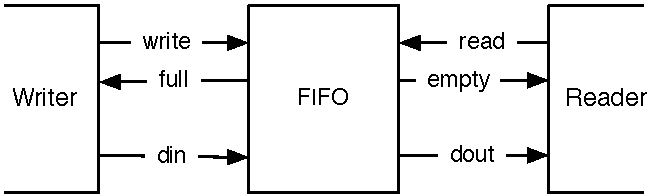
\includegraphics[scale=\scale]{figures/fifo}
  \caption{Bên ghi, bộ đệm FIFO, và bên đọc.}
  \label{fig:fifo}
\end{figure}

Một FIFO ban đầu thường trống được báo hiệu bởi tín hiệu \code{empty}. Việc đọc từ FIFO trống thường không được xác định. Khi dữ liệu được ghi và không bao giờ được đọc, FIFO sẽ trở nên \code{full} (đầy). Việc ghi vào FIFO đầy thường bị bỏ qua và dữ liệu bị mất. Nói cách khác, các tín hiệu \code{empty} và \code{full} đóng vai trò là các tín hiệu bắt tay.

Có thể có nhiều thực hiện khác nhau của FIFO: Ví dụ: sử dụng bộ nhớ trên chip, các con trỏ đọc và ghi, hoặc đơn giản là một chuỗi các thanh ghi với một máy trạng thái nhỏ. Với các bộ đệm nhỏ (khoảng hàng chục phần tử), một FIFO được tổ chức với các thanh ghi riêng lẻ được kết nối thành một chuỗi bộ đệm là một cách thực hiện đơn giản với yêu cầu tài nguyên thấp. Mã code của FIFO bubble có sẵn trong kho lưu trữ \myref{https://github.com/schoeberl/chisel-examples}{chisel-examples}. \footnote{Để hoàn thiện, kho lưu trữ sách Chisel cũng chứa bản sao của mã code FIFO.} 

Chúng ta bắt đầu bằng định nghĩa IO cho bên ghi và bên đọc. Kích thước dữ liệu có thể cấu hình bởi \code{size}. Dữ liệu ghi là \code{din} và một phép ghi được báo hiệu bởi chân \code{write}. Tín hiệu \code{full} thực hiện \myref{https://en.wikipedia.org/wiki/Flow_control_(data)}{điều khiển luồng} ở bên ghi.

\shortlist{code/bubble_fifo_writer_io.txt}

Bên đọc cung cấp dữ liệu với \code{dout} và quá trình đọc được bắt đầu với tín hiệu \code{read}. Tín hiệu \code{empty} chịu trách nhiệm cho việc điều khiển luồng ở bên đọc.

\shortlist{code/bubble_fifo_reader_io.txt}

Listing~\ref{lst:fifo:stage} biểu diễn một bộ đệm đơn. Bộ đệm có cổng xếp hàng \code{enq} của kiểu \code{WriterIO} và cổng rời hàng \code{deq} của kiểu \code{ReaderIO}. Các phần tử trạng thái của bộ đệm là một thanh ghi giữ dữ liệu (\code{dataReg}) và một thanh ghi trạng thái cho FSM đơn giản (\code{stateReg}). FSM chỉ có hai trạng thái: bộ đệm \code{empty} hoặc \code{full}. Nếu bộ đệm \code{empty}, phép ghi sẽ ghi lại dữ liệu ngõ vào và thay đổi thành trạng thái \code{full}. Nếu bộ đệm \code{full}, phép đọc sẽ lấy dữ liệu ra và chuyển sang trạng thái \code{empty}. Các cổng IO \code{full} và \code{empty} biểu diễn trạng thái bộ đệm cho bên ghi và bên đọc. 

\longlist{code/bubble_fifo_register.txt}{Tầng đơn của FIFO bubble.}{lst:fifo:stage}

\index{FIFO bubble}

Listing~\ref{lst:fifo} biểu diễn FIFO hoàn chỉnh. FIFO hoàn chỉnh có giao tiếp IO giống như các bộ đệm FIFO riêng lẻ. \code{BubbleFifo} có các tham số là \code{size} của từ (word) dữ liệu và \code{depth} cho số tầng bộ đệm. Chúng ta có thể xây dựng một FIFO bubble có \code{depth} tầng từ các \code{FifoRegister}. Chúng ta sắp xếp các tầng bằng cách điền chúng vào một kiểu \code{Array} trong Scala. Mảng Scala không có ý nghĩa về phần cứng, nó \emph{chỉ} cung cấp cho chúng ta một vùng chứa để có các tham chiếu đến các bộ đệm đã tạo. Trong vòng lặp \code{for} của Scala, chúng ta kết nối các bộ đệm riêng lẻ. Bên xếp hàng của bộ đệm đầu tiên được kết nối với IO xếp hàng của FIFO hoàn chỉnh và bên rời hàng của bộ đệm cuối cùng nối với bên rời hàng của FIFO hoàn chỉnh. 

\longlist{code/bubble_fifo.txt}{FIFO gồm một mảng các tầng FIFO bubble.}{lst:fifo}

Ý tưởng đã trình bày về việc kết nối các bộ đệm riêng lẻ để thực hiện một hàng đợi FIFO được gọi là FIFO bubble, khi dữ liệu thả nổi (bubble) qua hàng đợi. Điều này đơn giản và là một giải pháp tốt khi tốc độ dữ liệu chậm hơn đáng kể so với tốc độ xung clock, ví dụ, như một bộ đệm tách rời cho cổng nối tiếp sẽ được trình bày trong phần tiếp theo.

Tuy nhiên, khi tốc độ dữ liệu tiếp cận với tần số xung clock, FIFO bubble có hai hạn chế: (1) Vì mỗi trạng thái của bộ đệm phải chuyển đổi giữa \emph{blank} và \emph{full}, có nghĩa là thông lượng tối đa của FIFO là 2 chu kỳ xung clock mỗi từ (word). (2) Dữ liệu cần bubble thông qua FIFO hoàn chỉnh, vì vậy, độ trễ từ ngõ vào đến ngõ ra là số bộ đệm tối thiểu. Tôi sẽ trình bày các thực hiện khả dĩ khác của FIFO trong Phần~\ref{sec:more:fifo}. 

\section{Cổng nối tiếp}
\label{sec:uart}
\index{Cổng nối tiếp}
\index{UART}

Cổng nối tiếp (còn được gọi là \myref{https://en.wikipedia.org/wiki/Universal_asynchronous_receiver-transmitter}{UART} hoặc \myref{https://en.wikipedia.org/wiki/RS-232}{RS-232}) là một trong những tùy chọn dễ dàng nhất để giao tiếp giữa máy tính và bo mạch FPGA. Như tên của nó, dữ liệu được truyền nối tiếp. Một byte 8-bit được truyền như sau: một start bit (0), dữ liệu 8-bit, bit LSB đầu tiên, và sau đó là một hoặc hai stop bit (1). Khi không có dữ liệu nào được truyền, ngõ ra là 1. Hình~\ref{fig:uart:wave} biểu diễn sơ đồ thời gian của một byte được truyền.

\begin{figure}
  \centering
  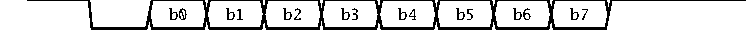
\includegraphics[scale=1]{figures/uart_wave}
  \caption{Một byte được truyền bởi UART.}
  \label{fig:uart:wave}
\end{figure}

Chúng ta thiết kế UART của mình theo cách mô-đun với chức năng tối thiểu trên mỗi mô-đun. Chúng ta trình bày một bộ phát (TX), một bộ thu (RX), một bộ đệm và sau đó là cách sử dụng các thành phần cơ sở đó.

Đầu tiên, chúng ta cần một giao tiếp, một định nghĩa cổng. Đối với thiết kế UART, chúng ta sử dụng giao tiếp bắt tay sẵn sàng/hợp lệ, với hướng (vào/ra) như được thấy từ bộ phát.

\shortlist{code/uart_channel.txt}

Quy ước của giao tiếp sẵn sàng/hợp lệ là dữ liệu được truyền khi cả hai tín hiệu \code{ready} và \code{valid} được xác nhận. 

\longlist{code/uart_tx.txt}{Bộ phát cho cổng nối tiếp.}{lst:uart:tx}

Listing~\ref{lst:uart:tx} biểu diễn một bộ phát nối tiếp cơ bản nhất (\code{Tx}). Các cổng IO là cổng \code{txd}, nơi dữ liệu nối tiếp được gửi và một cổng \code{channel} nơi bộ phát có thể nhận các ký tự để chuyển thành dạng nối tiếp và gửi. Để tạo ra thời gian chính xác, chúng ta tính toán một hằng số bằng cách tính thời gian theo chu kỳ xung clock cho một bit nối tiếp.

Chúng ta sử dụng ba thanh ghi:
(1) thanh ghi để dịch dữ liệu (chuyển dữ liệu thành dạng nối tiếp) (\code{shiftReg}),
(2) một mạch đếm để tạo tốc độ baud chính xác (\code{cntReg}), và
(3) một mạch đếm số bit vẫn cần được dịch ra ngoài.
Không cần thanh ghi trạng thái FSM bổ sung, tất cả trạng thái được mã hóa trong ba thanh ghi đó. 

Mạch đếm \code{cntReg} liên tục chạy (đếm xuống đến 0 và reset về giá trị bắt đầu khi bằng 0). Tất cả hoạt động chỉ được thực hiện khi \code{cntReg} bằng 0. Khi chúng ta xây dựng một bộ phát tối thiểu, chúng ta chỉ có thanh ghi dịch để lưu trữ dữ liệu. Vì vậy, kênh chỉ sẵn sàng khi \code{cntReg} bằng 0 và không còn bit nào để dịch ra ngoài.

Cổng IO \code{txd} được kết nối trực tiếp với bit LSB của thanh ghi dịch. 

Khi có nhiều bit hơn để dịch ra (\code{bitsReg =/= 0.U}), chúng ta dịch các bit sang phải và điền bằng 1 từ mức trên cùng (mức nhàn rỗi của máy phát). Nếu không còn bit nào cần dịch ra ngoài, chúng ta kiểm tra xem kênh có chứa dữ liệu hay không (được báo hiệu bằng cổng \code{valid}). Nếu vậy, chuỗi bit được dịch ra ngoài được xây dựng với một start bit (0), dữ liệu 8-bit và hai stop bit (1). Do đó, số bit đếm được đặt thành 11.

Bộ phát rất tối thiểu này không có bộ đệm bổ sung và chỉ có thể chấp nhận một ký tự mới khi thanh ghi dịch trống và ở chu kỳ xung clock khi \code{cntReg} bằng 0. Chấp nhận dữ liệu mới chỉ khi \code{cntReg} bằng 0 cũng có nghĩa là cờ sẵn sàng cũng được loại bỏ xác nhận khi có chỗ trống trong thanh ghi dịch. Tuy nhiên, chúng tôi không muốn thêm ``độ phức tạp'' này vào bộ phát mà chỉ ủy thác nó vào bộ đệm. 

\longlist{code/uart_buffer.txt}{Bộ đệm byte đơn với giao tiếp sẵn sàng/hợp lệ.}{lst:uart:buffer}

Listing~\ref{lst:uart:buffer} biểu diễn bộ đệm byte đơn, tương tự như thanh ghi FIFO cho FIFO bubble. Cổng ngõ vào là giao tiếp \code{Channel} và ngõ ra là giao tiếp \code{Channel} với các hướng lật. Bộ đệm chứa máy trạng thái tối thiểu để cho biết FIFO là \code{empty} hoặc \code{full}. Các tín hiệu bắt tay điều khiển bộ đệm (\code{in.ready} và \code{out.valid} phụ thuộc vào thanh ghi trạng thái.

Khi trạng thái là \code{empty} và dữ liệu trên ngõ vào là \code{valid}, chúng ta nhận dữ liệu và chuyển sang trạng thái \code{full}. Khi trạng thái là \code{full} và bộ thu phía dưới là \code{ready}, quá trình truyền dữ liệu xuống sẽ xảy ra và chúng chuyển trở lại trạng thái \code{empty}. 

\longlist{code/uart_buffered_tx.txt}{Bộ phát với bộ đệm bổ sung.}{lst:uart:buffered:tx}

Với bộ đệm đó, chúng ta có thể mở rộng bộ phát cơ bản của mình. Listing~\ref{lst:uart:buffered:tx} biểu diễn sự kết hợp của bộ phát \code{Tx} với một bộ đệm đơn phía trước. Bộ đệm này hiện giải quyết vấn đề rằng \code{Tx} chỉ \code {sẵn sàng} cho các chu kỳ xung clock đơn lẻ. Chúng ta đã ủy quyền giải pháp của vấn đề này cho mô-đun bộ đệm. Có thể dễ dàng thực hiện việc mở rộng bộ đệm từ đơn thành FIFO thực và không cần thay đổi bộ phát hoặc bộ đệm byte đơn.

\longlist{code/uart_rx.txt}{Bộ thu cho một cổng nối tiếp.}{lst:uart:rx} 

Listing~\ref{lst:uart:rx} hiển thị mã code cho bộ thu (\code{Rx}). Bộ thu hơi phức tạp một chút vì nó cần phải tái xây dựng lại thời gian của dữ liệu nối tiếp. Bộ thu đợi cho cạnh xuống của start bit. Từ sự kiện đó, bộ thu đợi 1,5 lần bit để định vị chính nó vào giữa bit 0. Sau đó, nó dịch các bit mỗi thời gian của bit. Các bạn có thể quan sát hai lần chờ này với \code {START\_CNT} và \code{BIT\_CNT}. Đối với cả hai lần, cùng một mạch đếm (\code{cntReg}) được sử dụng. Sau khi 8-bit được dịch vào, tín hiệu \code{valReg} báo hiệu một byte có sẵn 

\longlist{code/uart_sender.txt}{Gửi ``Hello World!" qua cổng nối tiếp.}{lst:uart:sender}

Listing~\ref{lst:uart:sender} biểu diễn cách sử dụng bộ phát cổng nối tiếp bằng cách gửi một thông điệp thân thiện ra ngoài. Chúng ta định nghĩa thông điệp trong một chuỗi Scala (\code{msg}) và chuyển đổi nó thành một \code{Vec} trong Chisel của \code{UInt}. Chuỗi Scala là một trình tự hỗ trợ phương pháp \code{ánh xạ}. Phương pháp \code{ánh xạ} nhận đối số là một ký tự của hàm, áp dụng hàm này cho từng phần tử và xây dựng một chuỗi các giá trị trả về của hàm. Nếu ký tự của hàm chỉ có một đối số, như trong trong trường hợp này, đối số có thể được biểu diễn bằng \code{\_}. Ký tự của hàm theo nghĩa đen gọi phương pháp Chisel \code{.U} để chuyển đổi \code{Char} trong Scala thành \code{UInt} trong Chisel. Trình tự sau đó được chuyển tới \code{VecInit} để tạo một \code{Vec} trong Chisel. Chúng ta lập chỉ mục thành véc-tơ \code{văn bản} với mạch đếm \code{cntReg} để cung cấp các ký tự riêng lẻ cho bộ phát được đệm. Với mỗi tín hiệu \code{ready}, chúng ta tăng mạch đếm cho đến khi chuỗi đầy đủ được gửi đi. Bên gửi giữ tín hiệu \code{valid} được xác nhận cho đến khi ký tự cuối cùng được gửi đi. 

\longlist{code/uart_echo.txt}{Dữ liệu dội lại trên cổng nối tiếp.}{lst:uart:echo}

Listing~\ref{lst:uart:echo} biểu diễn cách sử dụng của bộ thu và bộ phát bằng cách kết nối chúng với nhau. Kết nối này tạo ra một mạch \code{Echo} trong đó mỗi ký tự nhận được sẽ được gửi lại (bị dội lại). 

\section{Các biến thể thiết kế FIFO}
\label{sec:more:fifo}

Trong phần này, chúng ta sẽ thực hiện các biến thể khác nhau của hàng đợi FIFO. Để làm cho các thực hiện này có thể hoán đổi cho nhau, chúng ta sẽ sử dụng tính năng thừa kế, như đã giới thiệu trong Phần~\ref{sec:inheritance} 

\subsection{Tham số hóa các FIFO}

Chúng ta định nghĩa một lớp FIFO \code{abstract} với kiểu Chisel làm tham số để có thể đệm bất kỳ kiểu dữ liệu Chisel nào. Trong lớp trừu tượng, chúng ta cũng kiểm tra xem tham số \code{depth} có giá trị hữu ích hay không. 

\shortlist{code/fifo_abstract.txt}

Trong Phần~\ref{sec:fifo}, chúng ta đã định nghĩa các kiểu riêng cho giao tiếp với các tên chung cho các tín hiệu, chẳng hạn như \code{write}, \code{full}, \code{din}, \code{read}, \code{empty} và \code{dout}. Ngõ vào và ngõ ra của bộ đệm như vậy bao gồm dữ liệu và hai tín hiệu để bắt tay (ví dụ: chúng ta ghi vào FIFO qua tín hiệu \code{write} khi nó không bị đầy, báo hiệu bổi tín hiệu \code{full}.

Tuy nhiên, chúng ta có thể khái quát hóa sự bắt tay này thành giao tiếp được gọi là sẵn-sàng-hợp-lệ. Ví dụ: chúng ta có thể xếp hàng một phần tử (ghi vào FIFO) khi FIFO sẵn sàng với \code{ready}. Chúng ta báo hiệu điều này ở bên bộ ghi với tín hiệu \code{valid}. Vì giao tiếp sẵn-sàng-hợp-lệ này rất phổ biến, nên Chisel đưa ra định nghĩa về giao tiếp này trong \code{DecoupledIO} như sau:\footnote{Đây là một sự đơn giản hóa, vì \codefoot{DecoupledIO} thực sự mở rộng một lớp trừu tượng.} 

\shortlist{code/fifo_decoupled.txt}

\noindent Với giao tiếp \code{DecoupledIO}, chúng ta định nghĩa giao tiếp cho FIFO: tín hiệu \code{FifoIO} với cổng xếp hàng \code{enq} và cổng rời hàng \code{deq} bao gồm các giao tiếp sẵn-sàng-hợp-lệ. Giao tiếp \code{DecoupledIO} được định nghĩa từ quan điểm của bên ghi (bên sản xuất). Vì vậy, cổng xếp hàng của FIFO cần lật các hướng tín hiệu.

\index{DecoupledIO}
\index{Giao tiếp sẵn-sàng-hợp-lệ}

\shortlist{code/fifo_io.txt}

Với lớp cơ sở trừu tượng và một giao tiếp, chúng ta có thể chuyên biệt hóa các thực hiện FIFO khác nhau được tối ưu hóa cho các tham số khác nhau (tốc độ, diện tích, công suất hoặc chỉ là sự đơn giản). 

\subsection{Thiết kế lại FIFO Bubble}

Chúng ta có thể định nghĩa lại FIFO bubble từ Phần~\ref{sec:fifo} bằng cách sử dụng các giao tiếp sẵn-sàng-hợp-lệ tiêu chuẩn và có thể được tham số hóa với kiểu dữ liệu Chisel. 

\longlist{code/fifo_bubble.txt}{FIFO bubble với giao tiếp sẵn-sàng-hợp-lệ.}{lst:fifo:bubble}

Listing~\ref{lst:fifo:bubble} biểu diễn FIFO bubble đã được cấu trúc lại với giao tiếp sẵn-sàng-hợp-lệ. Lưu ý những gì chúng ta đặt thành phần \code{Buffer} bên trong từ \code{BubbleFifo} như là lớp riêng. Lớp trợ giúp này chỉ cần thiết cho thành phần này và do đó chúng ta ẩn nó đi và tránh làm ô nhiễm không gian tên. Lớp đệm cũng đã được đơn giản hóa. Thay vì FSM, chúng ta chỉ sử dụng một bit duy nhất, \code{fullReg}, để ghi nhớ trạng thái của bộ đệm: đầy hoặc trống.

FIFO bubble đơn giản, dễ hiểu và sử dụng tài nguyên tối thiểu. Tuy nhiên, vì mỗi tầng bộ đệm phải chuyển đổi giữa trống và đầy, băng thông tối đa của FIFO này là hai chu kỳ xung clock cho mỗi word.

Người ta có thể cân nhắc xem xét cả hai: bên giao tiếp trong bộ đệm để có thể chấp nhận một từ mới khi nhà sản xuất hợp lệ (\code{valid}) và người tiêu dùng sẵn sàng (\code{ready}). Tuy nhiên, điều này đưa ra một đường dẫn tổ hợp từ bắt tay của người tiêu dùng đến bắt tay của nhà sản xuất, điều này vi phạm ngữ nghĩa của giao tiếp sẵn-sàng-hợp-lệ. 

\subsection{FIFO bộ đệm kép}

\index{FIFO bộ đệm kép}

Một giải pháp là giữ trạng thái \code{ready} ngay cả khi thanh ghi bộ đệm nếu đầy. Để có thể chấp nhận một từ dữ liệu từ nhà sản xuất, khi người tiêu dùng không \code{ready}, chúng ta cần một bộ đệm thứ hai, gọi nó là thanh ghi bubble. Khi bộ đệm đầy, dữ liệu mới được lưu trữ trong thanh ghi bubble và tín hiệu \code{ready} bị hủy xác nhận. Khi người tiêu dùng trở lại \code{ready}, dữ liệu được truyền từ thanh ghi dữ liệu đến người tiêu dùng và từ thanh ghi bubble vào thanh ghi dữ liệu. 

\verylonglist{code/fifo_double_buffer.txt}{FIFO với các thành phần bộ đệm kép.}{lst:fifo:double:buffer}

Listing~\ref{lst:fifo:double:buffer} biểu diễn bộ đệm kép. Mỗi thành phần bộ đệm có thể lưu trữ hai lối vào, chúng ta chỉ cần một nửa thành phần bộ đệm (\code{depth/2}). \code{DoubleBuffer} chứa hai thanh ghi, \code{dataReg} và \code{shadowReg}. Người tiêu dùng luôn được phục vụ từ \code{shadowReg}. Bộ đệm kép có ba trạng thái: \code{empty}, \code{one}, và \code{two}, báo hiệu mức lấp đầy của bộ đệm kép. Bộ đệm \code{ready} để chấp nhận dữ liệu mới khi nó ở trạng thái \code{empty} hoặc \code{one}. Dữ liệu hợp lệ khi nó ở trạng thái \code{one} hoặc \code{two}.

Nếu chúng ta chạy FIFO ở tốc độ tối đa và người tiêu dùng luôn \code{ready} thì trạng thái ổn định của bộ đệm kép là \code{one}. Chỉ khi người tiêu dùng hủy xác nhận \code{ready}, hàng đợi sẽ lấp đầy và bộ đệm nhập trạng thái \code{two}. Tuy nhiên, so với FIFO bubble đơn, việc khởi động lại hàng đợi chỉ mất một nửa số chu kỳ xung clock cho cùng dung lượng bộ đệm. Tương tự, độ trễ của FIFO bubble giảm xuống một nửa. 

\subsection{FIFO với bộ nhớ thanh ghi}

Khi các bạn có nền tảng từ kỹ thuật phần mềm, các bạn có thể tự hỏi rằng chúng ta đã xây dựng hàng đợi phần cứng từ nhiều phần tử bộ đệm nhỏ riêng lẻ, tất cả đều thực thi song song và bắt tay với các phần tử luồng lên (upstream) và luồng xuống (downstream). Đối với các vùng đệm nhỏ, đây có lẽ là cách thực hiện hiệu quả nhất. 

\index{Bộ đệm vòng}
\index{Bộ đệm vòng!con trỏ đọc}
\index{Bộ đệm vòng!con trỏ ghi}

Hàng đợi trong phần mềm thường được sử dụng bởi một mã tuần tự trong một luồng duy nhất. Hoặc như một hàng đợi để tách nhà sản xuất và người tiêu dùng. Trong cài đặt này, hàng đợi FIFO có kích thước cố định thường được thực hiện dưới dạng \myref{https://en.wikipedia.org/wiki/Circular_buffer}{bộ đệm vòng}.
Hai con trỏ trỏ vào vị trí đọc và ghi trong tập bộ nhớ riêng cho hàng đợi. Khi các con trỏ đến cuối bộ nhớ, con trỏ được đặt trở lại điểm bắt đầu của bộ nhớ đó. Sự khác biệt giữa hai con trỏ là số phần tử trong hàng đợi. Khi hai con trỏ trỏ đến cùng một địa chỉ, hàng đợi trống hoặc đầy. Để phân biệt giữa trống và đầy, chúng ta cần một cờ khác. 

Chúng ta cũng có thể thực hiện hàng đợi FIFO dựa trên bộ nhớ trên phần cứng. Đối với các hàng đợi nhỏ, chúng ta có thể sử dụng tập tin thanh ghi (tức là \code{Reg(Vec())}). Listing~\ref{lst:fifo:reg:mem} biểu diễn một hàng đợi FIFO được thực hiện với bộ nhớ và các con trỏ đọc và ghi. 

\verylonglist{code/fifo_reg_mem.txt}{FIFO với bộ nhớ dựa trên thanh ghi.}{lst:fifo:reg:mem}

Vì có hai con trỏ hoạt động giống nhau, giá trị được tăng lên trên một hoạt động và được bao quanh ở cuối bộ đệm, nên chúng ta định nghĩa một hàm \code{counter} thực hiện các mạch đếm gói đó. Với \code{log2Ceil(depth).W}, chúng ta tính toán độ dài bit của mạch đếm. Giá trị tiếp theo được tăng lên 1 hoặc bao quanh 0. Mạch đếm chỉ được tăng lên khi ngõ vào \code{incr} là \code{true.B}.

Hơn nữa, vì chúng ta cũng cần giá trị tiếp theo có thể có (tăng lên hoặc quanh 0), nên chúng ta cũng trả về giá trị này từ hàm \code{counter}. Trong Scala, chúng ta có thể trả về cái gọi là \emph{bộ giá trị}, đơn giản là một vùng chứa để giữ nhiều hơn một giá trị. Cú pháp để tạo một bộ giá trị như vậy chỉ đơn giản là gói các giá trị được phân tách bằng dấu phẩy trong dấu ngoặc đơn: 

\index{Bộ dữ liệu}

\begin{chisel}
  val t = (v1, v2)
\end{chisel}

\noindent Chúng ta có thể giải cấu trúc một bộ như vậy bằng cách sử dụng ký hiệu dấu ngoặc đơn ở phía bên trái của phép gán: 

\begin{chisel}
val (x1, x2) = t
\end{chisel}

Đối với bộ nhớ, chúng ta sử dụng một thanh ghi véc-tơ (\code{Reg(Vec(depth, gen))} của kiểu dữ liệu Chisel \code{gen}. Chúng ta định nghĩa hai tín hiệu để tăng con trỏ đọc và ghi, và tạo ra các con trỏ đọc và ghi bằng hàm \code{counter}. Khi cả hai con trỏ bằng nhau, vùng đệm trống hoặc đầy. Chúng ta định nghĩa hai cờ cho khái niệm trống và đầy.

Khi nhà sản xuất xác nhận \code{valid} và FIFO không đầy, chúng ta:
(1) ghi vào bộ đệm, (2) đảm bảo \code{blankReg} bị hủy xác nhận,
(3) đánh dấu bộ đệm đầy nếu con trỏ ghi bắt kịp với con trỏ đọc trong chu kỳ xung clock tiếp theo (so sánh con trỏ đọc hiện tại với con trỏ ghi tiếp theo) và (4) báo hiệu mạch đếm ghi tăng lên.

Khi người tiêu dùng \code{ready} và FIFO không trống, chúng ta:
(1) đảm bảo rằng \code{fullReg} bị hủy xác nhận, 
(2) đánh dấu bộ đệm trống nếu con trỏ đọc bắt kịp với con trỏ ghi trong chu kỳ xung clock tiếp theo và (3) báo hiệu cho mạch đếm đọc tăng lên. 

Ngõ ra của FIFO là phần tử bộ nhớ tại địa chỉ con trỏ đọc. Các cờ sẵn sàng và hợp lệ chỉ đơn giản là bắt nguồn từ các cờ đầy và trống. 

\subsection{FIFO với bộ nhớ trên chip}

Phiên bản cuối cùng của FIFO sử dụng các tập tin thanh ghi để biểu diễn bộ nhớ, đây là một giải pháp tốt cho một FIFO nhỏ. Với FIFO lớn hơn, tốt hơn là sử dụng bộ nhớ trên chip. Listing~\ref{lst:fifo:mem} biểu diễn một FIFO sử dụng bộ nhớ đồng bộ để lưu trữ. 

\verylonglist{code/fifo_mem.txt}{FIFO với bộ nhớ trên chip.}{lst:fifo:mem}

Việc xử lý con trỏ đọc và ghi giống như FIFO bộ nhớ thanh ghi. Tuy nhiên, một bộ nhớ trên chip đồng bộ đưa ra kết quả của việc đọc trong chu kỳ xung clock tiếp theo, nơi việc đọc tập tin thanh ghi có sẵn trong cùng chu kỳ xung clock.

Do đó, chúng ta cần một số FSM bổ sung và một thanh ghi bubble để xử lý độ trễ này. Chúng ta đọc bộ nhớ ra và cung cấp giá trị của đầu hàng đợi cho cổng ngõ ra. Nếu giá trị đó không được sử dụng, chúng ta cần lưu trữ nó trong thanh ghi bubble \code{shadowReg} trong khi đọc giá trị tiếp theo từ bộ nhớ. Máy trạng thái bao gồm ba trạng thái để biểu diễn: (1) FIFO trống, (2) dữ liệu hợp lệ được đọc ra từ bộ nhớ và (3) đầu hàng đợi trong thanh ghi bubble và dữ liệu hợp lệ (phần tử tiếp theo) từ bộ nhớ.

FIFO dựa trên bộ nhớ có thể giữ một cách hiệu quả lượng dữ liệu lớn hơn trong hàng đợi và có độ trễ giảm nhanh. Trong thiết kế cuối cùng, ngõ ra của FIFO có thể đến trực tiếp từ viêc đọc bộ nhớ. Nếu đường dẫn dữ liệu này nằm trong đường dẫn giới hạn của thiết kế, chúng ta có thể dễ dàng thực hiện kỹ thuật đường ống thiết kế của mình bằng cách kết hợp hai FIFO. Listing~\ref{lst:fifo:comb} biểu diễn một sự kết hợp như vậy. Ở ngõ ra của FIFO dựa trên bộ nhớ, chúng ta thêm một FIFO bộ đệm kép một tầng để tách đường đọc bộ nhớ khỏi ngõ ra. 

\longlist{code/fifo_comb.txt}{Kết hợp bộ nhớ dựa trên FIFO với tầng bộ đệm kép.}{lst:fifo:comb}

\section{Bài tập}

Phần bài tập này dài hơn một chút vì nó bao gồm hai bài tập:
(1) khám phá FIFO bubble và thực hiện một thiết kế FIFO khác;
và (2) khám phá UART và mở rộng nó. 
Mã nguồn cho cả hai bài tập được chứa trong kho lưu trữ 
\myref{https://github.com/schoeberl/chisel-examples}{chisel-examples}.

\subsection{Khám phá FIFO Bubble}

Nguồn FIFO cũng bao gồm một trình kiểm tra kích hoạt hành vi đọc và ghi khác nhau và tạo ra một dạng sóng ở dạng
\myref{https://en.wikipedia.org/wiki/Value_change_dump}{VCD (Value Change Dump)}.
Tập tin VCD có thể được xem bởi một chương trình xem dạng sóng, chẳng hạn như
\myref{http://gtkwave.sourceforge.net/}{GTKWave}.
Khám phá FifoTester trong kho lưu trữ
\myref{https://github.com/schoeberl/chisel-examples/blob/master/src/test/scala/simple/FifoTester.scala}{FifoTester}.
Kho lưu trữ chứa tập tin \code{Makefile} để chạy các ví dụ, với ví dụ FIFO, chỉ cần gõ:
\begin{verbatim}
$ make fifo
\end{verbatim}
Lệnh make này sẽ biên dịch FIFO, chạy kiểm tra và khởi động GTKWave để xem dạng sóng. Khám phá trình kiểm tra và dạng sóng đã được tạo ra.

Trong các chu kỳ đầu tiên, trình kiểm tra viết một từ đơn. Chúng ta có thể quan sát dưới dạng sóng làm thế nào một word được thả nổi (bubble) qua FIFO, do đó có tên là \emph{FIFO bubble}. Việc thả nổi này cũng có nghĩa là độ trễ của một word dữ liệu qua FIFO bằng với độ sâu của FIFO.

Bài kiểm tra tiếp theo lấp dữ liệu vào FIFO đến khi nó đầy. Sau đó là tiến hành đọc đơn. Lưu ý cách các word trống bubble từ phía bên đọc của FIFO sang phía bên ghi. Khi FIFO bubble đầy, nó sẽ lấy độ trễ của độ sâu bộ đệm để đọc làm ảnh hưởng đến phía bên ghi. 

Phần cuối của bài kiểm tra chứa một vòng lặp nhằm nỗ lực ghi và đọc ở tốc độ tối đa. Chúng ta có thể thấy FIFO bubble chạy ở băng thông tối đa, là hai chu kỳ đồng hồ cho mỗi word. Tầng đệm luôn đổi trạng thái giữa trống và đầy cho một lần chuyển một word đơn.

FIFO bubble đơn giản và đối với các bộ đệm nhỏ có yêu cầu tài nguyên thấp. Hạn chế chính của FIFO bubble $n$ tầng là: (1) thông lượng tối đa là một word sau mỗi hai chu kỳ xung clock, (2) một word dữ liệu phải di chuyển $n$ chu kỳ xung clock từ cuối bên ghi đến đầu bên đọc, và (3) FIFO đầy đủ cần $n$ chu kỳ xung clock để khởi động lại. 

Những hạn chế này có thể được giải quyết bằng cách thực hiện FIFO với \myref{https://en.wikipedia.org/wiki/Circular_buffer}{bộ đệm vòng}.
Bộ đệm vòng có thể được thực hiện với một bộ nhớ và các con trỏ đọc và ghi. Thực hiện một FIFO dưới dạng bộ đệm vòng có bốn phần tử, sử dụng cùng một giao tiếp và khám phá các hành vi khác nhau với trình kiểm tra. Với thực hiện ban đầu của việc sử dụng bộ đệm vòng, như một lối tắt, dùng một véc-tơ của các thanh ghi (\code{Reg(Vec(4, UInt(size.W)))}).

\subsection{UART}

Với ví dụ UART, các bạn cần một bo mạch FPGA có cổng nối tiếp và cổng nối tiếp cho máy tính của bạn (thường qua kết nối USB). Kết nối cáp nối tiếp giữa bo mạch FPGA và cổng nối tiếp trên máy tính của các bạn. Chạy chương trình terminal, ví dụ: Hyperterm trên Windows hoặc \code{gtkterm} trên Linux: 

\begin{verbatim}
$ gtkterm &
\end{verbatim}

Cấu hình cổng để sử dụng đúng thiết bị, với UART USB, cổng này thường là \code{/dev/ttyUSB0}. Đặt tốc độ baud là 115200 và không có bit chẵn lẻ (parity) hoặc điều khiển luồng (bắt tay). Với lệnh sau, các bạn có thể tạo mã Verilog cho UART:

\begin{verbatim}
$ make uart
\end{verbatim}

Sau đó, sử dụng công cụ tổng hợp mạch để tổng hợp thiết kế. Kho lưu trữ chứa một dự án Quartus cho bo mạch DE2-115 FPGA. Với Quartus, sử dụng nút Play để tổng hợp thiết kế và sau đó cấu hình FPGA. Sau khi cấu hình, các bạn sẽ thấy một thông báo chúc mừng thành công trong terminal. 

Mở rộng ví dụ về đèn LED nhấp nháy bằng UART, và ghi 0 và 1 vào dòng nối tiếp khi đèn LED tắt và bật. Sử dụng \code{BufferedTx}, như trong ví dụ \code{Sender}.

Với ngõ ra chậm của các ký tự (hai ký tự mỗi giây), các bạn có thể ghi dữ liệu vào thanh ghi truyền UART và có thể bỏ qua bắt tay đọc/hợp lệ. Mở rộng ví dụ bằng cách viết các số lặp lại từ 0-9 nhanh như tốc độ baud cho phép. Trong trường hợp này, các bạn phải mở rộng máy trạng thái của mình để thăm dò trạng thái UART để kiểm tra xem bộ đệm truyền có trống hay không.

Mã code ví dụ chỉ chứa một bộ đệm đơn cho \code{Tx}. Vui lòng thêm FIFO mà các bạn đã thực hiện để thêm bộ đệm cho bộ phát và bộ thu. 

\subsection{Khám phá FIFO}

Viết một FIFO đơn giản với 4 phần tử bộ đệm trong các thanh ghi chuyên dụng. Sử dụng các mạch đếm đọc và ghi 2-bit, có thể chỉ làm tràn. Để đơn giản hóa hơn nữa, hãy xem xét tình huống khi các con trỏ đọc và ghi bằng với FIFO trống. Điều này có nghĩa là các bạn có thể lưu trữ tối đa 3 phần tử. Việc đơn giản hóa này sẽ tránh dùng hàm mạch đếm trong ví dụ ở Listing~\ref{lst:fifo:reg:mem} và xử lý trạng thái trống hoặc đầy với cùng giá trị con trỏ. Chúng ta không cần cờ báo trống hoặc cờ báo đầy, vì điều này có thể được dẫn xuất từ các giá trị con trỏ một mình. Thiết kế này đơn giản hơn bao nhiêu? 

Các thiết kế FIFO khác nhau đã được trình bày có sự cân bằng thiết kế khác nhau liên quan đến các thuộc tính sau: (1) thông lượng tối đa, (2) giảm độ trễ, (3) yêu cầu tài nguyên và (4) tần số xung clock cực đại. Khám phá tất cả các biến thể FIFO ở các kích thước khác nhau bằng cách tổng hợp chúng cho một FPGA; mã nguồn có sẵn tại \myref{https://github.com/schoeberl/chisel-examples}{chisel-examples}.
Đâu là đặc điểm của các FIFO có 4-word, 16-word và 256-word? 

\chapter{Thiết kế bộ xử lý}

\index{Bộ xử lý}
\index{Leros}

Là một trong những chương cuối của cuốn sách này, chúng tôi trình bày một dự án cỡ trung bình: thiết kế, mô phỏng và kiểm tra một bộ vi xử lý. Để quản lý dự án này, chúng ta thiết kế một bộ tích lũy đơn giản. Bộ xử lý có tên là \myref{https://leros-dev.github.io/}{Leros} ~\cite{leros:arcs2019} và có sẵn ở dạng mã nguồn mở tại \url{https://github.com/leros-dev/leros}. Chúng tôi muốn đề cập đây là một ví dụ nâng cao và cần có một số kiến thức về kiến trúc máy tính  để làm theo các ví dụ mã code đã trình bày. 

Leros được thiết kế đơn giản, nhưng vẫn là mục tiêu tốt cho trình biên dịch C. Mô tả của tập lệnh nằm gọn trong một trang, xem Bảng~\ref{tab:leros:isa}. Trong bảng đó \code{A} biểu diễn cho bộ tích lũy, \code{PC} là bộ đếm chương trình, \code{i} là giá trị tức thời (0 đến 255), thanh ghi \code{Rn} (với \code{n} từ 0 đến 255), \code{o} là độ lệch nhánh tương đối so với \code{PC} và thanh ghi địa chỉ \code{AR} để truy cập bộ nhớ. 

\begin{table}
\centering
\begin{tabular}{lll}
\toprule
Mã lệnh & Chức năng & Mô tả\\
\midrule
add & A = A + Rn & Cộng thanh ghi Rn và A \\
addi & A = A + i & Cộng giá trị tức thời i và A \\
sub & A = A - Rn & Trừ thanh ghi Rn với A \\
subi & A = A - i & Trừ giá trị tức thời i với A \\
shr & A = A $>>>$ 1 & Dịch phải (logic) A \\
load & A = Rn & Nạp thanh ghi Rn vào A \\
loadi & A = i & Nạp giá trị tức thời i vào A \\
and & A = A and Rn & AND thanh ghi Rn với A \\
andi & A = A and i & AND giá trị tức thời i với A \\
or & A = A or Rn & OR thanh ghi Rn với A \\
ori & A = A or i & OR giá trị tức thời i với A \\
xor & A = A xor Rn & XOR thanh ghi Rn với A \\
xori & A = A xor i & XOR giá trị tức thời i với A \\
loadhi & A$_{15-8}$ = i & Nạp tức thời vào byte thứ hai \\
loadh2i & A$_{23-16}$ = i  & Nạp tức thời vào byte thứ ba \\
loadh3i & A$_{31-24}$ = i & Nạp tức thời vào byte thứ tư \\
store & Rn = A & Lưu A vào thanh ghi Rn \\
jal & PC = A, Rn = PC + 2 & Nhảy tới A và lưu địa chỉ trả về trong Rn \\
ldaddr & AR = A & Nạp thanh ghi địa chỉ AR với A \\
loadind & A = mem[AR+(i $<<$ 2)] & Nạp một word từ bộ nhớ vào A \\
loadindbu & A = mem[AR+i]$_{7-0}$  &  Nạp một byte không dấu từ bộ nhớ vào A \\
storeind & mem[AR+(i $<<$ 2)] = A & Lưu A vào bộ nhớ \\
storeindb & mem[AR+i]$_{7-0}$ = A & Lưu một byte vào bộ nhớ \\
br & PC = PC + o & Rẽ nhánh \\
brz & if A == 0 PC = PC + o & Rẽ nhánh nếu A bằng zero \\
brnz & if A != 0 PC = PC + o  & Rẽ nhánh nếu A khác zero \\
brp & if A $>=$ 0 PC = PC + o & Rẽ nhánh nếu A là số dương \\
brn & if A $<$ 0 PC = PC + o & Rẽ nhánh nếu A là số âm \\
scall & scall A & Gọi hệ thống (simulation hook) \\
\bottomrule
\end{tabular}
\caption{Tập lệnh của Leros.}
\label{tab:leros:isa}
\end{table}

\section{Bắt đầu với ALU}

\index{ALU}
\index{Bộ xử lý!ALU}

Thành phần trung tâm của một bộ xử lý là \myref{https://en.wikipedia.org/wiki/Arithmetic_logic_unit}{đơn vị logic số học}, hay ghi tắt là ALU (Arithmetic Logic Unit). Vì vậy, chúng ta bắt đầu với việc lập trình cho ALU và testbench. Đầu tiên, chúng ta định nghĩa \code{Enum} để biểu diễn các phép toán khác nhau của ALU:

\shortlist{code/leros_types.txt}

\noindent Một ALU luôn có hai toán hạng ngõ vào (gọi là \code{a} và \code{b}), ngõ vào \code{op} (hoặc opcode) để chọn chức năng (phép toán) và một ngõ ra \code{y}. Listing~\ref{lst:leros-alu} trình bày một ALU.

\todo{draw a nice ALU, see Wikipedia}

Đầu tiên chúng ta định nghĩa tên ngắn hơn cho ba ngõ vào. Câu lệnh \code{switch} định nghĩa logic để tính toán \code{res}. Vì vậy, nó được gán mặc định là 0. Câu lệnh switch liệt kê tất cả các phép toán và gán biểu thức cho phù hợp. Tất cả các hoạt động ánh xạ trực tiếp đến một biểu thức Chisel. Cuối cùng, chúng ta gán kết quả \code{res} cho ngõ ra \code{y} của ALU.

\longlist{code/leros_alu.txt}{ALU của Leros.}{lst:leros-alu}

Để kiểm tra, chúng ta viết hàm ALU ở dạng Scala đơn giản, như trình bày trong Listing~\ref{lst:leros-alu-scala}.

\longlist{code/leros_alu_ref.txt}{Hàm ALU Leros được viết bằng Scala.}{lst:leros-alu-scala}

\noindent Dù bản sao phần cứng này, được viết bằng Chisel bởi một triển khai Scala, không phát hiện ra lỗi trong đặc tả; nhưng ít nhất một số kiểm tra đúng đắn cần thực hiện. Chúng ta sử dụng một số giá trị góc làm véc-tơ kiểm tra (test vector): 

\shortlist{code/leros_alu_testvec.txt}

\noindent Chúng ta kiểm tra tất cả các chức năng với các giá trị ở cả hai ngõ vào:

\shortlist{code/leros_alu_test.txt}

\noindent Việc không thể kiểm tra toàn bộ, đầy đủ đối với các đối số 32-bit là lý do chúng tôi chọn một số trường hợp giá trị góc làm giá trị ngõ vào. Bên cạnh việc kiểm tra các trường hợp góc, việc kiểm tra các ngõ vào ngẫu nhiên cũng rất hữu ích: 

\shortlist{code/leros_alu_rand.txt}

\noindent Các bạn có thể chạy các bài kiểm tra trong dự án Leros với lệnh:

\begin{verbatim}
$ sbt "test:runMain leros.AluTester"
\end{verbatim}

và sẽ tạo ra một thông báo thành công tương tự như sau:

\begin{verbatim}
[info] [0.001] SEED 1544507337402
test Alu Success: 70567 tests passed in 70572 cycles taking
3.845715 seconds
[info] [3.825] RAN 70567 CYCLES PASSED
\end{verbatim}

\section{Giải mã lệnh}

\index{Bộ xử lý!giải mã lệnh}

Từ ALU, chúng ta làm ngược lại và thực hiện bộ giải mã lệnh. Tuy nhiên, đầu tiên, chúng ta định nghĩa mã hóa lệnh trong lớp Scala của riêng nó và gói \emph{chia sẻ}. Chúng ta muốn chia sẻ các hằng số mã hóa giữa việc triển khai phần cứng của Leros, một trình hợp dịch cho Leros và một trình mô phỏng tập lệnh của Leros. 

\shortlist{code/leros_constants.txt}

\todo{Update code when Leros is more complete, as stuff is missing.}

\noindent Đối với thành phần giải mã, chúng ta định nghĩa một \code{Bundle} cho ngõ ra, sau này được đưa một phần vào ALU. 

\shortlist{code/leros_decode_bundle.txt}

\noindent Giải mã lấy ngõ vào là mã lệnh 8-bit và chuyển các tín hiệu đã giải mã dưới dạng ngõ ra. Các tín hiệu điều khiển đó được gán một giá trị mặc định với \code{WireDefault}. 

\shortlist{code/leros_decode_init.txt}

\noindent Bản thân việc giải mã chỉ là dùng cú pháp switch trên một phần của lệnh nhằm biểu diễn mã lệnh (trong Leros, hầu hết các lệnh là 8-bit trên.) 

\shortlist{code/leros_decode.txt}

\section{Lệnh hợp ngữ}

\index{Trình hợp dịch}

Để viết chương trình cho Leros, chúng ta cần một trình hợp dịch. Tuy nhiên, đối với thử nghiệm đầu tiên, chúng ta có thể viết mã cứng một vài lệnh và đặt chúng vào một mảng Scala, mảng mà chúng ta sử dụng để khởi tạo bộ nhớ lệnh. 

\shortlist{code/leros_asm_hard.txt}

\noindent Tuy nhiên, đây là một cách tiếp cận rất kém hiệu quả để kiểm tra một bộ xử lý. Viết một trình hợp dịch với ngôn ngữ biểu diễn như Scala không phải là một dự án lớn. Do đó, chúng ta viết một trình hợp ngữ đơn giản cho Leros, có thể trong khoảng 100 dòng mã. Chúng ta định nghĩa một hàm \code{getProgram} gọi trình hợp dịch. Đối với các điểm đích rẽ nhánh, chúng ta cần một bảng ký hiệu, bảng này chúng ta thu thập trong một \code{Map}. Một trình hợp dịch cổ điển chạy hai lần: (1) thu thập các giá trị cho bảng ký hiệu và (2) ráp chương trình với các ký hiệu được thu thập trong lần chạy đầu tiên. Do đó, chúng ta gọi hàm \code{assemble} hai lần với một tham số để cho biết đó là lần chạy nào. 

\shortlist{code/leros_asm_call.txt}

Hàm \code{assemble} bắt đầu với việc đọc trong tập tin nguồn\footnote{Hàm này không thực sự đọc tập tin nguồn, nhưng đối với cuộc thảo luận này, chúng ta có thể coi nó là hàm đọc.} và định nghĩa hai hàm trợ giúp để phân tích cú pháp hai toán hạng có thể gồm: (1) một hằng số nguyên (cho phép ký hiệu thập phân hoặc thập lục phân) và (2) để đọc số thanh ghi. 

\shortlist{code/leros_asm_start.txt}

Listing~\ref{lst:leros-asm-match} trình bày lõi của trình hợp dịch cho Leros. Biểu thức \code{match}trong Scala bao hàm lõi của hàm hợp ngữ. 

\todo{Some more words on the code.}

\longlist{code/leros_asm_match.txt}{Phần chính của trình hợp dịch cho Leros.}{lst:leros-asm-match}

\section{Bài tập}

Bài tập này thuộc một trong những chương cuối cùng ở dạng rất tự do. Các bạn đã kết thúc chuyến tham quan học hỏi của mình thông qua Chisel và sẵn sàng giải quyết các vấn đề thiết kế mà bạn thấy hứng thú.

Một tùy chọn là đọc lại chương này và đọc cùng với tất cả mã nguồn trong \myref{https://github.com/leros-dev/leros}{kho lưu trữ Leros}, chạy các trường hợp kiểm tra, vọc với mã code bằng cách ngừng nó và thấy rằng các bài kiểm tra không chạy.

Một tùy chọn khác là viết chương trình thực hiện Leros của các bạn. Việc thực hiện trong kho lưu trữ chỉ là một phương án tổ chức đường ống khả dĩ. Các bạn có thể viết một phiên bản mô phỏng Chisel của Leros chỉ với một tầng đường ống duy nhất, hoặc Leros siêu đường ống để có tần suất xung clock cao nhất có thể.

Tùy chọn thứ ba là thiết kế bộ xử lý của các bạn ngay từ đầu. Có thể phần trình diễn về cách xây dựng bộ xử lý Leros và các công cụ cần thiết đã thuyết phục các bạn rằng thiết kế và thực hiện bộ xử lý không phải là trò ảo thuật, mà là kỹ thuật có thể mang lại nhiều sự hứng thú. 

\chapter{Đóng góp cho Chisel}

\index{Chisel!Đóng góp}

Chisel là một dự án mã nguồn mở đang được phát triển và cải tiến liên tục. Do đó, các bạn cũng có thể đóng góp cho dự án. Ở đây chúng tôi mô tả cách thiết lập môi trường để phát triển thư viện Chisel và cách đóng góp cho Chisel. 

\section{Thiết lập môi trường phát triển}

Chisel bao gồm nhiều kho chứa khác nhau; tất cả được lưu trữ tại
\myref{https://github.com/freechipsproject}{dự án chip miễn phí trên GitHub}.

Phân nhánh kho lưu trữ mà các bạn muốn đóng góp vào tài khoản GitHub cá nhân của bạn. Các bạn có thể phân nhánh kho lưu trữ bằng cách nhấn nút \code{Fork} trên giao diện web GitHub. Sau đó, từ phân nhánh đó, hãy sao chép phân nhánh của các bạn trong kho lưu trữ\footnote{Lưu ý rằng đối với một sự thay đổi trong firrtl/Chisel, các bạn cũng cần phải phân nhánh và sao chép firrtl}. Trong ví dụ, chúng ta thay đổi \code{chisel3}, và lệnh sao chép cho phân nhánh cục bộ như sau: 

\begin{verbatim}
$ git clone git@github.com:schoeberl/chisel3.git
\end{verbatim}

Để biên dịch Chisel 3 và xuất bản (publish) dưới dạng thực thi thư viện cục bộ:
\begin{verbatim}
$ cd chisel3
$ sbt compile
$ sbt publishLocal
\end{verbatim}

Chú ý trong khi xuất bản, lệnh cục bộ cho chuỗi phiên bản của thư viện đã xuất bản, chứa chuỗi \code{SNAPSHOT}. Nếu các bạn sử dụng trình kiểm tra và phiên bản đã được xuất bản không tương thích với SNAPSHOT của Chisel, hãy phân nhánh và sao chép kho chứa \myref{https://github.com/freechipsproject/chisel-testers}{chisel-tester} và xuất bản nó cục bộ.

Để kiểm tra những thay đổi của mình trong Chisel, các bạn có thể cũng muốn thiết lập dự án Chisel,
ví dụ: bằng cách phân nhánh/sao chép một \myref{https://github.com/schoeberl/chisel-empty}{dự án Chisel trống},
đổi tên nó, và xóa thư mục \code{.git} khỏi nó.

Thay đổi \code{build.sbt} để tham chiếu đến phiên bản Chisel được xuất bản cục bộ.
Hơn nữa, tại thời điểm viết bài này, người đứng đầu mã nguồn Chisel sử dụng Scala phiên bản 2.12, nhưng Scala 2.12 gặp sự cố với \myref{https://github.com/freechipsproject/chisel-template/issues/35}{các gói ẩn danh}. Do đó, các bạn cần thêm tùy chọn Scala sau: \code{"- Xsource: 2.11"}. \code {build.sbt} sẽ trông tương tự như sau: 

\begin{verbatim}
scalaVersion := "2.12.6"

scalacOptions := Seq("-Xsource:2.11")

resolvers ++= Seq(
  Resolver.sonatypeRepo("snapshots"),
  Resolver.sonatypeRepo("releases")
)

libraryDependencies +=
  "edu.berkeley.cs" %% "chisel3" % "3.2-SNAPSHOT"
libraryDependencies +=
  "edu.berkeley.cs" %% "chisel-iotesters" % "1.3-SNAPSHOT"
\end{verbatim}

Biên dịch ứng dụng kiểm tra Chisel của các bạn và xem xét kỹ nếu nó chọn phiên bản được xuất bản cục bộ của thư viện Chisel hay không (cũng có phiên bản SNAPSHOT được xuất bản, vì vậy, nếu phiên bản Scala khác biệt giữa thư viện Chisel và mã ứng dụng của các bạn, thì nó chọn phiên bản SNAPSHOT từ máy chủ thay vì thư viện đã được xuất bản cục bộ của các bạn.)

Xem thêm \myref{https://github.com/freechipsproject/chisel3}{một số ghi chú tại kho chứa Chisel}.

\section{Kiểm tra}

Khi các bạn thay đổi thư viện Chisel, các bạn nên chạy các bài kiểm tra Chisel.
Trong dự án dựa trên \code{sbt}, nó thường được chạy với lệnh sau:

\begin{verbatim}
$ sbt test
\end{verbatim}

Hơn nữa, nếu các bạn thêm chức năng vào, thì các bạn cũng nên cung cấp các bài kiểm tra cho các đặc điểm mới.

\section{Đóng góp với Pull Request}

Trong dự án Chisel, không có nhà phát triển nào cam kết đóng góp trực tiếp đến kho lưu trữ chính. Đóng góp được tổ chức thông qua 
\myref{https://help.github.com/articles/creating-a-pull-request-from-a-fork/}{pull request} (yêu cầu kéo về)
từ một nhánh trong phiên bản phân nhánh của thư viện.
Để biết thêm thông tin, xem thêm tài liệu trên GitHub tại mục
\myref{https://help.github.com/categories/collaborating-with-issues-and-pull-requests/}{đóng góp với pull requests}.
Nhóm Chisel bắt đầu viết tài liệu 
\myref{https://github.com/freechipsproject/chisel-lang-governance/blob/master/reviewer_guidelines.md}{các nguyên tắc đóng góp}.

\section{Bài tập}

Phát minh một toán tử mới cho kiểu \code{UInt}, triển khai nó trong thư viện Chisel và viết một số mã sử dụng/kiểm tra để khám phá toán tử. Nó không cần phải là một toán tử hữu ích; chỉ cần bất cứ thứ gì sẽ tốt, ví dụ: a ? toán tử chuyển cho phía bên trái nếu nó khác 0, nếu ngược lại là bằng 0 thì cho phía bên phải. Nghe giống như một mạch đa hợp, phải không? Bạn cần thêm bao nhiêu dòng mã?\footnote{Việc triển khai nhanh chóng và dễ hiểu chỉ cần hai dòng mã Scala.}

Đơn giản như vậy nhưng vui lòng không mạo hiểm phân nhánh dự án Chisel và thêm các tiện ích mở rộng nhỏ của các bạn. Các thay đổi và mở rộng sẽ được phối hợp với các nhà phát triển chính. Bài tập này chỉ là một bài tập đơn giản để các bạn bắt đầu.

Nếu các bạn táo bạo hơn, các bạn có thể chọn một trong các \myref{https://github.com/freechipsproject/chisel3/issues}{vấn đề mở} và cố gắng giải quyết nó. Sau đó, đóng góp bằng một pull request tới Chisel. Tuy nhiên, có lẽ trước tiên hãy theo dõi phong cách phát triển trong Chisel bằng cách theo dõi các kho lưu trữ GitHub, xem cách các thay đổi và các pull request được xử lý trong dự án mã nguồn mở Chisel. 


\chapter{Tóm lược}
\label{sec:conclusion}

Cuốn sách này trình bày nhập môn thiết kế mạch số sử dụng ngôn ngữ xây dựng phần cứng Chisel. Chúng ta đã thấy một số mạch số đơn giản đến cỡ trung bình được mô tả trong Chisel. Chisel được nhúng trong Scala và do đó kế thừa tính trừu tượng mạnh mẽ của Scala. Vì cuốn sách này nhằm mục đích giới thiệu, nên chúng tôi đã giới hạn các ví dụ với các cách sử dụng đơn giản của Scala. Bước hợp lý tiếp theo là tìm hiểu một vài điều cơ bản về Scala và áp dụng chúng vào dự án Chisel của bạn.

Tôi rất vui khi nhận được phản hồi về cuốn sách, tôi sẽ cải thiện nó hơn nữa và sẽ xuất bản các ấn bản mới. Bạn có thể liên hệ với tôi tại \url{mailto:masca@dtu.dk} hoặc yêu cầu về vấn đề trên hệ thống kho lưu trữ GitHub. Tôi cũng vui vẻ chấp nhận các yêu cầu kéo về từ kho lưu trữ sách nhằm cải tiến và sửa bất kỳ lỗi nào. 

\section*{Truy cập nguồn tài nguyên}

Cuốn sách này có sẵn ở dạng mã nguồn mở. Kho lưu trữ cũng chứa các trang trình bày về khóa học Chisel và tất cả các ví dụ về Chisel: \url{https://github.com/schoeberl/chisel-book}

Một tập hợp các ví dụ cỡ vừa, hầu hết được tham khảo trong cuốn sách, cũng có sẵn ở dạng mã nguồn mở. Bộ tập hợp ví dụ này cũng chứa các tập tin dạng dự án cho các bo mạch FPGA phổ biến khác nhau: \url{https://github.com/schoeberl/chisel-examples} 

\appendix

\chapter{Các dự án Chisel}

\index{Chisel!Các ví dụ}

Chisel không (chưa) được sử dụng trong nhiều dự án. Do đó, việc dùng mã nguồn mở Chisel để học ngôn ngữ và cách lập trình là rất hiếm. Ở đây, chúng tôi liệt kê một vài dự án mà chúng tôi biết đang sử dụng Chisel và có mã nguồn mở. 

\begin{description}

\item[\myref{https://github.com/chipsalliance/rocket-chip}{Rocket Chip}]
là \myref{https://en.wikipedia.org/wiki/RISC-V}{RISC-V}~\cite{risc-v}
Risc là một bộ tạo phức hợp bộ xử lý bao gồm vi kiến trúc Rocket bộ tạo kết nối TileLink. Ban đầu được phát triển tại UC Berkeley như là dự án Chisel quy mô chip đầu tiên ~\cite{rocket:techrep}, Rocket Chip hiện tại được hỗ trợ thương mại hóa bởi \myref{https://www.sifive.com/}{SiFive}.
%The codebase at SiFive serves as a major test bench for Chisel and new Chisel features
%need to pass the tests at SiFive.

\item[\myref{https://github.com/ucb-bar/riscv-sodor}{Sodor}] là một tập hợp các triển khai RISC-V dành cho mục đích giáo dục. Nó chứa 1, 2, 3 và 5 tầng đường ống (pipeline). Tất cả các bộ xử lý đều sử dụng một bộ nhớ vùng tạm đơn giản được chia sẻ bằng cách nạp lệnh, truy cập dữ liệu và tải chương trình thông qua một cổng gỡ lỗi. Sodor chủ yếu được sử dụng trong mô phỏng. 

\item[\myref{https://github.com/t-crest/patmos}{Patmos}] thực hiện bộ xử lý được tối ưu hóa cho các hệ thống thời gian thực ~\cite{patmos:rts2018}. Kho lưu trữ Patmos bao gồm nhiều kiến trúc giao tiếp đa lõi, chẳng hạn như trình phân xử bộ nhớ có thể dự đoán thời gian ~\cite{t-crest:memnoc}, mạng trên chip ~\cite{s4nocni:arcs2019}, bộ nhớ vùng tạm chia sẻ có quyền sở hữu ~\cite{t-crest:ownspm}. Vào thời điểm viết bài này, Patmos vẫn được mô tả trong Chisel 2. 

\item[\myref{https://github.com/pretis/flexpret}{FlexPRET}] là một triển khai của kiến trúc định thời chính xác ~\cite{Zimmer:EECS-2015-181}. FlexPRET triển khai tập lệnh RISC-V và đã được cập nhật lên Chisel 3.1. 

\item[\myref{https://github.com/schoeberl/lipsi}{Lipsi}] là một bộ xử lý nhỏ dành cho các chức năng tiện ích trên hệ thống trên chip (SoC) ~\cite{lipsi:arcs2018}. Vì cơ sở mã của Lipsi rất nhỏ, nó có thể là điểm khởi đầu dễ dàng cho việc thiết kế bộ xử lý trong Chisel. Lipsi cũng trưng bày về năng suất của Chisel/Scala. Tôi đã mất 14 giờ để mô tả phần cứng trong Chisel và chạy nó trên FPGA, viết trình hợp dịch (assembler) trong Scala, viết trình mô phỏng tập lệnh Lipsi trong Scala để đồng mô phỏng và viết một vài trường hợp thử nghiệm trong trình hợp dịch Lipsi. 

\item[\myref{http://www.opensocfabric.org/}{OpenSoC Fabric}] là một trình tạo NoC mã nguồn mở được viết bằng Chisel ~\cite{OpenSoC:ispass2016}. Mục đích nhằm cung cấp một hệ thống trên chip để khám phá thiết kế quy mô lớn. Bản thân NoC là một thiết kế hiện đại với định tuyến lỗ sâu, tín dụng (credits) để kiểm soát luồng và các kênh ảo. OpenSoC Fabric vẫn đang sử dụng Chisel~2. 

\item[\myref{https://github.com/bu-icsg/xfiles-dana}{DANA}] là một bộ tăng tốc mạng nơ-ron, tích hợp với bộ xử lý RISC-V Rocket dùng giao tiếp Rocket Custom Coprocessor (RoCC) ~\cite{RoCC:2015}. DANA hỗ trợ suy luận và học hỏi. 

\item[\myref{https://github.com/antonblanchard/chiselwatt}{Chiselwatt}] là một triển khai của POWER Open ISA. Nó bao gồm tập lệnh để chạy Micropython.

\end{description}

Nếu các bạn biết một dự án nguồn mở sử dụng Chisel, vui lòng gửi cho tôi một ghi chú để tôi có thể đưa nó vào ấn bản của cuốn sách trong tương lai. 

\chapter{Chisel 2}

\index{Chisel 2}

Cuốn sách này bao gồm phiên bản 3 của Chisel. Hơn nữa, Chisel 3 được khuyên dùng cho các thiết kế mới. Tuy nhiên, vẫn còn mã code của Chisel 2 chưa được chuyển đổi sang Chisel 3. Có sẵn tài liệu về cách chuyển đổi tập tin dự án Chisel 2 thành Chisel 3: 

\begin{itemize}
\item \myref{https://github.com/freechipsproject/chisel3/wiki/Chisel3-vs-Chisel2}{Chisel2 so với Chisel3} và
\item \myref{https://github.com/schoeberl/chisel-examples/blob/master/TowardsChisel3.md}{Hướng tới Chisel 3}
\end{itemize}

Tuy nhiên, các bạn có thể tham gia vào một dự án vẫn sử dụng Chisel 2, ví dụ: bộ xử lý \myref{https://github.com/t-crest/patmos}{Patmos} ~\cite{patmos:rts2018}. Vì vậy, chúng tôi cung cấp ở đây một số thông tin về mã Chisel 2 cho những người đã bắt đầu với Chisel 3. 

Đầu tiên, tất cả tài liệu về Chisel 2 đã bị xóa khỏi các trang web của Chisel. Chúng tôi đã lấy lại các tài liệu PDF đó và đưa chúng lên GitHub tại \url{https://github.com/schoeberl/chisel2-doc}. Các bạn có thể sử dụng hướng dẫn Chisel 2 bằng cách chuyển sang nhánh Chisel 2: 

\begin{chisel}
$ git clone https://github.com/ucb-bar/chisel-tutorial.git
$ cd chisel-tutorial
$ git checkout chisel2
\end{chisel}

Sự khác biệt chính có thể nhìn thấy giữa Chisel 3 và 2 là các định nghĩa về hằng số, các bundle cho IO, dây dẫn, bộ nhớ và có thể là các dạng định nghĩa thanh ghi cũ hơn.

Ở một mức độ nào đó, các cấu trúc Chisel 2 có thể được sử dụng trong dự án Chisel 3 bằng cách sử dụng lớp tương thích dùng dưới dạng gói \code{Chisel} thay vì \code{chisel3}. Tuy nhiên, việc sử dụng lớp tương thích này chỉ nên được sử dụng trong giai đoạn chuyển tiếp. Do đó, chúng tôi không trình bày ở đây.

Ở đây là hai ví dụ về các thành phần cơ bản, giống như đã được trình bày cho Chisel 3. Một mô-đun chứa logic tổ hợp: 

\shortlist{chisel2/src/main/scala/Logic.scala}

Lưu ý rằng \code{Bundle} cho định nghĩa IO \emph{không} được bọc trong lớp \code{IO()}. Hơn nữa, hướng của các cổng IO khác nhau được định nghĩa như là một phần của định nghĩa kiểu, trong ví dụ này là \code{INPUT} và \code{OUTPUT} như là một phần của \code{UInt}. Độ rộng được cho là tham số thứ hai. 

\begin{minipage}{\linewidth}
Ví dụ thanh ghi 8-bit trong Chisel 2:

\shortlist{chisel2/src/main/scala/Register.scala}
\end{minipage}

Ở đây, các bạn thấy định nghĩa thanh ghi tiêu biểu với giá trị reset được đưa vào dưới kiểu \code{UInt} cho tham số có tên \code{init}. Dạng này vẫn đúng trong Chisel 3, nhưng việc sử dụng \code{RegInit} và \code{RegNext} được khuyên dùng cho các thiết kế Chisel 3 mới. Cũng lưu ý ở đây là định nghĩa hằng số của 0 có độ rộng 8 bit là \code{UInt(0, 8)}.

Kiểm tra mã C++ và mã Verilog dựa trên Chisel được tạo ra bằng cách gọi \code{chiselMainTest} và \code{chiselMain}. Cả hai hàm ``main'' đều lấy một mảng \code{String} cho các tham số khác. 

\shortlist{chisel2/src/main/scala/LogicTester.scala}

\shortlist{chisel2/src/main/scala/LogicHardware.scala}

Bộ nhớ với các cổng đọc và ghi thanh ghi tuần tự được định nghĩa trong Chisel 2 là: 

\begin{chisel}
  val mem = Mem(UInt(width = 8), 256, seqRead = true)
  val rdData = mem(Reg(next = rdAddr))
  when(wrEna) {
    mem(wrAddr) := wrData
  }
\end{chisel}

\chapter{Các từ viết tắt}

Các nhà thiết kế phần cứng và kỹ sư máy tính thích sử dụng các từ viết tắt. Tuy nhiên, cần thời gian để làm quen với chúng. Dưới đây là danh sách các thuật ngữ phổ biến liên quan đến thiết kế mạch số và kiến trúc máy tính. 

\begin{description}
\item [ADC] analog-to-digital converter
\item [ALU] arithmetic and logic unit
\item [ASIC] application-specific integrated circuit
\item [CFG] control flow graph
\item [Chisel] constructing hardware in a Scala embedded language
\item [CISC] complex instruction set computer
\item [CPI] clock cycles per instruction
\item [CRC] cyclic redundancy check
\item [DAC] digital-to-analog converter
\item [DFF] D flip-flop, data flip-flop
\item [DMA] direct memory access
\item [DRAM] dynamic random access memory
\item [EMC] electromagnetic compatibility
\item [ESD] electrostatic discharge
\item [FF] flip-flop
\item [FIFO] first-in, first-out
\item [FPGA] field-programmable gate array
% \item [GC] garbage collect(ion/or)
\item [HDL] hardware description language
\item [HLS] high-level synthesis
\item [IC] instruction count
\item [IDE] integrated development environment
\item [ILP] instruction level parallelism
\item [IO] input/output
\item [ISA] instruction set architecture
\item [JDK] Java development kit
\item [JIT] just-Iin-time
\item [JVM] Java virtual machine
\item [LC] logic cell
\item [LRU] least-recently used
\item [MMIO] memory-mapped IO
\item [MUX] multiplexer
\item [OO] object oriented
\item [OOO] out-of order
\item [OS] operating system
\item [RISC] reduced instruction set computer
%\item [RT] Real-Time
%\item [RTOS] Real-Time Operating System
\item [SDRAM] synchronous DRAM
\item [SRAM] static random access memory
\item [TOS] top-of stack
\item [UART] universal asynchronous receiver/transmitter
\item [VHDL] VHSIC hardware description language
\item [VHSIC] very high speed integrated circuit
\item [WCET] Worst-Case Execution Time
\end{description}



\bibliographystyle{plain}
\bibliography{chisel}

\printindex

\end{document}

\chapter{Headings}

\todo{Collect the headings here, but only elevate them to chapter level when some
writing is going on.}

\section{Introduction}

 * Why Chisel, what is cool about it
 * What this book is (and what not)
 * Overview of the following Chapters

\section{Basic Circuits}

 * Combinational expressions (basic gates with logic tables)
 * Combinational base circuits (chapter 8 in Culler)
 * Multiplexer (just the simple one for a start)
 * Registers

1. base functions: +, - , and or, register (with reset, with enable)


\section{Build Process and Testing}

 * A full example (blinking LED again)
 * Packages
 * Source organization (Scala)
 * Object to generate Verilog
 * Testing
 * sbt

\section{Components/Modules}

\section{Building Blocks}

 * building blocks (adder, mux, ALU, counter, memory)
 * maybe split into combinational and sequential

\section{Bundles and Vecs (better title needed)}

\section{Medium Complex Circuits (better title needed)}

3. small designs (better name): UART, FIFO, PWM, VGA, sigma delta

\section{State Machines and Data Path}

 * Covered in stuff for Dally book lecture spring 2019

\section{Memory}

 * Vec based ROM with address register
 * Vec based read/write
 * All other variations
 * Escape code in VHDL and Verilog for unsupported memories

\section{Tips and Tricks (better title needed)}

Stuff that saves a little hardware, but might not worse the less readable code

 * Counter to -1
 * Shared adder and subtractor
 * Mux with one hot encoding of select
 * little tricks: count down, add/sub


\section{Scala for Hardware Developers}

 * Simple Scala (for, if else)
 * functions for hardware generation
 * Classes and constructor
 
 \section{More Complex Testing}
 
  * As we know now sone Scala it is time to use the power of Scala for better testing

\section{Hardware Generation}

 * More advanced stuff
 * Table generation (sinus, assembler)
 
 \section{Leros}
 
  * as a more complex design
  4. full design(s): processor

\section{Chisel 2}

 * Some notes for reading Chisel 2 code
 * Update Lipsi to Chisel 3 to work on the 2 to 3 documentation
 
 \section{Chisel Projects}
 
  * Projects written in Chisel, as paper reference, some words and a URL.

\section{Appendix}

 * Basic digital circuits, e.g., transistor based inverter, half and full adder
 * With lot of links to Wikipedia



\end{document}

\subsection*{Course Abstract}

Chisel is a hardware construction language implemented as a domain specific language in Scala. Therefore, the full power of a modern programming language is available to describe hardware and, more important, hardware generators. Chisel has been developed at UC Berkeley and successfully used for several tape outs of RISC-V. Here at DTU we used Chisel in the T-CREST project and in teaching advanced computer architecture.

In this course I will give an overview of Chisel to describe circuits at the RTL, how to use the Chisel tester functionality to test and simulate digital circuits, present how to synthesize circuits for an FPGA, and present advanced functionality of Chisel for the description of circuit generators. Besides lecturing we will have lab sessions to describe small circuits and evaluate them in an FPGA.

The aim of the course is to get a basic understanding of a modern hardware description language and be able to describe simple circuits in Chisel. This course shall give a basis to explore more advanced concepts of circuit generators written in Chisel/Scala.
